\documentclass{amsart}

\usepackage[T1]{fontenc}
\usepackage{enumerate, amsmath, amsfonts, amssymb, amsthm, mathrsfs, wasysym, graphics, graphicx, xcolor, url, hyperref, hypcap, xargs, multicol, pdflscape, multirow, hvfloat, array, ae, aecompl, pifont, mathtools, a4wide, float, blkarray, overpic}
\usepackage[noabbrev,capitalise]{cleveref}
\usepackage[normalem]{ulem}
\usepackage{marginnote}
\hypersetup{colorlinks=true, citecolor=darkblue, linkcolor=darkblue}
\usepackage[all]{xy}
\usepackage{tikz}
\usepackage{tikz-cd}
\usepackage{tkz-graph}
\usetikzlibrary{trees, decorations, decorations.markings, shapes, arrows, matrix, calc, fit, intersections, patterns, angles}
\graphicspath{{figures/}}
\makeatletter\def\input@path{{figures/}}\makeatother
\usepackage{caption}
\captionsetup{width=\textwidth}


%\tikzlibrary{matrix,quotes,arrows.meta}


%%%%%%%%%%%%%%%%%%%%%%%%%%%%%%%%%%%%%%

% theorems
\newtheorem{theorem}{Theorem}[section]
\newtheorem{corollary}[theorem]{Corollary}
\newtheorem{proposition}[theorem]{Proposition}
\newtheorem{lemma}[theorem]{Lemma}
\newtheorem{conjecture}[theorem]{Conjecture}
\newtheorem*{theorem*}{Theorem}%[section]

\theoremstyle{definition}
\newtheorem{definition}[theorem]{Definition}
\newtheorem{example}[theorem]{Example}
\newtheorem{remark}[theorem]{Remark}
\newtheorem{question}[theorem]{Question}
\newtheorem{notation}[theorem]{Notation}
\newtheorem{assumption}[theorem]{Assumption}
\newtheorem{convention}[theorem]{Convention}

\crefname{equation}{Equation}{Equations}

% math special letters
\newcommand{\R}{\mathbb{R}} % reals
\newcommand{\Q}{\mathbb{Q}} % rationals
\newcommand{\N}{\mathbb{N}} % naturals
\newcommand{\Z}{\mathbb{Z}} % integers
\newcommand{\C}{\mathbb{C}} % complex
\newcommand{\I}{\mathbb{I}} % set of integers
\newcommand{\HH}{\mathbb{H}} % hyperplane
\newcommand{\K}{k} % field
\newcommand{\fA}{\mathfrak{A}} % alternating group
\newcommand{\fS}{\mathfrak{S}} % symmetric group
\newcommand{\cA}{\mathcal{A}} % algebra
\newcommand{\cC}{\mathcal{C}} % collection
\newcommand{\cS}{\mathcal{S}} % ground set
\newcommand{\uR}{\underline{R}} % underline set
\newcommand{\uS}{\underline{S}} % underline set
\newcommand{\uT}{\underline{T}} % underline set
\newcommand{\oS}{\overline{S}} % overline set
\newcommand{\ucS}{\underline{\cS}} % underline ground set
\renewcommand{\b}[1]{{\boldsymbol{#1}}} % bold letters
\newcommand{\h}{\widehat} % hat letters

% math commands
\newcommand{\set}[2]{\left\{ #1 \;\middle|\; #2 \right\}} % set notation
\newcommand{\bigset}[2]{\big\{ #1 \;\big|\; #2 \big\}} % big set notation
\newcommand{\Bigset}[2]{\Big\{ #1 \;\Big|\; #2 \Big\}} % Big set notation
\newcommand{\setangle}[2]{\left\langle #1 \;\middle|\; #2 \right\rangle} % set notation
\newcommand{\ssm}{\smallsetminus} % small set minus
\newcommand{\dotprod}[2]{\left\langle \, #1 \; \middle| \; #2 \, \right\rangle} % dot product
\newcommand{\bigdotprod}[2]{\big\langle \, #1 \; \big| \; #2 \, \big\rangle} % dot product
\newcommand{\symdif}{\,\triangle\,} % symmetric difference
\newcommand{\one}{{1\!\!1}} % the all one vector
\newcommand{\eqdef}{\mbox{\,\raisebox{0.2ex}{\scriptsize\ensuremath{\mathrm:}}\ensuremath{=}\,}} % :=
\newcommand{\defeq}{\mbox{~\ensuremath{=}\raisebox{0.2ex}{\scriptsize\ensuremath{\mathrm:}} }} % =:
\newcommand{\simplex}{\triangle} % simplex
\renewcommand{\implies}{\Rightarrow} % imply sign
\newcommand{\transpose}[1]{{#1}^T} % transpose matrix

% operators
\DeclareMathOperator{\conv}{conv} % convex hull
\DeclareMathOperator{\vect}{vect} % linear span
\DeclareMathOperator{\cone}{cone} % cone hull
\DeclareMathOperator{\inv}{inv} % inversions
\DeclareMathOperator{\ascents}{asc} % ascents
\DeclareMathOperator{\descents}{des} % descents

% others
\newcommand{\ie}{\textit{i.e.}~} % id est
\newcommand{\eg}{\textit{e.g.}~} % exempli gratia
\newcommand{\Eg}{\textit{E.g.}~} % exempli gratia
\newcommand{\apriori}{\textit{a priori}} % a priori
\newcommand{\viceversa}{\textit{vice versa}} % vice versa
\newcommand{\versus}{\textit{vs.}~} % versus
\newcommand{\aka}{\textit{a.k.a.}~} % also known as
\newcommand{\perse}{\textit{per se}} % per se
\newcommand{\ordinal}{\textsuperscript{th}} % th for ordinals
\newcommand{\ordinalst}{\textsuperscript{st}} % st for ordinals
\definecolor{darkblue}{rgb}{0,0,0.7} % darkblue color
\definecolor{green}{RGB}{57,181,74} % green color
\definecolor{violet}{RGB}{147,39,143} % violet color
\newcommand{\red}{\color{red}} % red command
\newcommand{\blue}{\color{blue}} % blue command
\newcommand{\orange}{\color{orange}} % orange command
\newcommand{\green}{\color{green}} % green command
\newcommand{\darkblue}{\color{darkblue}} % darkblue command
\newcommand{\defn}[1]{\textsl{\darkblue #1}} % emphasis of a definition
\newcommand{\para}[1]{\medskip\noindent\uline{\textit{#1.}}} % paragraph
\renewcommand{\topfraction}{1} % possibility to have one page of pictures
\renewcommand{\bottomfraction}{1} % possibility to have one page of pictures
\newcommand{\ex}{_{\textrm{exm}}} % examples
\newcommand{\pa}{_{\textrm{pa}}} % path
\newcommand*\circled[1]{\tikz[baseline=(char.base)]{\node[shape=circle,draw,inner sep=1pt, scale=.7] (char) {#1};}}

% marginal comments
\usepackage{todonotes}
\newcommand{\arnau}[1]{\todo[color=orange!30]{#1 --- A.}}
\newcommand{\yann}[1]{\todo[color=red!30]{#1 --- Y.}}
\newcommand{\vincent}[1]{\todo[color=blue!30]{#1 \\ \hfill --- V.}}
\newcommand{\pg}[1]{\todo[color=green!30]{#1 \\ \hfill --- PG.}}

% geometry
\newcommandx{\Asso}[2][1=n,2={}]{\mathsf{Asso}^{#2}(#1)} % associahedron
\newcommandx{\Zono}[2][1=n,2={}]{\mathsf{Zono}^{#2}(#1)} % zonotope
\newcommand{\Fan}{\mathcal{F}} % fan
\newcommand{\multiplicityVector}{\b{m}} % multiplicity vector
\newcommandx{\ray}[1][1=r]{\b{#1}} % ray
\newcommandx{\rays}[1][1=R]{\b{#1}} % rays
\newcommand{\gvector}[1]{\b{g}(#1)} % g-vector of #1
\newcommand{\gvectorFull}[2]{\b{g}(#1,#2)} % g-vector of #2 wrt #1
\newcommand{\gvectors}[1]{\b{g}(#1)} % g-vectors of #1
\newcommand{\gvectorsFull}[2]{\b{g}(#1,#2)} % g-vectors of #2 wrt #1
\newcommandx{\gvectorFan}[1][1=\quiver]{\mathcal{F}(#1)} % g-vector fan
\newcommand{\cvector}[2]{\mathbf{c}(#2 \in #1)} % c-vector of the cluster variable #2 in the cluster #1
\newcommand{\cvectorFull}[3]{\mathbf{c}(#1,#3 \in #2)} % c-vector of the cluster variable #3 in the cluster #2 with respect to the initial cluster #1
\newcommand{\cvectors}[1]{\mathbf{c}(#1)} % c-vectors of the cluster #1
\newcommand{\cvectorsFull}[2]{\mathbf{c}(#1,#2)} % c-vectors of the cluster #2 with respect to the initial cluster #1

% Type cone
\newcommand{\typeCone}{\mathbb{TC}} % type cone
\newcommand{\compatibilityDegree}[2]{(#1\,\|\,#2)} % compatibility degree
\newcommandx{\coefficient}[3][1={\ray[s]}, 2=\ray, 3=\ray']{\alpha_{#2,#3}(#1)} % coefficient in linear dependence

% Cluster algebras
\newcommand{\Trop}[1]{\mathbb{P}_{#1}} % tropical semifield
\newcommand{\positiveExponents}[1]{\left\{#1\right\}_+} % positive exponents in tropical semifield
\newcommand{\negativeExponents}[1]{\left\{#1\right\}_-} % negative exponents in tropical semifield
\newcommand{\seed}{\Sigma} % a cluster
\newcommand{\cluster}{\mathrm{X}} % a cluster
\newcommandx{\clusters}{\mathcal{X}} % all clusters
\newcommand{\coefficients}{\mathrm{P}} % a coefficients tuple
\newcommandx{\variables}[2][1=\B_\circ, 2 = \coefficients_\circ]{\mathcal{V}(#1,#2)} % all variables
\newcommandx{\clusterAlgebra}[2][1=\B_\circ, 2=\coefficients_\circ]{\mathcal{A}\!\left(#1,#2\right)} % cluster algebra
\newcommandx{\principalClusterAlgebra}[1][1=\B_\circ]{\mathcal{A}_{\mathrm{pr}}\left(#1\right)} % principal coefficients cluster algebra
\newcommandx{\coefficientFreeClusterAlgebra}[1][1=\B_\circ]{\mathcal{A}_{\mathrm{fr}}(#1)} % coefficient free cluster algebra
\newcommandx{\clusterComplex}[1][1=\B_\circ]{\Delta(#1)} % cluster complex
\newcommand{\B}{\mathrm{B}} % b-matrix
\newcommand{\A}[1]{\mathrm{A}({#1})} % b-matrix
\newcommand{\D}{\mathrm{D}} % symmetrizer
\newcommand{\simpleRoot}{\alpha} % simple root
\newcommand{\fundamentalWeight}{\omega} % fundamental weights

% Gentle associahedra
\newcommand{\quiver}{\bar Q} % quiver
\newcommand{\blossom}{^\text{\ding{96}}} % blossom
\newcommandx{\strings}[1][1=\quiver]{\mathcal{S}(#1)} % strings
\newcommandx{\distinguishableStrings}[1][1=\quiver]{\mathcal{S}_\mathrm{dist}(#1)} % distinguishable strings
\newcommandx{\walks}[1][1=\quiver]{\mathcal{W}(#1)} % walks
\newcommandx{\properWalks}[1][1=\quiver]{\mathcal{W}_\mathrm{prop}(#1)} % proper walks
\renewcommand{\top}{\mathrm{top}} % top
\newcommand{\bottom}{\mathrm{bot}} % bottom
\newcommandx{\NKC}[1][1=\quiver]{\mathcal{NK}(#1)} % non-kissing complex
\newcommandx{\RNKC}[1][1=\quiver]{\mathcal{RNK}(#1)} % reduced non-kissing complex
\newcommand{\peaks}[1]{\mathsf{peaks}(#1)} % peaks
\newcommand{\deeps}[1]{\mathsf{deeps}(#1)} % deeps
\newcommand{\KN}{\textsc{kn}} % Kissing Number
\newcommand{\hL}{\text{\rotatebox[origin=c]{180}{\checked}}}
\newcommand{\hR}{\text{\rotatebox[origin=c]{180}{\reflectbox{\checked}}}}
\newcommand{\cL}{\text{\reflectbox{\checked}}}
\newcommand{\cR}{\text{\checked}}
\newcommand{\hh}[1]{\hL#1\hR} % hook - hook
\newcommand{\cc}[1]{\cL#1\cR} % cohook - cohook
\newcommand{\hc}[1]{\hL#1\cR} % hook - cohook
\newcommand{\ch}[1]{\cL#1\hR} % cohook - hook
\newcommand{\distinguishedString}[2]{\mathsf{ds}(#1,#2)} % distinguished string
\newcommand{\distinguishedSign}[2]{\varepsilon(#1,#2)} % distinguished sign

% Graph associahedra
\newcommand{\ground}{V} % ground set
\newcommandx{\graphG}[1][1=G]{#1} % graph
\newcommandx{\tube}[1][1=t]{\mathsf{#1}} % tube
\newcommandx{\tubes}{\mathcal{T}} % all tubes
\newcommandx{\tubing}[1][1=T]{\mathsf{#1}} % tubing
\newcommand{\connectedComponents}{\kappa} % connected components
\newcommand{\nestedComplex}{\mathcal{N}} % nested complex
\newcommand{\nonDisconnecting}{\mathrm{nd}} % non-disconnecting vertices
\newcommand{\neighbors}{\mathrm{ne}} % neighbors

% PG et Yann
\newcommand{\field}{\mathbb{K}}
\newcommand{\cat}{\mathcal{C}}
\newcommand{\Hom}[1]{\operatorname{Hom}_{#1}}
\newcommand{\susp}{\Sigma}
\newcommand{\add}{\operatorname{add}}
\newcommand{\MOD}{\operatorname{mod}}
\newcommand{\End}[1]{\operatorname{End}_{#1}}
\newcommand{\spl}{\operatorname{sp}}
\newcommand{\Ksp}{K_0^{\spl}}
\newcommand{\Kg}{K_0^{\b{g}}}
\newcommand{\ind}{\operatorname{ind}}
\newcommand{\coker}{\operatorname{coker}}
\newcommand{\CC}{\phi}
\newcommand{\proj}{\operatorname{proj}}

% extriangulated
\newcommand{\tc}{\mathcal{T}}
\newcommand{\ec}{\mathcal{E}}
\newcommand{\infl}{\rightarrowtail}
\newcommand{\defl}{\twoheadrightarrow}
\newcommand{\Modt}{\operatorname{Mod}\tc}
\newcommand{\modt}{\MOD\tc}
\newcommand{\kzero}[1]{K_0(#1)}
\newcommand{\eps}{\varepsilon}

%% SPECIFIC NON-KISSING COMPLEX
%
%% COMBINATORICS
%% quiver
%
%% walks
%\newcommand{\peaks}[1]{\mathsf{peaks}(#1)} % peaks
%\newcommand{\deeps}[1]{\mathsf{deeps}(#1)} % deeps
%\newcommand{\distinguishedWalk}[2]{\mathsf{dw}(#1,#2)} % distinguished walk
%\newcommand{\distinguishedArrows}[2]{\mathsf{da}(#1,#2)} % distinguished arrows
%\newcommand{\distinguishedString}[2]{\mathsf{ds}(#1,#2)} % distinguished string
%\newcommand{\distinguishedSign}[2]{\varepsilon(#1,#2)} % distinguished sign
%
%% non-kissing complex, lattice, flip graph
%\newcommand{\kn}{\kappa} % kissing number
%\newcommand{\KN}{\textsc{kn}} % Kissing Number
%\newcommandx{\NKC}[1][1=\quiver]{\mathcal{K}_{\mathrm{nk}}(#1)} % non-kissing complex
%\newcommandx{\RNKC}[1][1=\quiver]{\mathcal{C}_{\mathrm{nk}}(#1)} % non-kissing complex
%\newcommandx{\NKL}[1][1=\quiver]{\mathcal{L}_{\mathrm{nk}}(#1)} % non-kissing lattice
%\newcommandx{\NKG}[1][1=\quiver]{\mathcal{G}_{\mathrm{nk}}(#1)} % non-kissing flip graph
%\newcommandx{\NFC}[1][1=\quiver]{\mathcal{C}_{\mathrm{nf}}(#1)} % non-friendly complex
%\newcommand{\peak}{\mathrm{peak}} % bottom dissection
%\newcommand{\deep}{\mathrm{deep}} % top dissection
%\newcommand{\reversed}[1]{#1^{\mathrm{rev}}} % reverse all arrows
%\renewcommand{\top}{\mathrm{top}} % top
%\newcommand{\bottom}{\mathrm{bot}} % bottom
%\newcommand{\walk}{\operatorname{\omega}} % walk (of a curve)
%
%% accordion and slalom complexes
%\newcommand{\surface}{\mathcal{S}} % an orientable surface
%\newcommand{\dual}{^*} % duality
%\newcommand{\dissection}{\mathrm{D}} % dissection of a marked surface
%\newcommand{\vertices}{\mathcal{V}} % vertices of a dissection
%\newcommand{\edges}{\mathcal{E}} % edges of a dissection
%\newcommand{\faces}{\mathcal{F}} % faces of a dissection
%\renewcommandx{\AC}[1][1=\dissection]{\mathcal{K}_{\mathrm{acc}}(#1)} % accordion complex
%\newcommandx{\RAC}[1][1=\dissection]{\mathcal{C}_{\mathrm{acc}}(#1)} % reduced accordion complex
%\newcommandx{\SC}[1][1=\dissection\dual]{\mathcal{K}_{\mathrm{sla}}(#1)} % slalom complex
%\newcommandx{\RSC}[1][1=\dissection\dual]{\mathcal{C}_{\mathrm{sla}}(#1)} % reduced slalom complex
%\newcommandx{\NCC}[1][1={\dissection, \dissection\dual}]{\mathcal{K}_{\mathrm{nc}}(#1)} % non-crossing complex
%\newcommandx{\RNCC}[1][1={\dissection, \dissection\dual}]{\mathcal{C}_{\mathrm{nc}}(#1)} % non-crossing complex
%\newcommand{\curveof}{\operatorname{\gamma}} % curve (of a walk)
%\newcommand{\edgeof}{\operatorname{\varepsilon}} % arc of a vertex
%\newcommand{\dualedgeof}{\operatorname{\varepsilon}\dual} % dual arc of a vertex
%\DeclareRobustCommand{\SSS}{\reflectbox{$\mathsf{Z}$}} % S
%\DeclareRobustCommand{\ZZZ}{\mathsf{Z}} % Z
%\newcommand{\vnext}[1]{#1_{\operatorname{next}}} % next point on the boundary of the surface
%\newcommand{\vprevious}[1]{#1_{\operatorname{prev}}} % previous point on the boundary of the surface
%
%% lattices
%\newcommand{\meet}{\wedge} % meet
%\newcommand{\join}{\vee} % join
%\newcommand{\bigMeet}{\bigwedge} % meet
%\newcommand{\bigJoin}{\bigvee} % join
%\newcommand{\closure}[1]{#1^{\mathrm{cl}}} % closure operator
%\newcommand{\coclosure}[1]{#1^{\mathrm{cocl}}} % coclosure operator
%\newcommand{\uclosure}[1]{#1^{\underline{\mathrm{cl}}}} % loop free closure operator
%\newcommand{\Bicl}[1]{\mathsf{Bic}(#1)} % biclosed sets
%\newcommand{\projDown}{\pi_\downarrow} % down projection map
%\newcommand{\projUp}{\pi^\uparrow} % up projection map
%\newcommand{\JI}{\mathsf{JI}} % join-irreducible
%\newcommand{\MI}{\mathsf{MI}} % meet-irreducible
%\newcommand{\Cong}{\mathsf{Cong}} % congruence lattice
%\newcommand{\con}{\mathrm{con}} % congruence contracting a cover relation
%\newcommand{\ji}{\mathsf{ji}} % join irreducible
%\newcommand{\mi}{\mathsf{mi}} % meet irreducible
%
%% GEOMETRY
%% d-vectors
%\newcommand{\dvector}[1]{\mathbf{d}(#1)} % d-vector of the path #1
%\newcommand{\dvectors}[1]{\mathbf{d}(#1)} % d-vectors of the paths #1
%\newcommandx{\dvectorFan}[1][1=\quiver]{\mathcal{F}^\mathbf{d}(#1)} % d-vector fan
%% g-vectors
%\newcommand{\gvector}[1]{\mathbf{g}(#1)} % g-vector of the path #1
%\newcommand{\gvectors}[1]{\mathbf{g}(#1)} % g-vectors of the paths #1
%\newcommandx{\gvectorFan}[1][1=\quiver]{\mathcal{F}^\mathbf{g}(#1)} % g-vector fan
%% c-vectors
%\newcommand{\cvector}[2]{\mathbf{c}(#1 \in #2)} % c-vector of the path #1 in the facet #2
%\newcommand{\cvectors}[1]{\mathbf{c}(#1)} % c-vectors of the paths #1
%\newcommandx{\allcvectors}[1][1=\quiver]{\mathbf{C}(#1)} % all c-vectors with respect to the initial cluster #1
%\newcommandx{\cvectorFan}[1][1=\quiver]{\mathcal{F}^\mathbf{c}(#1)} % fan of hyperplanes orthogonal to all c-vectors
%% points, hyperplanes, half-spaces
%\newcommand{\point}[1]{\mathbf{p}(#1)} % vertex of the grid associahedron corresponding to the cluster #1
%\newcommandx{\ray}[1][1=r]{\mathbf{#1}} % ray
%\newcommandx{\rays}[1][1=R]{\mathbf{#1}} % rays
%\newcommand{\hs}{\mathbf{H}^{\le}} % half space
%\newcommand{\HS}[1]{\mathbf{H}^{\le}(#1)} % half space
%\newcommand{\hyp}{\mathbf{H}^{=}} % hyperplane
%\newcommand{\Hyp}[1]{\mathbf{H}^{=}(#1)} % hyperplane
%\newcommand{\fix}[1]{\mathrm{Fix}(#1)} % fix space
%
%% ALGEBRA
%\newcommand{\Hom}[1]{\operatorname{{\rm Hom}}_{#1}}
%\newcommand{\Ext}[1]{\operatorname{{\rm Ext}}_{#1}}
%\newcommandx{\AR}[1][1=\quiver]{\mathrm{AR}(#1)} % Auslander-Reiten quiver
%\newcommandx{\tTC}[1][1=\quiver]{\mathcal{K}^{\textrm{s$\tau$-tilt}}(#1)} % tau-tilting complex
%\newcommand{\rep}{\operatorname{{\rm rep}}}
%\newcommand{\proj}{\operatorname{{\rm proj}}}
%\newcommand{\koszul}{^!} % duality

%% formating the part command
%\makeatletter
%\def\part{\@startsection{part}{1}%
%\z@{.7\linespacing\@plus\linespacing}{.8\linespacing}%
%{\LARGE\sffamily\centering}}
%\@addtoreset{section}{part}
%\makeatother
%\renewcommand{\thesection}{\arabic{part}.\arabic{section}}

% formating the table of contents
\makeatletter
\def\l@section{\@tocline{1}{2pt}{0pc}{}{}}
\makeatother
\let\oldtocpart=\tocpart
\renewcommand{\tocpart}[2]{\bf\large\oldtocpart{#1}{#2}}
\let\oldtocsection=\tocsection
\renewcommand{\tocsection}[2]{\bf\oldtocsection{#1}{#2}}

%%%%%%%%%%%%%%%%%%%%%%%%%%%%%%%%%%%%%%

\title{Type cones of $\b{g}$-vector fans}

\thanks{YP, VP and PGP were partially supported by the French ANR grant SC3A~(15\,CE40\,0004\,01). AP and VP were partially supported by the French ANR grant CAPPS~(17\,CE40\,0018).}

\author{Arnau Padrol}
\address[Arnau Padrol]{IMJ - Paris Rive Gauche, Sorbonne Universit\'e}
\email{arnau.padrol@imj-prg.fr.}
\urladdr{\url{https://webusers.imj-prg.fr/~arnau.padrol/}}

\author{Yann Palu}
\address[Yann Palu]{LAMFA, Universit\'e Picardie Jules Verne, Amiens}
\email{yann.palu@u-picardie.fr}
\urladdr{\url{http://www.lamfa.u-picardie.fr/palu/}}

\author{Vincent Pilaud}
\address[Vincent Pilaud]{CNRS \& LIX, \'Ecole Polytechnique, Palaiseau}
\email{vincent.pilaud@lix.polytechnique.fr}
\urladdr{\url{http://www.lix.polytechnique.fr/~pilaud/}}

\author{Pierre-Guy Plamondon}
\address[Pierre-Guy Plamondon]{Laboratoire de Math\'ematiques d'Orsay, Universit\'e Paris-Sud, CNRS, Universit\'e Paris-Saclay}
\email{pierre-guy.plamondon@math.u-psud.fr}
\urladdr{\url{https://www.math.u-psud.fr/~plamondon/}}

%%%%%%%%%%%%%%%%%%%%%%%%%%%%%%%%%%%%%%

\begin{document}

\begin{abstract}
We investigate the type cone of the $\b{g}$-vector fans for different generalizations of the associahedron (hopefully generalized associahedra, gentle associahedra, graph associahedra, and maybe quotientopes and brick polytopes).
The objective is to determine which are the exchangeable pairs of objects that describe the type cone.
When the type cone happens to be simplicial, we derive simple descriptions of all polytopal realizations of the $\b{g}$-vector fan.
\end{abstract}

\maketitle

\tableofcontents

We explain recent results of~\cite{BazierMatteDouvilleMousavandThomasYildirim}. Some advantages of our approach are:
\begin{itemize}
\item We manage to extend their results to other families of $\b{g}$-vector fans: first to all $\b{g}$-vector fans of finite type cluster algebras acyclic or not (whose polytopality was only proved recently in~\cite{HohlwegPilaudStella}), then to all $\b{g}$-vector fans of the $\tau$-tilting finite gentle algebras (whose polytopality was proved recently in~\cite{PaluPilaudPlamondon-nonkissing}), and finally to the nested fans of graph associahedra (whose polytopality was studied in~\cite{CarrDevadoss, Devadoss, Postnikov, FeichtnerSturmfels, Zelevinsky}).
\item We have a simpler proof, only based on the transformation between the classical descriptions of a polytope of the form~$\set{\b{x} \in \R^n}{\b{G}\b{x} \le \b{h}}$ and~$\set{\b{z} \in \R^N}{\b{K}\b{z} = \b{K}\b{h} \text{ and } \b{z} \ge 0}$ (this transformation is standard in optimization). In particular, we do not need to consider only rational polytopes and pass to the limit to deal with all real descriptions.
\item We observe that we obtain all realizations of the $\b{g}$-vector fans of the considered families.
\end{itemize}

%%%%%%%%%%%%%%%%%%%%%%%%%%%%%%%%%%%%%%%%%%%%%%%%%%%

\section{Polytopal realizations and type cone of a simplicial fan}

%%%%%%%%%%%

\subsection{Polytopes and fans}

We briefly recall basic definitions and properties of polyhedral fans and polytopes, and refer to~\cite{Ziegler-polytopes} for a classical textbook on this topic.

A hyperplane~$H \subset \R^d$ is a \defn{supporting hyperplane} of a set~$X \subset \R^d$ if~$H \cap X \ne \varnothing$ and~$X$ is contained in one of the two closed half-spaces of~$\R^d$ defined by~$H$.

We denote by~$\R_{\ge0}\rays \eqdef \set{\sum_{\ray \in \rays} \lambda_{\ray} \, \ray}{\lambda_{\ray} \in \R_{\ge0}}$ the \defn{positive span} of a set~$\rays$ of vectors of~$\R^d$.
A \defn{polyhedral cone} is a subset of~$\R^d$ defined equivalently as the positive span of finitely many vectors or as the intersection of finitely many closed linear halfspaces.
The \defn{faces} of a cone~$C$ are the intersections of~$C$ with the supporting hyperplanes of~$C$.
The $1$-dimensional (resp.~codimension~$1$) faces of~$C$ are called~\defn{rays} (resp.~\defn{facets}) of~$C$.
A cone is \defn{simplicial} if it is generated by a set of independent vectors.

A \defn{polyhedral fan} is a collection~$\Fan$ of polyhedral cones such that
\begin{itemize}
\item if~$C \in \Fan$ and~$F$ is a face of~$C$, then~$F \in \Fan$,
\item the intersection of any two cones of~$\Fan$ is a face of both.
\end{itemize}
A fan is \defn{simplicial} if all its cones are, \defn{complete} if the union of its cones covers the ambient space~$\R^d$, and \defn{essential} if it contains the cone~$\{\b{0}\}$.
% For two fans~$\Fan, \Fan[G]$ in~$\R^d$, we say that~$\Fan$ \defn{refines}~$\Fan[G]$ (and that~$\Fan[G]$ \defn{coarsens}~$\Fan$) if every cone of~$\Fan$ is contained in a cone of~$\Fan[G]$.

A \defn{polytope} is a subset~$P$ of~$\R^d$ defined equivalently as the convex hull of finitely many points or as a bounded intersection of finitely many closed affine halfspaces.
The \defn{dimension}~$\dim(P)$ is the dimension of the affine hull of~$P$.
The \defn{faces} of~$P$ are the intersections of~$P$ with its supporting hyperplanes.
The dimension~$0$ (resp.~dimension~$1$, resp.~codimension~$1$) faces are called \defn{vertices} (resp.~\defn{edges}, resp.~\defn{facets}) of~$P$.
A polytope is \defn{simple} if its supporting hyperplanes are in general position, meaning that each vertex is incident to $\dim(P)$ facets (or equivalently to $\dim(P)$ edges).

The (outer) \defn{normal cone} of a face~$F$ of~$P$ is the cone generated by the outer normal vectors of the facets of~$P$ containing~$F$.
In other words, it is the cone of vectors~$\b{c}$ such that the linear form~${\b{x} \mapsto \dotprod{\b{c}}{\b{x}}}$ on~$P$ is maximized by all points of the face~$F$.
The (outer) \defn{normal fan} of~$P$ is the collection of the (outer) normal cones of all its faces.
We say that a complete polyhedral fan~$\Fan$ in~$\R^d$ is \defn{polytopal} when it is the normal fan of a polytope~$P$ of~$\R^d$, and that~$P$ is a \defn{polytopal realization} of~$\Fan$.

%%%%%%%%%%%

\subsection{Type cone}

Fix an essential complete simplicial fan~$\Fan$ in~$\R^n$. Let~$\b{G}$ the $N \times n$-matrix whose rows are the rays of~$\Fan$ and let~$\b{K}$ be a $(N-n) \times N$-matrix that spans the left kernel of~$\b{G}$ (\ie $\b{K}\b{G} = 0$). For any height vector~$\b{h} \in \R^N$, we define the polytope
\[
P_\b{h} \eqdef \set{\b{x} \in \R^n}{\b{G}\b{x} \le \b{h}}.
\]
We say that $h$ is \defn{$\Fan$-admissible} if $P_\b{h}$ is a polytopal realization of~$\Fan$.
The following classical statement characterizes the $\Fan$-admissible height vectors.
It is a reformulation of regularity of triangulations of vector configurations, introduced in the theory of secondary polytopes~\cite{GelfandKapranovZelevinsky}, see also~\cite{DeLoeraRambauSantos}.
We present here a convenient formulation from~\cite[Lem.~2.1]{ChapotonFominZelevinsky}.

\begin{proposition}
\label{prop:characterizationPolytopalFan}
Then the following are equivalent for any height vector~$h \in \R^N$:
\begin{enumerate}
\item The fan~$\Fan$ is the normal fan of the polytope~$P_\b{h} \eqdef \set{\b{x} \in \R^n}{\b{G}\b{x} \le \b{h}}$.
\item For any two adjacent maximal cones~$\R_{\ge0}\rays$ and~$\R_{\ge0}\rays'$ of~$\Fan$ with~$\rays \ssm \{\ray\} = \rays' \ssm \{\ray'\}$,
\[
\alpha \, h_{\ray} + \alpha' \, h_{\ray'} + \sum_{\ray[s] \in \rays \cap \rays'} \beta_{\ray[s]} \, h_{\ray[s]} > 0,
\]
where
\[
\alpha \, \ray + \alpha' \, \ray' + \sum_{\ray[s] \in \rays \cap \rays'} \beta_{\ray[s]} \, \ray[s] = 0
\]
is the unique (up to rescaling) linear dependence with~$\alpha, \alpha' > 0$ between the rays of~$\rays \cup \rays'$.
\end{enumerate}
\end{proposition}

\begin{notation}
For any two adjacent cones~$\R_{\ge0}\rays$ and~$\R_{\ge0}\rays'$ of~$\Fan$ with~$\rays \ssm \{\ray\} = \rays' \ssm \{\ray'\}$, we denote by~$\coefficient[{\ray[s]}][\rays][\rays']$ the coefficient of~$\ray[s]$ in the unique linear dependence between the rays of~$\rays \cup \rays'$, \ie such that
\[
\sum_{\ray[s] \in \rays \cup \rays'} \coefficient[{\ray[s]}][\rays][\rays'] \, \ray[s] = 0.
\]
These coefficients are \apriori{} defined up to rescaling, but we additionally fix the rescaling so that~${\coefficient[\ray][\rays][\rays'] + \coefficient[\ray'][\rays][\rays'] = 2}$ (this convention is arbitrary, but will be convenient in \cref{sec:applications}).
\end{notation}

In this paper, we are interested in the set of all possible realizations of~$\Fan$. This was studied by P.~McMullen in~\cite{McMullen-typeCone}.

\begin{definition}
The \defn{type cone} of~$\Fan$ is the cone~$\typeCone(\Fan)$ of all $\Fan$-admissible height vectors~$\b{h}$:
\begin{align*}
\typeCone(\Fan) & \eqdef \set{\b{h} \in \R^N}{\Fan \text{ is the normal fan of } P_\b{h}} \\
& = \Bigset{\b{h} \in \R^N}{\sum_{\ray[s] \in \rays \cup \rays'} \coefficient[{\ray[s]}][\rays][\rays'] \, \b{h}_{\ray[s]} > 0 \text{ for any adjacent maximal cones~$\R_{\ge0}\rays$ and~$\R_{\ge0}\rays'$ of~$\Fan$}}.
\end{align*}
\end{definition}

Note that the type cone is an open cone and contains a linearity subspace of dimension~$n$ (it is invariant by translation in~$\b{G} \R^n$). We could thus intersect~$\typeCone(\Fan)$ by the kernel of~$\b{G}$, or consider the projection~$\b{K}\typeCone(\Fan)$.

\begin{definition}
An \defn{extremal adjacent pair} of~$\Fan$ is a pair of adjacent maximal cones~$\{\R_{\ge0}\rays, \R_{\ge0}\rays'\}$ of~$\Fan$ such that the corresponding inequality $\sum_{\ray[s] \in \rays \cup \rays'} \coefficient[{\ray[s]}][\rays][\rays'] \, \b{h}_{\ray[s]} > 0$ in the definition of the type cone~$\typeCone(\Fan)$ actually defines a facet of~$\typeCone(\Fan)$.
\end{definition}

In other words, extremal adjacent pairs define the extremal rays of the polar of the type cone~$\typeCone(\Fan)$.
Understanding the extremal adjacent pairs of~$\Fan$ enables to describe its type cone~$\typeCone(\Fan)$ and thus all its polytopal realizations.

\begin{remark}
\label{rem:dimTypeCone}
Since the type cone is an open~$N$ dimensional cone with a linearity subspace of dimension~$n$, it has at least~$N-n$ facets.
We say that the type cone is \defn{simplicial} when it has precisely $N-n$ facets.
\end{remark}

%%%%%%%%%%%

\subsection{Coherent fans}

Two rays~$\ray$ and~$\ray'$ of~$\Fan$ are called \defn{compatible} if there are both contained in a cone of~$\Fan$ and \defn{exchangeable} if there are two adjacent maximal cones~$\R_{\ge0}\rays$ and~$\R_{\ge0}\rays'$ of~$\Fan$ with ${\rays \ssm \{\ray\} = \rays' \ssm \{\ray'\}}$.
If~$\rays(\Fan)$ denotes the set of rays of~$\Fan$, a \defn{compatibility degree} for~$\Fan$ is a function~$\compatibilityDegree{-}{-}: \rays(\Fan) \times \rays(\Fan) \to \R$ such that
\begin{itemize}
\item $\compatibilityDegree{\ray}{\ray'} = -1$ if~$\ray = \ray'$ and is non-negative otherwise,
\item $\compatibilityDegree{\ray}{\ray'} = 0$ if ~$\ray$ and~$\ray'$ are compatible,
\item $\compatibilityDegree{\ray}{\ray'} > 0$ if~$\ray \ne \ray'$ are incompatible,
\item $\compatibilityDegree{\ray}{\ray'} = 1 = \compatibilityDegree{\ray'}{\ray}$ if and only if~$\ray$ and~$\ray'$ are exchangeable.
\end{itemize}
\vincent{The definition of compatibility degree is not really useful here.}

\begin{definition}
\label{def:uerp}
We say that two exchangeable rays~$\ray, \ray'$ of~$\Fan$ admit a \defn{unique exchange relation} when the linear dependence
\[
\sum_{\ray[s] \in \rays \cup \rays'} \coefficient[{\ray[s]}][\rays][\rays'] \, \ray[s] = 0.
\]
does not depend on the pair~$\{\rays, \rays'\}$ of adjacent maximal cones of~$\Fan$ with $\rays \ssm \{\ray\} = \rays' \ssm \{\ray'\}$, but only on the pair of rays~$\ray, \ray'$.
This implies in particular that the rays~$\ray[s]$ for which~$\coefficient[{\ray[s]}][\rays][\rays'] \ne 0$ belong to~$\rays \cup \rays'$ for any pair~$\{\rays, \rays'\}$ of adjacent cones of~$\Fan$ with $\rays \ssm \{\ray\} = \rays' \ssm \{\ray'\}$. These rays are thus called \defn{forced rays} for the exchangeable pair~$\{\ray, \ray'\}$.

We say that the fan~$\Fan$ has the \defn{unique exchange property} if any two exchangeable rays~$\ray, \ray'$ of~$\Fan$ admit a unique exchange relation
\end{definition}

When~$\Fan$ has the unique exchange relation property, we change the notation~$\coefficient[{\ray[s]}][\rays][\rays']$ to~$\coefficient$ and we obtain that the type cone of~$\Fan$ is expressed as
\[
\typeCone(\Fan) = \Bigset{\b{h} \in \R^N}{\sum_{\ray[s] \in \rays \cup \rays'} \coefficient \, \b{h}_{\ray[s]} > 0 \text{ for any exchangeable rays~$\ray, \ray'$ of~$\Fan$}}.
\]

\begin{definition}
In a fan~$\Fan$ with the unique exchange relation property, an \defn{extremal exchangeable pair} is a pair of exchangeable rays~$\{\ray,\ray'\}$ such that the corresponding inequality~${\sum_{\ray[s] \in \rays \cup \rays'} \coefficient \, \b{h}_{\ray[s]} > 0}$ defines a facet of the type cone~$\typeCone(\Fan)$.
\end{definition}

In this paper, we will only consider fans with the unique exchange relation property, and our objective will be to describe their extremal exchangeable pairs.

%%%%%%%%%%%

\subsection{Alternative polytopal realizations}

In this section, we provide alternative polytopal realizations of the fan~$\Fan$.
We also discuss the behavior of these realizations in the situation when the type cone~$\typeCone(\Fan)$ is simplicial.

We still consider an essential complete simplicial fan~$\Fan$ in~$\R^n$, the $N \times n$-matrix~$\b{G}$ whose rows are the rays of~$\Fan$, and the $(N-n) \times N$-matrix~$\b{K}$ which spans the left kernel of~$\b{G}$.

\begin{proposition}
\label{prop:alternativePolytopalRealization}
\vincent{See \cite[Coro.~9.5.7]{DeLoeraRambauSantos}}
The affine map~$\Psi: \R^n \to \R^N$ defined by~$\Psi(\b{x}) = \b{h} - G\b{x}$ sends the polytope
\[
P_\b{h} \eqdef \set{\b{x} \in \R^n}{\b{G}\b{x} \le \b{h}}
\]
to the polytope
\[
Q_\b{h} \eqdef \set{\b{z} \in \R^N}{\b{K}\b{z} = \b{K}\b{h} \text{ and } \b{z} \ge 0}.
\]
\end{proposition}

\begin{proof}
For~$\b{x}$ in~$P_\b{h}$, we have $\Psi(\b{x}) \ge 0$ by definition and~$\b{K}\Psi(\b{x}) = \b{K}\b{h} - \b{K}\b{G}\b{x} = \b{K}\b{h}$ since~$\b{K}$ is the left kernel of~$\b{G}$. Therefore~$\Psi(\b{x}) \in Q_\b{h}$.
Moreover, the map~$\Psi : P_\b{h} \to Q_\b{h}$ is:
\begin{itemize}
\item injective: Indeed, $\Psi(\b{x}) = \Psi(\b{x}')$ implies~$\b{G}(\b{x} - \b{x}') = 0$ and~$\b{G}$ has full rank since~$\Fan$ is essential and complete.
\item surjective: Indeed, for~$\b{z} \in Q_\b{h}$, we have~$\b{K}(\b{h}-\b{z}) = 0$ so that~$\b{h}-\b{z}$ belongs to the right kernel of~$\b{K}$ which is the image of~$\b{G}$. Therefore, there exists~$\b{x} \in \R^n$ such that~$\b{h}-\b{z} = \b{G}\b{x}$. Therefore, $\b{z} = \Psi(\b{x})$ and~$\b{x} \in P_\b{h}$ since~$\b{h} - \b{G}\b{x} = \b{z} \ge 0$.\qedhere
\end{itemize}
\end{proof}

\begin{corollary}
\label{coro:simplicialTypeCone}
Assume that the type cone~$\typeCone(\Fan)$ is simplicial and let~$\b{K}$ be the $(N-n) \times N$-matrix whose rows are the outer normal vectors of the facets of~$\typeCone(\Fan)$. Then the polytope
\[
R_\b{\ell} \eqdef \set{\b{z} \in \R^N}{K\b{z} = \b{\ell} \text{ and } \b{z} \ge 0}
\]
is a realization of the fan~$\Fan$ for any positive vector~$\b{\ell} \in \R_{>0}^{N-n}$.
Moreover, the polytopes~$R_\b{\ell}$ for~$\b{\ell} \in \R_{>0}^{N-n}$ describe all polytopal realizations of~$\Fan$.
\end{corollary}

\begin{proof}
Let~$\b{\ell} \in \R_{>0}^{N-n}$.
Since~$\b{K}$ has full rank there exists~$\b{h} \in \R^N$ such that~$\b{K}\b{h} = \b{\ell}$.
Since~$\b{K}\b{h} \ge 0$ and the rows of~$\b{K}$ are precisely all outer normal vectors of the facets of the type cone~$\typeCone(\Fan)$, we obtain that~$\b{h}$ belongs to~$\typeCone(\Fan)$.
Since $R_\b{\ell} = Q_\b{h} \sim P_\b{h}$ by \cref{prop:alternativePolytopalRealization}, we conclude that~$R_\b{\ell}$ is a polytopal realization of~$\Fan$.
Since~$\typeCone(\Fan)$ is simplicial, we have~$\b{K}\typeCone(\Fan) = \R_{>0}^{N-n}$, so that we obtain all polytopal realizations of~$\Fan$ this way.
\end{proof}

%%%%%%%%%%%

\subsection{Faces of the type cone and Minkowski sums}

\begin{lemma}
\label{lem:MinkowskiSum}
For~$\b{h}, \b{h}' \! \in \R^N$, the polytope~$P_{\b{h} + \b{h'}}$ is the Minkowski sum of the polytopes~$P_\b{h}$~and~$P_{\b{h}'}$.
\end{lemma}

\begin{proof}
This follows from the definition of~$P_\b{h}$ and of Minkowski sums:
\begin{align*}
P_\b{h} + P_{\b{h}'} & = \set{\b{x} + \b{x}'}{\b{x} \in P_\b{h} \text{ and } \b{x}' \in P_{\b{h}'}} = \set{\b{x} + \b{x}'}{\b{G}\b{x} \le \b{h} \text{ and } \b{G}\b{x}' \le \b{h}'} \\
& = \set{\b{y} \in \R^n}{\b{G}\b{y} \le \b{h} + \b{h}'} = P_{\b{h} + \b{h}'}.
\qedhere
\end{align*}
\end{proof}

\cref{lem:MinkowskiSum} ensures that convex combinations in the type cone correspond to Minkowski combinations of polytopes. This provides natural Minkowski summands for all polytopal realizations of~$\Fan$.

\begin{corollary}
Any polytope in~$\typeCone(\Fan)$ is the Minkowski sum of at most~$N-n$ polytopes corresponding to the rays of~$\b{K}\typeCone(\Fan)$.
\end{corollary}

%%%%%%%%%%%%%%%%%%%%%%%%%%%%%%%%%%%%%%%%%%%%%%%%%%%

\section{Applications to three generalizations of the associahedron}
\label{sec:applications}

In this section, we study the type cones of complete simplicial fans arising as normal fans of three families of generalizations of the associahedron: the generalized associahedra of finite type cluster algebras~\cite{FominZelevinsky-ClusterAlgebrasI, FominZelevinsky-ClusterAlgebrasII, FominZelevinsky-ClusterAlgebrasIV, HohlwegLangeThomas, HohlwegPilaudStella}, the gentle associahedra~\cite{PaluPilaudPlamondon-nonkissing}, and the graph associahedra~\cite{CarrDevadoss, Postnikov, FeichtnerSturmfels, Zelevinsky}. 
All these families contain the classical associahedra~$\Asso[n]$ constructed in~\cite{ShniderSternberg, Loday}.

%%%%%%%%%%%

\subsection{Classical associahedra}

We first describe the associahedra of~\cite{ShniderSternberg, Loday} and their type cones as they are the prototypes of our constructions.

\subsubsection{Associahedra and their normal fans}

We quickly recall the combinatorics and the geometric construction of~\cite{ShniderSternberg, Loday} for the associahedron~$\Asso[n]$.
The face lattice of~$\Asso[n]$ is the reverse inclusion lattice of dissections (\ie pairwise non-crossing subsets of diagonals) of a convex~$(n+3)$-gon.
In particular, its vertices correspond to triangulations of the $(n+3)$-gon and its facets correspond to internal diagonals of the $(n+3)$-gon.
Equivalently, its vertices correspond to rooted binary trees with $(n+1)$ internal nodes, and its facets correspond to proper intervals of~$[n+1]$ (\ie intervals distinct from~$\varnothing$ and~$[n+1]$).
These bijections become clear when the convex $(n+3)$-gon is drawn with its vertices on a concave curve labeled by~$0, \dots, n+2$.
The following statement provides three equivalent geometric constructions of~$\Asso[n]$.

\begin{proposition}
\label{prop:associahedronLoday}
The associahedron~$\Asso[n]$ can be described equivalently as:
\begin{itemize}
\item the convex hull of the points~$L(T) \in \R^{n+1}$ for all rooted binary trees~$T$ with~$n+1$ internal nodes, where the $i$th coordinate of~$L(T)$ is the product of the number of leaves in the left subtree by the number of leaves in the right subtree of the $i$th node of~$T$ in inorder~\cite{Loday},
\item the intersection of the hyperplane~$\bigset{\b{x} \in \R^{n+1}}{\sum_{\ell \in [n+1]} x_\ell = \binom{n+2}{2}}$ with the halfspaces $\bigset{\b{x} \in \R^{n+1}}{\sum_{i \le \ell \le j} x_\ell \ge \binom{j-i+2}{2}}$ for all proper intervals~$[i,j]$ of~$[n+1]$,~\cite{ShniderSternberg},
\item the Minkowski sum of the faces~$\simplex_{[i,j]}$ of the standard $n$-dimensional simplex~$\simplex$ corresponding to all proper intervals~$[i,j]$ of~$[n+1]$,~\cite{Postnikov}.
\end{itemize}
\end{proposition}

We now focus on the normal fan~$\gvectorFan[n]$ of~$\Asso[n]$.
Since~$\Asso[n]$ leaves in a hyperplane of~$\R^{n+1}$, so does its normal fan.
Let~$\HH \eqdef \bigset{\b{x} \in \R^{n+1}}{\sum_{\ell \in [n+1]} x_\ell = 0}$ and~$\pi : \R^{n+1} \to \HH$ denote the orthogonal projection.

\begin{proposition}
\label{prop:normalFanLoday}
In the normal fan~$\gvectorFan[n]$ of~$\Asso[n]$, 
\begin{itemize}
\item the normal vector of the facet corresponding to an internal diagonal~$(a,b)$ of the $(n+3)$-gon is the vector~$\gvector{a,b} \eqdef \pi\big( \sum_{a < \ell < b} \b{e}_\ell \big) = (n+1) \sum_{a < \ell < b} \b{e}_\ell - (j-i+1) \sum_{1 \le \ell \le n+1} \b{e}_\ell$.
\item the normal cone of the vertex corresponding to a rooted binary tree~$T$ is the incidence cone~$\bigset{\b{x} \in \HH}{x_i \le x_j \text{ for all edges $i \to j$ in $T$}}$.
\end{itemize}
\end{proposition}

Let us also recall the linear dependencies in this fan and observe that it has the unique exchange property.
From now on, we use the convention that~$\gvector{a,b} = 0$ when~$(a,b)$ is a boundary edge of the $(n+3)$-gon.

\begin{proposition}
\label{prop:exchangeablePairsAsso}
%Consider two exchangeable proper intervals~$[i,j]$ and~$[\ell,k]$ of~$[n+1]$, corresponding to two crossing diagonals~$(i-1,j+1)$ and~$(k-1,\ell+1)$ of the $(n+3)$-gon with~$0 \le i-1 < k-1 < j+1 < \ell+1 \le n+2$.
Let~$(a,b)$ and~$(a',b')$ be two crossing diagonals with~${0 \le a < a' < b < b' \le n+2}$, and let~$T$ and~$T'$ be any two triangulations such that~$T \ssm \{(a,b)\} = T' \ssm \{(a',b')\}$.
Then both triangulations~$T$ and~$T'$ contain the square $aa'bb'$, and the linear dependence between the $\b{g}$-vectors of~$T \cup T'$ is given by
\[
\gvector{a,b} + \gvector{a',b'} = \gvector{a,b'} + \gvector{a',b}.
\]
In particular, the fan~$\gvectorFan[n]$ has the unique exchange property.
\end{proposition}

\subsubsection{Type cones of associahedra}

From the linear dependencies of \cref{prop:exchangeablePairsAsso}, we obtain a redundant description of the type cone of the fan~$\gvectorFan[n]$.

\begin{corollary}
\label{coro:typeConeAsso}
Let~$n \in \N$ and~$X(n) \eqdef \set{(a,b)}{0 \le a < b \le n+2}$. Then the type cone of the normal fan~$\gvectorFan[n]$ of~$\Asso[n]$ is given by
\[
\typeCone(\gvectorFan[n]) = \set{\b{h} \in \R^{X(n)}}{\begin{array}{l} \b{h}_{(0,n+2)} = 0, \qquad\text{and}\qquad \b{h}_{(a,a+1)} = 0 \text{ for all } 0 \le a \le n+1 \\ \b{h}_{(a,b)} + \b{h}_{(a',b')} > \b{h}_{(a,b')} + \b{h}_{(a',b)} \text{ for all } 0 \le a < a' < b < b' \le n+2 \end{array}}.
\]
\end{corollary}

We now describe the facets of this type cone~$\typeCone(\gvectorFan[n])$.

\begin{proposition}
\label{prop:extremalExchangeablePairsAsso}
Two internal diagonals~$(a,b)$ and~$(a',b')$ of the~$(n+3)$-gon form an extremal exchangeable pair for the fan~$\gvectorFan[n]$ if and only if~$a = a'+1$ and~$b = b'+1$, or the opposite.
\end{proposition}

\begin{proof}
Let~$(\b{f}_{(a,b)})_{0 \le a < b \le n+2}$ be the canonical basis of~$\R^{\binom{n+3}{2}}$.
Consider two crossing internal diagonals~$(a,b)$ and~$(a',b')$ with~$0 \le a < a' < b < b' \le n+2$.
By \cref{prop:exchangeablePairsAsso}, the linear dependence between the corresponding $\b{g}$-vectors is given by
\[
\gvector{a,b} + \gvector{a',b'} = \gvector{a,b'} + \gvector{a',b}.
\]
Therefore, the outer normal vector of the corresponding inequality of the type cone~$\typeCone(\gvectorFan[n])$ is
\[
\b{n}(a,b,a',b') \eqdef \b{f}_{(a,b)} + \b{f}_{(a',b')} - \b{f}_{(a,b')} - \b{f}_{(a',b)}.
\]
Denoting
\[
\b{m}(c,d) \eqdef \b{n}(c,d-1,c+1,d) = \b{f}_{(c,d-1)} + \b{f}_{(c+1,d)} - \b{f}_{(c,d)} - \b{f}_{(c+1,d-1)},
\]
we obtain that
\[
\b{n}(a,b,a',b') = \sum_{\substack{c \in {[a,a'[} \\ d \in {]b,b']}}} \b{m}(c,d).
\]
Indeed, on the right hand side, the basis vector~$\b{f}_{(c,d)}$ appears with a positive sign in~$\b{m}(c,d+1)$ for~$(c,d) \in {[a,a'[} \times {[b,b'[}$ and in~$\b{m}(c-1,d)$ for~$(c,d) \in {]a,a']} \times {]b,b']}$, and with a negative sign in~$\b{m}(c,d)$ for~$(c,d) \in {[a,a'[} \times {]b,b']}$ and in~$\b{m}(c-1,d+1)$ for~$(c,d) \in {]a,a']} \times {[b,b'[}$.
Therefore, these contributions all vanish except when~$(c,d)$ is one of the diagonals~$(a,b)$, $(a',b')$, $(a,b')$ or~$(a',b)$.
This shows that any exchange relation is a positive linear combination of the exchange relations corresponding to all pairs of diagonals~$(a,b)$ and~$(a',b')$ of the~$(n+3)$-gon such that~$a = a'+1$ and~$b = b'+1$ or the opposite.

Conversely, since~$\gvectorFan[n]$ has dimension~$n$ and~$n(n+3)/2$ rays (corresponding to the internal diagonals of the $(n+3)$-gon), we know from \cref{rem:dimTypeCone} that there are at least~$n(n+1)/2$ extremal exchangeable pairs. We thus conclude that all exchangeable pairs of diagonals~$\{(a,b-1), (a+1,b)\}$ for~$1 \le a < b-2 \le n$ are extremal.
\end{proof}

The following statement follows from the end of the previous proof.

\begin{corollary}
\label{coro:simplicialTypeConeAsso}
The type cone~$\typeCone(\gvectorFan[n])$ is simplicial.
\end{corollary}

Combining \cref{coro:simplicialTypeCone}, \cref{coro:simplicialTypeConeAsso} and \cref{prop:extremalExchangeablePairsAsso}, we derive the following description of all polytopal realizations of the fan~$\gvectorFan[n]$, thus recovering all associahedra of~\cite[Sect.~3.2]{ArkaniHamedBaiHeYan}.
We note that the arguments used in~\cite[Sect.~3.2]{ArkaniHamedBaiHeYan} were quite different from the present approach.

\begin{corollary}[{\cite[Sect.~3.2]{ArkaniHamedBaiHeYan}}]
For~$n \in \N$, define~$X(n) \eqdef \set{(a,b)}{0 \le a < b \le n+2}$ and~$Y(n) \eqdef \set{(a,b)}{0 \le a < b-2 \le n}$.
Then for any~$\b{\ell} \in \R_{>0}^{Y(n)}$, the polytope
\[
R_\b{\ell}(n) \eqdef \set{\b{z} \in \R^{X(n)}}{\begin{array}{l} \b{z} \ge 0, \quad \b{z}_{(0,n+2)} = 0 \quad\text{and}\quad \b{z}_{(a,a+1)} = 0 \text{ for all } 0 \le a \le n+1 \\ \b{z}_{(a,b-1)} + \b{z}_{(a+1,b)} - \b{z}_{(a,b)} - \b{z}_{(a+1,b-1)} = \b{\ell}_{(a,b)} \text{ for all } (a,b) \in Y(n) \end{array}}
%\bigset{\b{z} \in \R^{X(n)}}{\b{z} \ge 0, \; \b{z}_{1,n+1} = 0 \text{ and } \b{z}_{i,j} + \b{z}_{i+1,j+1} - \b{z}_{i,j+1} - \b{z}_{i+1,j} = \b{\ell}_{i,j} \text{ for } (i,j) \in X(n-1)}
\]
is an $n$-dimensional associahedron.
\end{corollary}

%%%%%%%%%%%

\subsection{Finite type cluster complexes and generalized associahedra}

%We now extend the results of the previous section to the $\b{g}$-vector fan of any finite type cluster algebra with respect to any seed (acyclic or not).
Cluster algebras were introduced by S.~Fomin and A.~Zelevinsky~\cite{FominZelevinsky-ClusterAlgebrasI} with motivation coming from total positivity and canonical bases.
Here, we will focus on finite type cluster algebras~\cite{FominZelevinsky-ClusterAlgebrasII} and more specifically on properties of their $\b{g}$-vectors~\cite{FominZelevinsky-ClusterAlgebrasIV}.
These $\b{g}$-vectors support a complete simplicial fan, which is known to be the normal fan of a polytope called generalized associahedron. These polytopal realizations were first constructed for bipartite initial seeds by F.~Chapoton, S.~Fomin and A.~Zelevinsky~\cite{ChapotonFominZelevinsky} using the $\b{d}$-vector fans of~\cite{FominZelevinsky-YSystems}, then for acyclic initial seeds by C.~Hohlweg, C.~Lange and H.~Thomas~\cite{HohlwegLangeThomas} using Cambrian lattices and fans of N.~Reading and D.~Speyer~\cite{Reading-CambrianLattices, ReadingSpeyer}, and revisited by S.~Stella~\cite{Stella}, and by V.~Pilaud and C.~Stump~\cite{PilaudStump-brickPolytope} via brick polytopes, and finally for arbitrary initial seeds by C.~Hohlweg, V.~Pilaud and S.~Stella~\cite{HohlwegPilaudStella}.
More recently in~\cite{BazierMatteDouvilleMousavandThomasYildirim}, V.~Bazier-Matte, G.~Douville, K.~Mousavand, H.~Thomas and E.~Yildirim extended the construction of associahedra of~\cite[Sect.~3.2]{ArkaniHamedBaiHeYan} to acyclic seeds of simply laced finite type cluster algebras.
Here, we extend the construction of~\cite[Sect.~3.2]{ArkaniHamedBaiHeYan} to any finite type (simply laced or not) cluster algebra with respect to any seed (acyclic or not) by showing that the type cone of the $\b{g}$-vector fan of any finite type cluster algebra is simplicial.

\subsubsection{Cluster algebras and $\b{g}$-vector fans}

We present some definitions and properties of finite type cluster algebras and their $\b{g}$-vector fans, following the presentation of~\cite{HohlwegPilaudStella}.

\para{Cluster algebras}
%
Let~$\Q(x_1, \dots, x_n, p_1, \dots, p_m)$ be the field of rational expressions in~$n+m$ variables with rational coefficients, and~$\Trop{m}$ denote its abelian multiplicative subgroup generated by~$\{p_i\}_{i \in [m]}$.
For~$p = \prod\limits_{i \in [m]} p_i^{a_i} \in \Trop{m}$, define
\(
\positiveExponents{p} \eqdef \prod\limits_{i \in [m]} p_i^{\max(a_i,0)}
\)
and
\(
\negativeExponents{p} \eqdef \prod\limits_{i \in [m]} p_i^{-\min(a_i,0)}
\).
%so that~$p = \positiveExponents{p} \negativeExponents{p}^{-1}$.

\medskip
A \defn{seed}~$\seed$ is a triple~$(\B, \coefficients, \cluster)$ where
\begin{itemize}
\item the \defn{exchange matrix}~$\B$ is an integer~$n \times n$ skew-symmetrizable matrix, \ie such that there exists a diagonal matrix~$\D$ with~$-\B\D = (\B\D)^T$,
\item the \defn{coefficient tuple}~$\coefficients$ is any subset of~$n$ elements of~$\Trop{m}$,
\item the \defn{cluster}~$\cluster$ is a set of~$n$ \defn{cluster variables} in~$\Q(x_1, \dots, x_n, p_1, \dots, p_m)$ algebraically independent over~$\Q(p_1, \dots, p_m)$.
\end{itemize}
To simplify our notations, we use the convention to label~$\B = (b_{xy})_{x,y \in \cluster}$ and~$\coefficients = \{p_x\}_{x \in \cluster}$ by the cluster variables of~$\cluster$.

For a seed~$\seed = (\B, \coefficients, \cluster)$ and a cluster variable~$x \in \cluster$, the \defn{mutation} in direction~$x$ creates a new seed~$\mu_x(\seed) = \seed' = (\B', \coefficients', \cluster')$ where:
\begin{itemize}
\item the new cluster $\cluster'$ is obtained from $\cluster$ by replacing $x$ with the cluster variable $x'$ defined by the following \defn{exchange relation}:
\[
x x' = \positiveExponents{p_x} \prod_{{y \in \cluster, \; b_{xy}  > 0}} y^{b_{xy}} + \negativeExponents{p_x} \prod_{{y \in \cluster, \; b_{xy}  <0}} y^{-b_{xy}}
\]
and leaving the remaining cluster variables unchanged so that $\cluster \ssm \{x\} = \cluster' \ssm \{x'\}$.

\item the row (resp.~column) of~$\B'$ indexed by~$x'$ is the negative of the row (resp.~column) of~$\B$ indexed by~$x$, while all other entries satisfy
\(
b'_{yz} = b_{yz} + \frac{1}{2}\big(|b_{yx}| b_{xz} + b_{yx}|b_{xz}|\big),
\)

\item the elements of the new coefficient tuple $\coefficients'$ are 
\[
p'_y =
\begin{cases}
	p_x^{-1}  & \text{if } y = x', \\
	p_y\negativeExponents{p_x}^{b_{xy}}  & \text{if } y \neq x' \text{ and } b_{xy} \leq 0, \\
	p_y\positiveExponents{p_x}^{b_{xy}}  & \text{if } y \neq x' \text{ and } b_{xy} > 0,
\end{cases}
\]
\end{itemize}
An important point is that mutations are involutions: $\mu_{x'} \big( \mu_{x}(\seed) \big) = \seed$.
We say that two seeds are \defn{mutationally equivalent} when they can be obtained from each other by a sequence of mutations (we also use the same terminology for exchange matrices).
%We consider an \defn{initial seed} $\seed_\circ = (\B_\circ, \coefficients_\circ, \cluster_\circ)$ whose cluster variables are supposed to be~$x_1, \dots, x_n$.
We denote by~$\variables$ the collection of all cluster variables in the seeds mutationally equivalent to an initial seed~$\seed_\circ = (\B_\circ, \coefficients_\circ, \cluster_\circ)$ with cluster variables~$\cluster_\circ = \{x_1, \dots, x_n\}$.

\begin{definition}[{\cite[Def.~2.11]{FominZelevinsky-ClusterAlgebrasIV}}]
The (geometric type) \defn{cluster algebra} $\clusterAlgebra$ is the $\Z\Trop{m}$-subring of~$\Q(x_1, \dots, x_n, p_1, \dots, p_m)$ generated by~$\variables$.
% all the cluster variables in all the seeds mutationally equivalent to an initial seed~$\seed_\circ = (\B_\circ, \coefficients_\circ, \cluster_\circ)$ with cluster variables~$\cluster_\circ = \{x_1, \dots, x_n\}$.
\end{definition}

The \defn{cluster complex} of~$\clusterAlgebra$ is the simplicial complex whose vertices are the cluster variables of~$\clusterAlgebra$ and whose facets are the clusters of~$\clusterAlgebra$.

\para{Finite type}
%
In this paper, we only consider \defn{finite type} cluster algebras, \ie those with a finite number~$N$ of cluster variables.
It turns out that these finite type cluster algebras were classified by S.~Fomin and A.~Zelevinsky~\cite{FominZelevinsky-ClusterAlgebrasII} using the Cartan-killing classification for crystallographic root systems.
Define the \defn{Cartan companion} of an exchange matrix $\B$ as the matrix~$\A{\B}$ given by~$a_{xy} = 2$ if~$x = y$ and~$a_{xy} = -|b_{xy}|$ otherwise.

\begin{theorem}[{\cite[Theorem~1.4]{FominZelevinsky-ClusterAlgebrasII}}]
\label{thm:finiteTypeClassification}
The cluster algebra~$\clusterAlgebra$ is of finite type if and only~if $\B_\circ$ is mutationally equivalent to a matrix~$\B$ whose Cartan companion~$\A{\B}$ is a Cartan matrix of finite type. Moreover the type of $\A{\B}$ is determined~by~$B_\circ$.
\end{theorem}

A finite type exchange matrix~$\B_\circ$ is \defn{acyclic} if~$\A{\B_\circ}$ is already a Cartan matrix, and \defn{cyclic} otherwise.
An acyclic exchange matrix~$\B_\circ$ is \defn{bipartite} if each row of~$\B_\circ$ consists either of non-positive or non-negative entries.
We use the same terminology for the seed~$\seed_\circ$.

From now on, we fix a finite type cluster algebra~$\clusterAlgebra$ and we consider the root system of type~$\A{\B_\circ}$ (again, this root system is finite only when the initial seed~$\B_\circ$ is acyclic). We use the following classical bases of the underlying vector spaces:
\begin{itemize}
\item the simple roots~$\{\simpleRoot_x\}_{x \in \cluster_\circ}$ and the fundamental weights~$\{\fundamentalWeight_x\}_{x \in \cluster_\circ}$ are two bases of the same vector space~$V$ related by the Cartan matrix~$\A{\B_\circ}$,
\item the simple coroots~$\{\simpleRoot^\vee_x\}_{x \in \cluster_\circ}$ and the fundamental coweights~$\{\fundamentalWeight^\vee_x\}_{x \in \cluster_\circ}$ are two basis of the dual space~$V^\vee$ related by the transpose of the Cartan matrix~$\transpose{\A{\B_\circ}}$,
\end{itemize}
and the basis of simple roots is dual to the basis of fundamental coweights, while the basis of fundamental weights is dual to the basis of simple coroots.

The cluster complex of a finite cluster algebra~$\clusterAlgebra$ is independent of the choice of coefficients and of the choice of the initial seed (as long at it remains in the same mutation class), and therefore only depends on the cluster type of~$\clusterAlgebra$ (\ie the Cartan type of~$\A(\B)$ in \cref{thm:finiteTypeClassification}).
Moreover, for~$\B_\circ^\vee \eqdef -\transpose{\B_\circ}$, then the map sending a cluster variable~$x$ in a seed~$\seed$ of~$\clusterAlgebra$ to the cluster variable~$x^\vee$ in the seed~$\seed^\vee$ of~$\principalClusterAlgebra[\B_\circ^\vee]$ obtained by the same sequence of mutations defines a natural isomorphism between the cluster complexes of~$\clusterAlgebra$ and~$\clusterAlgebra[\B_\circ^\vee]$.

\para{Principal coefficients and $\b{g}$- and $\b{c}$-vectors}
%
We now consider principal coefficients to define the $\b{g}$- and $\b{c}$-vectors.

\begin{definition}[{\cite[Def.~3.1]{FominZelevinsky-ClusterAlgebrasIV}}]
The cluster algebra with \defn{principal coefficients} at~$\B_\circ$ is the cluster algebra~$\principalClusterAlgebra \eqdef \clusterAlgebra[\B_\circ][\coefficients_\circ]$ in~$\Q(x_1, \dots, x_n, p_1, \dots, p_n)$, where~$\coefficients_\circ = \{p_x\}_{x \in \cluster_\circ}$ are precisely the generators~$p_1, \dots, p_n$ of~$\Trop{n}$ relabeled by~$\cluster_\circ$.
\end{definition}

Principal coefficients cluster algebras are $\Z^n$-graded (in the fundamental weight basis~$\{\omega_x\}_{x \in \cluster_\circ}$ of~$V$) for the degree function~$\deg(\B_\circ,\cdot)$ on $\principalClusterAlgebra$ is obtained by setting
\(
\deg(\B_\circ,  x) \eqdef \fundamentalWeight_x
\)
and
\(
\deg(\B_\circ, p_x) \eqdef \sum_{y \in \cluster_\circ} -b_{yx} \fundamentalWeight_y
\)
for any $x\in\cluster_\circ$.
%This assignment makes all exchange relations and all cluster variables in~$\principalClusterAlgebra$ homogeneous~\cite{FominZelevinsky-ClusterAlgebrasIV} and it justifies the definition of the following family of integer vectors associated to cluster variables.

\begin{definition}[\cite{FominZelevinsky-ClusterAlgebrasIV}]
The \defn{$\b{g}$-vector}~$\gvector{x} = \gvectorFull{\B_\circ}{x}$ of a cluster variable~$x \in \principalClusterAlgebra$ is its degree.
We denote by $\gvectors{\seed} = \gvectorFull{\B_\circ}{\seed} \eqdef \set{\gvectorFull{\B_\circ}{x}}{x \in \seed}$ the set of $\b{g}$-vectors of a seed~$\seed$.
\end{definition}

The next definition gives another family of integer vectors, introduced implicitly in~\cite{FominZelevinsky-ClusterAlgebrasIV}, that are relevant in the structure of~$\principalClusterAlgebra$.

\begin{definition}
The \defn{$\b{c}$-vector} of a cluster variable $x$ in a seed~$\seed$ of~$\principalClusterAlgebra$ is the vector
\(
\cvector{\seed}{x} = \cvectorFull{\B_\circ}{\seed}{x} \eqdef \sum_{y \in \cluster_\circ} c_{yx} \, \simpleRoot_y
\)
of exponents of~$p_x = \prod_{y \in \cluster_\circ} (p_y)^{c_{yx}}$.
We denote by~$\cvectors{\seed} = \cvectorsFull{\B_\circ}{\seed} \eqdef \set{\cvectorFull{\B_\circ}{\seed}{x}}{x \in \seed}$ the set of $\b{c}$-vectors of a seed~$\seed$.
\end{definition}

These two families of vectors are connected via the isomorphism~$x \mapsto x^\vee$ between the cluster complexes of~$\principalClusterAlgebra$ and~$\principalClusterAlgebra[\B_\circ^\vee]$ described above.

\begin{theorem}[{\cite[Thm~1.2]{NakanishiZelevinsky}}]
\label{prop:gvectorscvectorsDualBasesCA}
For any seed~$\seed$ of~$\principalClusterAlgebra$, let $\seed^\vee$ be its dual in $\principalClusterAlgebra[\B_\circ^\vee]$.
Then the set of $\b{g}$-vectors~$\gvectorFull{\B_\circ}{\seed}$ and the set of $\b{c}$-vectors~$\cvectorsFull{\B_\circ^\vee}{\seed^\vee}$ form dual bases, that is
\(
{\bigdotprod{\gvectorFull{\B_\circ}{x}}{\cvectorFull{\B_\circ^\vee}{\seed^\vee}{y^\vee}} = \delta_{x=y}}
\)
for any two cluster variables~$x,y \in \seed$.
\end{theorem}

\para{The $\b{g}$-vector fan and generalized associahedron}
%
The following statement is well known.
\vincent{Explain}
Examples are illustrated in \cref{fig:clusterFans}.

\begin{figure}[h]
	\capstart
	%\centerline{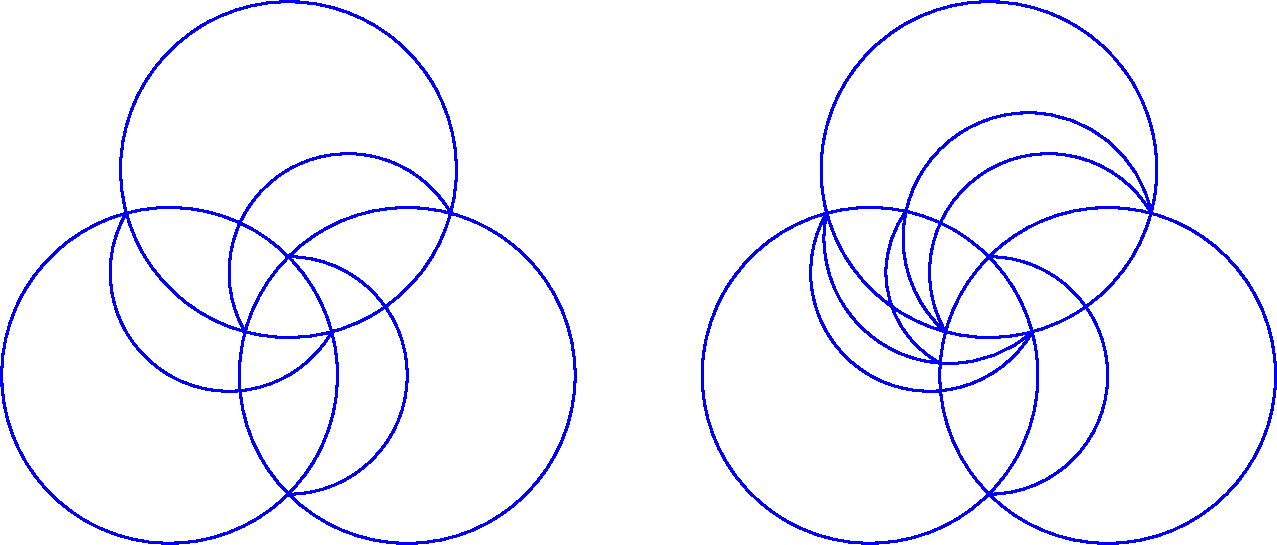
\includegraphics[scale=.45]{clusterFans}}
	\centerline{
	\begin{overpic}[scale=.45]{clusterFans}
	\put(-19,30){$\left[\begin{array}{@{}c@{\;}c@{\;}c@{}} 0 & -1 & 1 \\ 1 & 0 & -1 \\ -1 & 1 & 0 \end{array}\right]$}
	\put(98,30){$\left[\begin{array}{@{}c@{\;}c@{\;}c@{}} 0 & -1 & 2 \\ 1 & 0 & -2 \\ -1 & 1 & 0 \end{array}\right]$}
	\end{overpic}
	}
  \caption{Two $\b{g}$-vector fans~$\gvectorFan[\B_\circ]$ for the type~$A_3$~(left) and type~$C_3$~(right) cyclic initial exchange matrices. As the fans are $3$-dimensional, we intersect them with the sphere and stereographically project them from the direction~$(-1,-1,-1)$. Illustration from~\cite{HohlwegPilaudStella}.}
	\label{fig:clusterFans}
\end{figure}

\begin{theorem}
\label{thm:gvectorFanCA}
For any finite type exchange matrix~$\B_\circ$, the collection of cones \\[.1cm]
\centerline{
$\gvectorFan[\B_\circ] \eqdef \bigset{\R_{\ge0} \, \gvectorsFull{\B_\circ}{\seed}}{\seed \text{ seed of } \principalClusterAlgebra},$
} \\[.1cm]
together with all their faces, forms a complete simplicial fan, called the \defn{$\b{g}$-vector fan} of~$\B_\circ$.
\end{theorem}

Moreover, this fan is known to be polytopal.
More precisely, consider a vector~$\b{h} \in \R^{\variables}$ such that
\[
\b{h}_x + \b{h}_{x'} > \max \Big( \sum_{{y \in \cluster \cap \cluster', \; b_{xy} < 0}} -b_{xy} \, \b{h}_y \;,  \sum_{{y \in \cluster \cap \cluster', \; b_{xy} > 0}} b_{xy} \, \b{h}_y \Big).
\]
for any adjacent seeds~$(\B, \coefficients, \cluster)$ and~$(\B', \coefficients', \cluster')$ with~$\cluster \ssm \{x\} = \cluster' \ssm \{x'\}$.
Such a vector~$\b{h}$ exists, see the discussion in~\cite[Prop.~28]{HohlwegPilaudStella}.

\begin{theorem}[{\cite[Thm.~26]{HohlwegPilaudStella}}]
\label{thm:generalizedAsso}
For any finite type exchange matrix~$\B_\circ$, the $\b{g}$-vector fan~$\gvectorFan[\B_\circ]$ is the normal fan of the \defn{$\B_\circ$-associahedron}~$\Asso[\B_\circ, \b{h}]$ defined equivalently as
\begin{enumerate}[(i)]
\item the convex hull of the points~$\sum_{x \in \seed} \b{h}_x \, \cvectorFull{\B_\circ^\vee}{\seed^\vee}{x^\vee}$ for all seeds~$\seed$ of~$\principalClusterAlgebra$, or
\item the intersection of the halfspaces~$\set{\b{v} \in V^\vee}{\dotprod{\gvectorFull{\B_\circ}{x}}{\b{v}} \le \b{h}_x}$ for all cluster variables~$x$ of~$\principalClusterAlgebra$.
\end{enumerate}
\end{theorem}

\para{Mutations in the $\b{g}$-vector fan}
%
We now discuss the linear dependences between $\b{g}$-vectors of adjacent seeds.
The following proposition was stated in~\cite[Lem.~19]{HohlwegPilaudStella}.

\begin{lemma}
\label{lem:linearDependencegvectorsCA}
For any finite type~exchange matrix~$\B_\circ$ and any adjacent seeds~${(\B, \coefficients, \cluster)}$ and~${(\B', \coefficients', \cluster')}$ in $\principalClusterAlgebra$ with~$\cluster \ssm \{x\} = \cluster' \ssm \{x'\}$, the $\b{g}$-vectors of~$\cluster \cup \cluster'$ with respect to~$\B_\circ$ satisfy precisely one of the following two linear dependences
\[
\gvectorFull{\B_\circ}{x} + \gvectorFull{\B_\circ}{x'} = \sum_{\substack{y \in \cluster \cap \cluster' \\ b_{xy} < 0}} -b_{xy} \, \gvectorFull{\B_\circ}{y}
\quad\text{or}\quad
\gvectorFull{\B_\circ}{x} + \gvectorFull{\B_\circ}{x'} = \sum_{\substack{y \in \cluster \cap \cluster' \\ b_{xy} > 0}} b_{xy} \, \gvectorFull{\B_\circ}{y}.
\]
\end{lemma}

Note that \cref{lem:linearDependencegvectorsCA} implies \cref{thm:generalizedAsso} since it ensures that the type cone~$\typeCone(\gvectorFan[\B_\circ])$ of the $\b{g}$-vector fan contains the cone of~${\b{h} \in \R^{\variables}}$ such that
\(
\b{h}_x + \b{h}_{x'} > \sum_{{y \in \cluster \cap \cluster', \; b_{xy} < 0}} -b_{xy}
\)
and
\(
% \quad\text{and}\quad
\b{h}_x + \b{h}_{x'} > \sum_{{y \in \cluster \cap \cluster', \; b_{xy} > 0}} b_{xy} \, \b{h}_y
\)
for any seeds~$(\B, \coefficients, \cluster)$ and~$(\B', \coefficients', \cluster')$ with~${\cluster \ssm \{x\} = \cluster' \ssm \{x'\}}$.

Unfortunately, \cref{lem:linearDependencegvectorsCA} is less precise than \cref{prop:exchangeablePairsAsso}. Indeed, which of the two possible linear dependences is satisfied by the $\b{g}$-vectors of~$\cluster \cup \cluster'$ depends on the initial exchange matrix~$\B_\circ$.
We will prove however that it is independent of the seeds containing~$x$ and~$x'$.

\begin{proposition}
\label{prop:uniqueExchangePropertyCA}
For any finite type exchange matrix~$\B_\circ$, the $\b{g}$-vector fan has the unique exchange relation property.
\end{proposition}

\subsubsection{Type cone of $\b{g}$-vector fans}

The linear dependences of \cref{lem:linearDependencegvectorsCA} provide a redundant description of the type cone of the $\b{g}$-vector fan~$\gvectorFan[\B_\circ]$.
We denote by~$\b{n}(\B_\circ, x, x')$ the normal vector of the inequality of the type cone corresponding to two exchangeable cluster variable~$x$ to~$x'$ (it is well defined by \cref{prop:uniqueExchangePropertyCA}.
In other words, depending on which of the two linear dependences of \cref{lem:linearDependencegvectorsCA} holds, we have
\[
\b{n}(\B_\circ, x, x') \eqdef \b{f}_x + \b{f}_{x'} - \sum_{\substack{y \in \cluster \cap \cluster' \\ b_{xy} < 0}} -b_{xy} \, \b{f}_y
\qquad\text{or}\qquad
\b{n}(\B_\circ, x, x') \eqdef \b{f}_x + \b{f}_{x'} - \sum_{\substack{y \in \cluster \cap \cluster' \\ b_{xy} > 0}} b_{xy} \, \b{f}_y,
\]
where~$(\b{f}_x)_{x \in \variables}$ denotes the canonical basis of~$\R^{\variables}$.
We obtain the following statement.

\begin{corollary}
\label{coro:typeConeCA}
For any finite type exchange matrix~$\B_\circ$, the type cone of the $\b{g}$-vector fan~$\gvectorFan[\B_\circ]$ is given by
\[
\typeCone(\gvectorFan[\B_\circ]) = \set{\b{h} \in \R^{\variables}}{\dotprod{\b{n}(\B_\circ, x, x')}{\b{h}} > 0 \text{ for all exchangeable cluster variables } x, x'}.
\]
\end{corollary}

In order to describe the facets of this type cone, we need the following special mutations.

\begin{definition}
Consider a seed~$(\B, \coefficients, \cluster)$ and a cluster variable~$x \in \cluster$. The mutation of~$\seed$ in direction~$x$ is a \defn{mesh mutation} if the entries~$b_{xy}$ for~$y \in X$ are all non-negative, or all non-positive.
\end{definition}

For instance, in the initial seed~$(\B_\circ, \coefficients_\circ, \cluster_\circ)$, the mutation in the direction of any variable~${x_\circ \in \cluster_\circ}$ is a mesh.
% and the corresponding $\b{g}$-vector linear dependence is~$\gvectorFull{\B_\circ}{x_\circ} + \gvectorFull{\B_\circ}{x_\circ'} = 0$.
%%, so that~$\b{n}(\B_\circ, x_\circ, x_\circ') = \b{f}_{x_\circ} + \b{f}_{x_\circ'}$. 
We call these meshes \defn{initial}.
The following statement describes the other meshes.

\begin{lemma}
\label{lem:bijectionMeshMutations}
There is precisely one non-initial mesh directed by each positive $\b{c}$-vector of the cluster algebra. Therefore, the number of non-initial meshes is~$N-n$.
\end{lemma}

%The linear dependence among the $\b{g}$-vectors of an initial mesh is just~$\gvectorFull{\B_\circ}{x_\circ} + \gvectorFull{\B_\circ}{x_\circ'} = 0$.
The following statement describes the linear dependence in any other mesh mutation.

\begin{lemma}
Consider two adjacent seeds~${(\B, \coefficients, \cluster)}$ and~${(\B', \coefficients', \cluster')}$ with~$\cluster \ssm \{x\} = \cluster' \ssm \{x'\}$ such that the entries~$b_{xy}$ for~$y \in X$ are all non-positive or all non-negative.
If either~$x$ or~$x'$ is an initial cluster variable, then
\[
\gvectorFull{\B_\circ}{x} + \gvectorFull{\B_\circ}{x'} = 0.
\]
Otherwise, the $\b{g}$-vectors of~$\cluster \cup \cluster'$ with respect to~$\B_\circ$ satisfy the linear dependence
\[
\gvectorFull{\B_\circ}{x} + \gvectorFull{\B_\circ}{x'} = \sum_{y \in \cluster \cap \cluster'} |b_{xy}| \, \gvectorFull{\B_\circ}{y}.
\]
%\[
%\b{n}(\B_\circ, x, x') = \b{f}_x + \b{f}_{x'} - \sum_{y \in \cluster \cap \cluster'} |b_{xy}| \, \b{f}_y
%\]
\end{lemma}

Our main result states that the linear dependences between the $\b{g}$-vectors of any mutation can be decomposed into positive combinations of linear dependences arising from meshes.

\begin{proposition}
\label{prop:extremalExchangeablePairsCA}
\end{proposition}

Our next statement follws from~\cref{prop:extremalExchangeablePairsCA,lem:bijectionMeshMutations}.

\begin{corollary}
\label{coro:simplicialTypeConeCA}
The type cone~$\typeCone(\gvectorFan[n])$ is simplicial.
\end{corollary}

Combining \cref{coro:simplicialTypeCone,coro:simplicialTypeConeCA,prop:extremalExchangeablePairsCA}, we derive the following description of all polytopal realizations of the $\b{g}$-vector fan~$\gvectorFan[\B_\circ]$. This result was stated in~\cite{BazierMatteDouvilleMousavandThomasYildirim} in the special situation of acyclic seeds in simply-laced types.

\begin{theorem}
For any finite type exchange matrix~$\B_\circ$, and for any~$\b{\ell} \in \R_{>0}^{N-n}$, the polytope
\[
R_{\b{\ell}}(\B_\circ) \eqdef \set{\b{z} \in \R^{\variables}}{...}
\]
is a generalized associahedron, whose normal fan is the $\b{g}$-vector fan~$\gvectorFan[\B_\circ]$.
\end{theorem}


\newpage

\begin{remark}
One important observation is that it seems there is one extremal exchangeable pair for each positive $c$-vector, meaning that for each positive $c$-vector~$\beta$, there is precisely one extremal exchangeable pair~$\{x,x'\}$ of cluster variables for which the flip of~$x$ to~$x'$ (for any pair of clusters~$\{X,X'\}$ with~$X \ssm \{x\} = X' \ssm \{x'\}$) is in the direction of~$\beta$.
The goal is thus to determine for each positive root which exchangeable pair is extremal.
This should be done using the Auslander-Reiten quiver to construct two cluster variables from a $c$-vector (see the next paragraph for the idea).
\end{remark}

\newpage

%%%%%%%%%%%

\subsection{Non-kissing complexes and gentle associahedra}

Gentle associahedra were constructed by Y.~Palu, V.~Pilaud and P.-G.~Plamondon~\cite{PaluPilaudPlamondon-nonkissing} in the context of support $\tau$-tilting for gentle algebras.
For a given $\tau$-tilting finite gentle quiver~$\quiver$ (defined in the next section), the $\quiver$-associahedron~$\Asso[\quiver]$ is a simple polytope which encodes certain representations of~$\quiver$ and their $\tau$-tilting relations.
Combinatorially, the $\quiver$-associahedron is a polytopal realization of the non-kissing complex of~$\quiver$, defined as the simplicial complex of all collections of walks on the blossoming quiver~$\quiver\blossom$ which are pairwise non-kissing.
The non-kissing complex encompasses two families of simplicial complexes studied independently in the literature: on the one hand the grid associahedra introduced by T.~K.~Petersen, P.~Pylyavskyy and D.~Speyer in~\cite{PetersenPylyavskyySpeyer} for a staircase shape, studied by F.~Santos, C.~Stump and V.~Welker~\cite{SantosStumpWelker} for rectangular shapes, and extended by T.~McConville in~\cite{McConville} for arbitrary grid shapes; and on the other hand the Stokes polytopes and accordion associahedra studied by Y.~Baryshnikov~\cite{Baryshnikov}, F.~Chapoton~\cite{Chapoton-quadrangulations}, A.~Garver and T.~McConville~\cite{GarverMcConville} and T.~Manneville and V.~Pilaud~\cite{MannevillePilaud-accordion}.
These two families naturally extend the classical associahedron, obtained from a line quiver.
Non-kissing complexes are geometrically realized by polytopes called gentle associahedra, whose normal fan is called the non-kissing fan: its rays correspond to walks in the quiver and its cones are generated by the non-kissing walks.
In this section, we describe the type cone of the non-kissing fan of a quiver~$\quiver$ with no self-kissing walks.

\subsubsection{Non-kissing complex and non-kissing fan of a gentle quiver}

We present the definitions and properties of the non-kissing complex of a gentle quiver, following the presentation of~\cite{PaluPilaudPlamondon-nonkissing}.

\para{Gentle quivers}
%
Consider a \defn{bound quiver}~${\quiver = (Q,I)}$, formed by a finite quiver~$Q = (Q_0, Q_1, s, t)$ and an ideal~$I$ of the path algebra~$kQ$ (the~$k$-vector space generated by all paths in~$Q$, including vertices as paths of length zero, with multiplication induced by concatenation of paths) such that~$I$ is generated by linear combinations of paths of length at least two, and $I$ contains all sufficiently large paths. See~\cite{AssemSimsonSkowronski} for background.

Following M.~Butler and C.~Ringel~\cite{ButlerRingel}, we say that~$\quiver$ is a \defn{gentle bound quiver} when
\begin{enumerate}[(i)]
\item each vertex~$a \in Q_0$ has at most two incoming and two outgoing arrows,
\item the ideal~$I$ is generated by paths of length exactly two,
\item for any arrow~$\beta \in Q_1$, there is at most one arrow~$\alpha \in Q_1$ such that~$t(\alpha) = s(\beta)$ and~${\alpha\beta\notin I}$ (resp.~$\alpha\beta \in I$) and at most one arrow~$\gamma \in Q_1$ such that~$t(\beta) = s(\gamma)$~and~${\beta\gamma\notin I}$~(resp.~${\beta\gamma \in I}$).
\end{enumerate}
The algebra~$kQ/I$ is called a \defn{gentle algebra}.

The \defn{blossoming quiver}~$\quiver\blossom$ of a gentle quiver is the gentle quiver obtained by completing all vertices of~$\quiver$ with additional incoming or outgoing \defn{blossoms} such that all vertices of~$\quiver$ become $4$-valent.
%
%A gentle bound quiver~$\quiver$ is \defn{complete} if any vertex~$a \in Q_0$ is incident to either one ($a$ is a leaf) or four arrows ($a$ is an internal vertex).
%The \defn{pruned subquiver} of a quiver~$\quiver$ is the locally gentle quiver obtained by deleting all leaves of~$\quiver$ (degree one vertices) and their incident arrows.
%The \defn{blossoming quiver} of a locally gentle bound quiver~$\quiver$ is the complete locally gentle bound quiver~$\quiver\blossom$ whose pruned subquiver is~$\quiver$.
%The vertices of~$Q\blossom_0 \ssm Q_0$ are called \defn{blossom vertices}, and the arrows in~$Q\blossom_1 \ssm Q_1$ are called \defn{blossom arrows}.
%
We now always assume that~$\quiver$ is a gentle quiver with blossoming quiver~$\quiver\blossom$.

\para{Strings and walks}
%
A \defn{string} in~$\quiver = (Q,I)$ is a word of the form
\(
\rho = \alpha_1^{\varepsilon_1}\alpha_2^{\varepsilon_2}\cdots \alpha_\ell^{\varepsilon_\ell},
\)
where
	\begin{enumerate}[(i)]
	\item $\alpha_i \in Q_1$ and~$\varepsilon_i \in \{-1,1\}$ for all~$i \in [\ell]$,
	\item $t(\alpha_i^{\varepsilon_i}) = s(\alpha_{i+1}^{\varepsilon_{i+1}})$ for all~$i \in [\ell-1]$,
	\item there is no path~$\pi \in I$ such that~$\pi$ or~$\pi^{-1}$ appears as a factor of~$\rho$, and
	\item $\rho$ is reduced, in the sense that no factor~$\alpha\alpha^{-1}$ or~$\alpha^{-1}\alpha$ appears in~$\rho$, for~$\alpha \in Q_1$.
	\end{enumerate}
%We say that~$\sigma$ is \defn{straight} if~$\varepsilon_1 = \dots = \varepsilon_\ell$.
The integer~$\ell$ is called the \defn{length} of the string~$\rho$.
%We let~$s(\rho) \eqdef s(\alpha_1^{\varepsilon_1})$ and~$t(\rho) \eqdef t(\alpha_\ell^{\varepsilon_\ell})$ denote the source and target of~$\rho$.
For each vertex~$a \in Q_0$, there is also a \defn{string of length zero}, denoted by~$\varepsilon_a$, that starts and ends at~$a$.
We often implicitly identify the two inverse strings~$\rho$ and~$\rho^{-1}$, and call it an \defn{undirected string} of~$\quiver$.
Let~$\strings$ denote the set of strings of~$\quiver$.

A \defn{walk} of~$\quiver$ is a maximal maximal string of its blossoming quiver~$\quiver\blossom$ (meaning that each endpoint is a blossom).
As for strings, we implicitly identify the two inverse walks~$\omega$ and~$\omega^{-1}$, and call it an \defn{undirected walk} of~$\quiver$.
Let~$\walks$ denote the set of walks of~$\quiver$.

A \defn{substring} of a walk~$\omega = \alpha_1^{\varepsilon_1} \cdots \alpha_\ell^{\varepsilon_\ell}$ of~$\quiver$ is a string~$\sigma = \alpha_{i+1}^{\varepsilon_{i+1}} \cdots \alpha_{j-1}^{\varepsilon_{j-1}}$ of~$\quiver$ for some indices~$1 \le i < j \le \ell$. Note that by definition,
\begin{itemize}
\item the endpoints of~$\sigma$ are not allowed to blossom endpoints of~$\omega$,
\item the position of~$\sigma$ as a factor of~$\omega$ matters (the same string at a different position is considered a different substring).
\item the string~$\varepsilon_a$ is a substring of~$\omega$ for each occurence of~$a$ as a vertex of~$\omega$ (take~$j = i+1$).
\end{itemize}
We denote by~$\Sigma(\omega)$ the set of substrings of~$\omega$.
We say that the substring~$\sigma = \alpha_{i+1}^{\varepsilon_{i+1}} \cdots \alpha_{j-1}^{\varepsilon_{j-1}}$ is \defn{at the bottom} (resp.~\defn{on top}) of the walk~$\omega = \alpha_1^{\varepsilon_1} \cdots \alpha_\ell^{\varepsilon_\ell}$ if~$\varepsilon_i = 1$ and~$\varepsilon_j = -1$ (resp.~if~$\varepsilon_i = -1$ and~$\varepsilon_j = 1$).
In other words the two arrows of~$\omega$ incident to the endpoints of~$\sigma$ point towards~$\sigma$ (resp.~outwards from~$\sigma$).
We denote by~$\Sigma_\bottom(\omega)$ and~$\Sigma_\top(\omega)$ the sets of bottom and top substrings of~$\omega$ respectively.
We use the same notation for undirected walks (of course, substrings of an undirected walk are undirected).

A \defn{peak} (resp.~\defn{deep}) of a walk~$\omega$ is a substring of~$\omega$ of length zero which is on top (resp.~at the bottom of~$\omega$).
A walk~$\omega$ is \defn{straight} if it has no peak or deep (\ie if~$\omega$ or~$\omega^{-1}$ is a path in~$\quiver\blossom$), and \defn{bending} otherwise.
We denote by~$\peaks{\omega}$ (resp.~$\deeps{\omega}$) the multisets of vertices of peaks (resp.~deeps) of~$\omega$.

\para{Non-kissing complex}
%
Let~$\omega$ and~$\omega'$ be two undirected walks on~$\quiver$.
We say that~$\omega$ \defn{kisses}~$\omega'$ if ${\Sigma_\top(\omega) \cap \Sigma_\bottom(\omega')} \ne \varnothing$.
In other words, $\omega$ and~$\omega'$ share a common substring~$\sigma$, and both arrows of~$\omega$ (resp.~of~$\omega'$) not in~$\sigma$ are outgoing (resp.~incoming) at the endpoints of~$\sigma$.
%See \fref{fig:kissing}.
We say that~$\omega$ and~$\omega'$ are \defn{kissing} if~$\omega$ kisses~$\omega'$ or~$\omega'$ kisses~$\omega$ (or both).
Note that we authorize the situation where the common finite substring is reduced to a vertex~$a$, that~$\omega$ can kiss~$\omega'$ several times, that~$\omega$ and~$\omega'$ can mutually kiss, and that~$\omega$ can kiss itself.
We say that a walk is \defn{proper} if it is not straight nor self-kissing.
We denote by~$\properWalks$ the set of all proper walks of~$\quiver$.

%\begin{figure}[h]
%	\capstart
%	\centerline{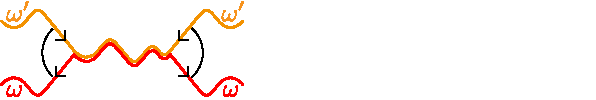
\includegraphics[scale=1]{kissing}}
%	\caption{A schematic representation of two kissing walks: $\omega$~kisses~$\omega'$.}
%	\label{fig:kissing}
%\end{figure}
%
The (reduced) \defn{non-kissing complex} of~$\quiver$ is the simplicial complex~$\NKC$ whose faces are the collections of pairwise non-kissing proper walks of~$\quiver$.
As shown in~\cite[Thm.~2.46]{PaluPilaudPlamondon-nonkissing}, this simplicial complex is a combinatorial model for the support $\tau$-tilting complex on $\tau$-rigid modules over~$kQ/I$.
The quiver~$\quiver$ is called \defn{$\tau$-tilting finite} or \defn{non-kissing finite} when this complex is finite (in other words, $\quiver$ has finitely may non-kissing walks).

\para{$\b{g}$- and $\b{c}$-vectors}
%
We now define two families of vectors associated to walks in the non-kissing complex.
Let~$(\b{e}_v)_{v \in Q_0}$ denote the canonical basis of~$\R^{Q_0}$.
For a multiset~$V = \{\!\{v_1, \dots, v_k\}\!\}$ of~$Q_0$, we denote by $\multiplicityVector_V \eqdef \sum_{i \in [k]} \b{e}_{v_i}$.

\begin{definition}[{\cite[Def.~{4.8}]{PaluPilaudPlamondon-nonkissing}}]
The \defn{$\b{g}$-vector} of a walk~$\omega$ is~$\gvector{\omega} \eqdef \multiplicityVector_{\peaks{\omega}} - \multiplicityVector_{\deeps{\omega}}$.
We denote by~$\gvectors{F} \eqdef \set{\gvector{\omega}}{\omega \in F}$ the set of $\b{g}$-vectors of a facet~$F$.
\end{definition}

Note that by definition, the $\gvector{\omega} = 0$ for a straight walk~$\omega$.

To define the other family of vectors, we need to recall the notion of distinguished substring of a walk defined in~\cite[Def.~2.25]{PaluPilaudPlamondon-nonkissing}.
Consider an arrow~$\alpha \in Q_1$ contained in two distinct walks~$\omega, \omega'$ of a non-kissing facet~$F \in \NKC$, and let~$\sigma$ denote the common substring of~$\omega$ and~$\omega'$.
We write~$\omega \prec_\alpha \omega'$ if $\omega$ enters and/or exits~$\sigma$ with arrows in the direction pointed by~$\alpha$, while $\omega'$ enters and/or exits~$\sigma$ with arrows in the direction opposite to~$\alpha$.
The \defn{distinguished walk} of the non-kissing facet~$F \in \NKC$ at the arrow~$\alpha$ is the maximum walk of~$F$ for~$\prec_\alpha$.
The \defn{distinguished arrows} of the walk~$\omega$ in the non-kissing facet~$F \in \NKC$ are the arrow where~$\omega$ is the distinguished walk.
It is shown in~\cite[Prop.~2.28]{PaluPilaudPlamondon-nonkissing} that each bending walk in a non-kissing facet has precisely two distinguished arrows, pointing in opposite directions.
The \defn{distinguished substring}~$\distinguishedString{\omega}{F}$ of the walk~$\omega$ in the non-kissing facet~$F \in \NKC$ is the substring located between its two distinguished arrows.

\begin{definition}[{\cite[Def.~{4.11}]{PaluPilaudPlamondon-nonkissing}}]
The \defn{$\b{c}$-vector} of a walk~$\omega$ in a non-kissing facet~${F \in \NKC}$ is~${\cvector{F}{\omega} \eqdef \distinguishedSign{\omega}{F} \, \multiplicityVector_{\distinguishedString{\omega}{F}}}$, where~$\distinguishedSign{\omega}{F} \in \{-1,1\}$ is positive if~${\distinguishedString{\omega}{F} \in \Sigma_\top(\omega)}$ and negative if~${\distinguishedString{\omega}{F} \in \Sigma_\bottom(\omega)}$.
We denote by~$\cvectors{F} \eqdef \set{\cvector{F}{\omega}}{\omega \in F}$ the set of $\b{c}$-vectors~of~a~facet~$F$.
\end{definition}

The $\b{g}$- and $\b{c}$-vectors also form dual bases.

\begin{proposition}
\label{prop:gvectorscvectorsDualBasesGentle}
For any non-kissing facet~$F \in \NKC$, the set of $\b{g}$-vectors~$\gvectors{F}$ and the set of $\b{c}$-vectors~$\cvectors{F}$ form dual bases, that is
\(
{\bigdotprod{\gvector{\omega}}{\cvector{F}{\omega'}} = \delta_{\omega=\omega'}}
\)
for any two walks~$\omega, \omega' \in F$.
\end{proposition}

\para{Non-kissing fan and gentle associahedron}
%
The $\b{g}$-vectors support a complete simplicial fan realization of the non-kissing complex complex.
Examples are illustrated in \cref{fig:nonkissingFans}.

\begin{figure}[h]
	\capstart
	\centerline{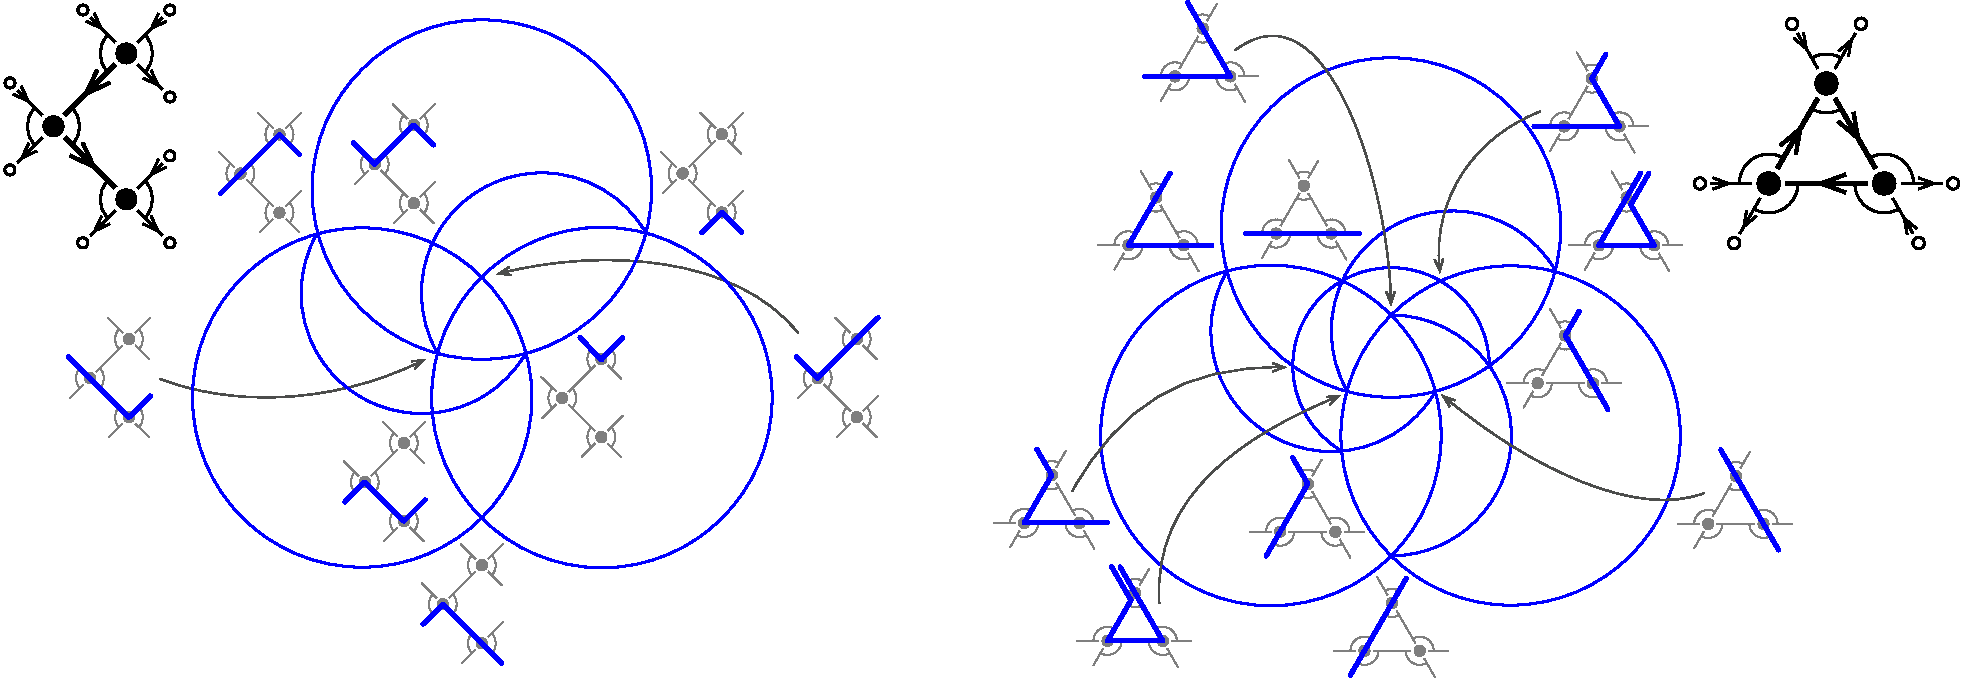
\includegraphics[scale=.45]{nonkissingFans}}
	\caption{Two non-kissing fans. As the fans are $3$-dimensional, we intersect them with the sphere and stereographically project them from the direction~$(-1,-1,-1)$. Illustration from~\cite{PaluPilaudPlamondon-nonkissing}.}
	\label{fig:nonkissingFans}
\end{figure}

\begin{theorem}[{\cite[Thm.~4.17]{PaluPilaudPlamondon-nonkissing}}]
\label{thm:nonkissingAsso}
For any non-kissing finite gentle quiver~$\quiver$, the set of cones
\[
\gvectorFan[\quiver] \eqdef \set{\R_{\ge 0} \, \gvectors{F}}{F \text{ non-kissing face of } \NKC}
\]
is a complete simplicial fan of~$\R^{Q_0}$, called \defn{non-kissing fan} of~$\quiver$, which realizes the non-kissing complex~$\NKC$.
\end{theorem}

It is proved in~\cite[Thm.~4.27]{PaluPilaudPlamondon-nonkissing} that the non-kissing fan comes from a polytope.
For a walk~$\omega$, denote by~$\KN(\omega)$ the sum over all other walks~$\omega'$ of the number of kisses between~$\omega$~and~$\omega'$.

\begin{theorem}[{\cite[Thm.~4.27]{PaluPilaudPlamondon-nonkissing}}]
For any non-kissing finite gentle quiver~$\quiver$, the non-kissing fan~$\gvectorFan[\quiver]$ is the normal fan of the \defn{gentle associahedron}~$\Asso[\quiver]$ defined equivalently as:
\begin{enumerate}[(i)]
\item the convex hull of the points~$\sum_{\omega \in F} \KN(\omega) \, \cvector{F}{\omega}$ for all facets~${F \in \NKC}$,~or
\item the intersection of the halfspaces~$\bigset{\b{x} \in \R^{Q_0}}{\dotprod{\gvector{\omega}}{\b{x}} \le \KN(\omega)}$ for all walks~$\omega$ on~$\bar Q$.
\end{enumerate}
\end{theorem}

\para{Flips in the non-kissing fan}
%
Although we lack a characterization of the exchangeable pairs of the non-kissing complex (see \cref{rem:exchangeablePairsNKC}), we can still describe the linear dependence among the $\b{g}$-vectors involved in a flip.
The following statement is partially proved in~\cite[Thm.~4.17]{PaluPilaudPlamondon-nonkissing}.

\begin{proposition}
\label{prop:exchangeablePairsNKC}
Let~$\omega, \omega'$ be two exchangeable walks on~$\quiver$. Then
\begin{enumerate}[(i)]
\item For any non-kissing facet~$F, F'$ of~$\NKC$ with~$F \ssm \{\omega\} = f' \ssm \{\omega'\}$, there exists a unique maximal common substring~$\sigma$ of~$\omega$ and~$\omega'$ that decomposes~$\omega = \rho \sigma \tau$ and~$\omega' = \rho' \sigma \tau'$ such that the facets~$F$ and~$F'$ both contain the walks~$\mu \eqdef \rho' \sigma \tau$ and~$\nu \eqdef \rho \sigma \tau'$.
\item The substring~$\sigma$ and thus the walks~$\mu$ and~$\nu$ actually depend on the exchangeable walks~$\omega$ and~$\omega'$, not on the adjacent non-kissing facet~$F $ and~$F'$.
\item Moreover, the linear dependence between the $\b{g}$-vectors of~$F \cup F'$ is given by
\[
\gvector{\omega} + \gvector{\omega'} = \gvector{\mu} + \gvector{\nu}.
\]
In other words, the non-kissing fan of~$\quiver$ has the unique exchange relation property.
\item The $\b{c}$-vector orthogonal to all $\b{g}$-vectors~$\gvector{\lambda}$ for~$\lambda \in F \cap F'$ is the multiplicity vector~$\multiplicityVector_{\sigma}$ of the vertices of the substring~$\sigma$ of~$\omega$ and~$\omega'$.
\end{enumerate}
\end{proposition}

\begin{proof}
Points~(i), (iii) and~(iv) where shown in~\cite[Prop.~2.33, Thm.~4.17 \& Prop~4.16]{PaluPilaudPlamondon-nonkissing}.
\vincent{Point~(ii) to prove.}
\end{proof}

In \cref{prop:exchangeablePairsNKC}, the string~$\sigma$ is called the \defn{distinguished} substring of~$\omega$ and~$\omega'$.
We say that a string~$\sigma$ is \defn{distinguishable} if it is the distinguished string of an exchangeable pair.
Note that an equivalent definition of distinguishable strings is given in~\cite[Def.~2.30]{PaluPilaudPlamondon-nonkissing}.
We denote by~$\distinguishableStrings$ the set of distinguishable strings of~$\quiver$.
\vincent{Clean that}

\begin{remark}
\label{rem:exchangeablePairsNKC}
In view of \cref{prop:exchangeablePairsNKC}, it is tempting to look for a characterization of the exchangeable pairs~$\omega, \omega'$ using the kisses between~$\omega$ and~$\omega'$.
However, as illustrated in \cref{fig:nonkissingFans}\,(right), note that
\begin{itemize}
\item two exchangeable walks may kiss along more than one string, but only one is the distinguished string,
\item two non-exchangeable walks can kiss along more than one distinguishable string,
\item two walks that kiss along a single distinguishable string are not always exchangeable,
\item not all strings are distinguishable.
\end{itemize}
\vincent{More explicit. TODO}
\vincent{Do we still have these problems when the gentle algebra is brick and/or without oriented $2$-cycle?}
\end{remark}

\begin{corollary}
For any non-kissing finite gentle quiver~$\quiver$, the type cone of the non-kissing fan~$\gvectorFan[\quiver]$ is given by
\[
\typeCone(\gvectorFan[\quiver]) = \set{\b{h} \in \R^{\walks}}{\begin{array}{l} \b{h}_\omega = 0 \text{ for any improper walk } \omega \\ \b{h}_\omega + \b{h}_{\omega'} > \b{h}_\mu + \b{h}_\nu \text{ for any exchangeable walks } \omega, \omega' \end{array}}.
\]
\end{corollary}

\para{Numerology}
%
The following result will also be essential in our discussion.

\begin{proposition}[{\cite[3.68]{PaluPilaudPlamondon-nonkissing}}]
\label{prop:bijectionStringsWalks}
The number of distinguishable strings~$\distinguishableStrings$ and proper walks~$\properWalks$ of the quiver~$\quiver$ are related by
\[
|\distinguishableStrings| + |Q_0| = |\properWalks|.
\]
\end{proposition}

\para{Two families of examples: grid and dissection quivers}
%
We conclude this recollections on non-kissing complexes by two families of examples.
\vincent{TODO}

\bigskip
We are now ready to describe the type cone of the non-kissing fan~$\gvectorFan[\quiver]$.
We first treat the case when~$\quiver$ has no self-kissing walks, which includes both grid and dissection quivers, thus in particular the case of the classical associahedron.
We show that the type cone is then simplicial which gives another proof of \cref{thm:simplicialTypeConeAsso} and \cref{coro:descriptionAllAsso}.

\subsubsection{Simplicial type cones for self-kissing free quivers}

In this section, we focus on the following family of gentle quivers, which was also considered in~\cite[Sect.~4]{}.

\begin{proposition}
\label{prop:noSelfKissing}
The following conditions are equivalent for a gentle quiver~$\quiver$.
\begin{enumerate}[(i)]
\item any (non necessarily oriented) cycle of~$\quiver$ contains at least two relations in~$I$,
\item any string of~$\quiver$ is distinguishable,
\item no walk on~$\quiver$ is self-kissing.
\end{enumerate}
\end{proposition}

The quivers of this family are particularly well-behaved: they avoid all pathologies of \cref{rem:exchangeablePairsNKC} and we will prove that the type cone of their non-kissing fan happens to be simplicial.\pg{Need to exclude two-cycles, else false.}
Note that this family already contains a lot of relevant examples, including:
\begin{itemize}
\item classical associahedra
\item grid associahedra
\item dissection associahedra
\end{itemize}
\vincent{More explicit. TODO}

%For a string~$\sigma$ of~$\quiver$, we denote by $\sigma\hR$ (resp.~$\hL\sigma$, resp.~$\sigma\cR$, resp.~$\cL\sigma$) the unique string of~$\quiver\blossom$ of the form $\sigma\hR = \sigma \alpha_1^{-1} \alpha_2 \dots \alpha_\ell$ (resp.~$\hL\sigma = \alpha_\ell^{-1} \dots \alpha_2^{-1} \alpha_1 \sigma$, resp.~$\sigma\cR = \sigma \alpha_1 \alpha_2^{-1} \dots \alpha_\ell^{-1}$, resp.~$\cL\sigma = \alpha_\ell \dots \alpha_2 \alpha_1^{-1} \sigma$) with~$\ell \ge 1$ and~$\alpha_1, \dots, \alpha_\ell \in Q_1$ and such that~$t(\alpha_\ell)$ (resp.~$s(\alpha_\ell)$, resp.~$s(\alpha_\ell)$, resp.~$t(\alpha_\ell)$) is a blossom of~$\quiver\blossom$.
For a string~$\sigma$ of~$\quiver$, we denote by $\sigma\hR$ (resp.~$\sigma\cR$) the unique string of the blossoming quiver~$\quiver\blossom$ of the form $\sigma\hR = \sigma \alpha_1^{-1} \alpha_2 \dots \alpha_\ell$ (resp.~$\sigma\cR = \sigma \alpha_1 \alpha_2^{-1} \dots \alpha_\ell^{-1}$) with~$\ell \ge 1$ and~${\alpha_1, \dots, \alpha_\ell \in Q_1}$ and such that~$t(\alpha_\ell)$ (resp.~$s(\alpha_\ell)$) is a blossom of~$\quiver\blossom$.
These notations are motivated by the representation of strings used in~\cite{ButlerRingel, PaluPilaudPlamondon-nonkissing}, and the terminology usually says that~$\sigma\hR$ (resp.~$\sigma\cR$) is obtained by adding a \defn{hook} (resp.~\defn{cohook}) to~$\sigma$.
We define similarly~$\hL\sigma$ (resp.~$\cL\sigma$).
The walk~$\hL(\sigma\hR) = (\hL\sigma)\hR$ of~$\quiver$ is simply be denoted~$\hh{\sigma}$, and we define similarly~$\cc{\sigma}$, $\hc{\sigma}$ and~$\ch{\sigma}$.

%For a string~$\sigma$ of~$\quiver$, we denote by~$\hh{\sigma}$, $\cc{\sigma}$, $\hc{\sigma}$ and~$\ch{\sigma}$ the unique walks on~$\quiver$ of the~form
%\begin{alignat*}{3}
%\hh{\sigma} & = \alpha_k^{-1} \dots \alpha_2^{-1} \alpha_1 \sigma \beta_1^{-1} \beta_2 \dots \beta_\ell
%\qquad\qquad
%& \cc{\sigma} & = \alpha_k \dots \alpha_2 \alpha_1^{-1} \sigma \beta_1 \beta_2^{-1} \dots \beta_\ell^{-1}
%\\
%\hc{\sigma} & = \alpha_k^{-1} \dots \alpha_2^{-1} \alpha_1 \sigma \beta_1 \beta_2^{-1} \dots \beta_\ell^{-1}
%\qquad\qquad
%& \ch{\sigma} & = \alpha_k \dots \alpha_2 \alpha_1^{-1} \sigma \beta_1^{-1} \beta_2 \dots \beta_\ell.
%\end{alignat*}
%%\begin{itemize}
%%\item by~$\hh{\sigma}$ the unique walk on~$\quiver$ of the form~$\hh{\sigma} = \alpha_k^{-1} \dots \alpha_2^{-1} \alpha_1 \sigma \beta_1^{-1} \beta_2 \dots \beta_\ell$,
%%\item by~$\cc{\sigma}$ the unique walk on~$\quiver$ of the form~$\cc{\sigma} = \alpha_k \dots \alpha_2 \alpha_1^{-1} \sigma \beta_1 \beta_2^{-1} \dots \beta_\ell^{-1}$.
%%\item by~$\hc{\sigma}$ the unique walk on~$\quiver$ of the form~$\hc{\sigma} = \alpha_k^{-1} \dots \alpha_2^{-1} \alpha_1 \sigma \beta_1 \beta_2^{-1} \dots \beta_\ell^{-1}$.
%%\item by~$\ch{\sigma}$ the unique walk on~$\quiver$ of the form~$\ch{\sigma} = \alpha_k \dots \alpha_2 \alpha_1^{-1} \sigma \beta_1^{-1} \beta_2 \dots \beta_\ell$.
%%\end{itemize}
%with~$k,\ell \ge 1$ and~$\alpha_1, \dots, \alpha_k, \beta_1, \dots, \beta_\ell \in Q_1$.
%The following statement ensures that in a gentle quiver with no self-kissing walk, the walks~$\hh{\sigma}$ and~$\cc{\sigma}$ are exchangeable with distinguished substring~$\sigma$.

\begin{proposition}
For any gentle quiver~$\quiver$ with no self-kissing walk and any string~$\sigma \in \strings$, the walks~$\cc{\sigma}$ and~$\hh{\sigma}$ are exchangeable with distinguished substring~$\sigma$.
\vincent{This is FALSE...}
\end{proposition}

\begin{proof}
We just need to prove that there exists a ridge~$R$ of~$\NKC$ containing both~$\hc{\sigma}$ and~$\ch{\sigma}$ and such that~$R \cup \{\cc{\sigma}\}$ and~$R \cup \{\hh{\sigma}\}$ are adjacent facets of~$\NKC$.
\vincent{TODO}
\end{proof}

The following statement describes the type cone of the non-kissing fan of a gentle quiver with no self-kissing walks.

\begin{proposition}
\label{prop:extremalExchangeablePairsNKC}
For any gentle quiver~$\quiver$ with no self-kissing walk, the extremal exchangeable pairs for the non-kissing fan of~$\quiver$ are precisely the pairs~$\{\cc{\sigma}, \hh{\sigma}\}$ for all strings~$\sigma \in \strings$.
\end{proposition}

\begin{proof}
Let~$(\b{f}_\omega)_{\omega \in \walks}$ be the canonical basis of~$\R^{\walks}$.
Consider two exchangeable walks~$\omega$ and~$\omega'$ with distinguished substring~$\sigma \in \Sigma_\top(\omega) \cap \Sigma_\bottom(\omega')$.
Decompose~$\omega = \rho \sigma \tau$ and~$\omega' = \rho' \sigma \tau'$ and define~$\mu \eqdef \rho' \sigma \tau$ and~$\nu \eqdef \rho \sigma \tau'$ as in \cref{prop:exchangeablePairsNKC}\,(i). \cref{prop:exchangeablePairsNKC}\,(iii) ensures that the linear dependence between the corresponding $\b{g}$-vectors is given by
\[
\gvector{\omega} + \gvector{\omega'} = \gvector{\mu} + \gvector{\nu}.
\]
Therefore, the outer normal vector of the corresponding inequality of the type cone~$\typeCone(\gvectorFan[\quiver])$ is
\[
\b{n}(\omega, \omega') \eqdef \b{f}_\omega + \b{f}_{\omega'} - \b{f}_\mu - \b{f}_\nu.
\]
We claim that this normal vector is always a positive linear combination of the normal vectors~$\b{m}(\sigma) \eqdef \b{n}(\cc{\sigma}, \hh{\sigma}) = \b{f}_{\cc{\sigma}} + \b{f}_{\hh{\sigma}} - \b{f}_{\hc{\sigma}} - \b{f}_{\ch{\sigma}}$ for all string~$\sigma \in \strings$.
Our proof works by descending induction on the length~$\lambda(\omega,\omega') \eqdef \ell(\sigma)$ of the common substring of~$\omega$ and~$\omega'$.
If~$\lambda(\omega, \omega')$ is big enough, then the walk~$\omega$ (resp.~$\omega'$) is just obtained by adding two outgoing (resp.~incoming) blossoms at the end of~$\sigma$, thus $\omega = \cc{\sigma}$ (resp.~$\omega' = \hh{\sigma}$), and there is nothing to prove.
Assume now that~$\omega \ne \hh{\sigma}$ (the situations where~$\omega' \ne \cc{\sigma}$ or~$\omega \ne \rho \sigma \hR$ are symmetric).
%Assume now that~$\omega \ne \hh{\sigma}$, for instance that~$\omega \ne \hL \sigma \tau$ (the situations where~$\omega' \ne \cc{\sigma}$ or~$\omega \ne \rho \sigma \hR$ are symmetric).
%Let~$\xi \eqdef \hL \sigma \tau$ and $\zeta \eqdef \hL \sigma \tau'$.
%These notations are summarized in \cref{fig:proofExtremalExchangeablePairsNKC}.
If~$\rho \ne \cL$, observe that
\begin{itemize}
\item $\omega$ and~$\cL \sigma \tau'$ are exchangeable with~$\b{n}(\omega, \cL \sigma \tau') = \b{f}_\omega + \b{f}_{\cL \sigma \tau'} - \b{f}_{\cL \sigma \tau} - \b{f}_\nu$, and
\item $\cL \sigma \tau$ and~$\omega'$ are exchangeable with~$\b{n}(\cL \sigma \tau, \omega') = \b{f}_{\cL \sigma \tau} + \b{f}_{\omega'} - \b{f}_{\cL \sigma \tau'} - \b{f}_\mu$.
\end{itemize}
We derive that
\[
\b{n}(\omega, \omega') = \b{n}(\omega, \cL \sigma \tau') + \b{n}(\cL \sigma \tau, \omega').
\]
Observe moreover that since~$\omega$ has outgoing arrows at the endpoints of~$\sigma$, the common substring of~$\omega$ and~$\cL \sigma \tau'$ strictly contains~$\sigma$ so that $\lambda(\omega, \cL \sigma \tau') > \lambda(\omega, \omega')$.
By induction, $\b{n}(\omega, \cL \sigma \tau')$ is thus a positive linear combination of~$\b{m}(\sigma)$ for~$\sigma \in \strings$.
%
By symmetry, we obtain the four equalities
\[
\b{n}(\omega, \omega') = 
\begin{cases}
\b{n}(\omega, \cL \sigma \tau') + \b{n}(\cL \sigma \tau, \omega') & \text{if } \rho \ne \cL, \\
\b{n}(\omega, \rho' \sigma \cR) + \b{n}(\rho \sigma \cR, \omega') & \text{if } \tau \ne \cR, \\
\b{n}(\omega, \hL \sigma \tau') + \b{n}(\hL \sigma \tau, \omega') & \text{if } \rho' \ne \hL, \\
\b{n}(\omega, \rho' \sigma \hR) + \b{n}(\rho \sigma \hR, \omega') & \text{if } \tau' \ne \hR.
\end{cases}
\]
These four equalities are illustrated on \cref{fig:fourEqualities}.
%
\begin{figure}[t]
	\capstart
%	\centerline{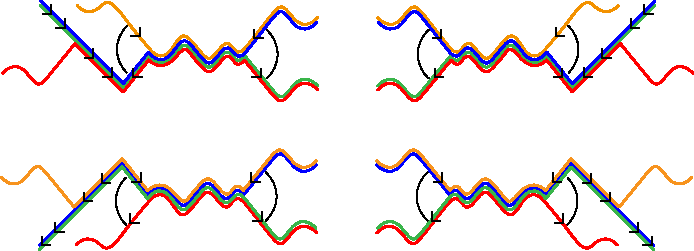
\includegraphics[scale=1.2]{fourEqualities}}
	\centerline{
	\begin{tabular}{c@{\qquad}c}
		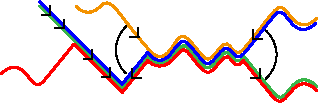
\includegraphics[scale=1.2]{fourEqualities1} & 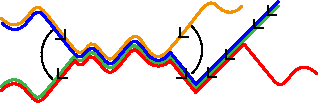
\includegraphics[scale=1.2]{fourEqualities2} \\
		$\b{n}({\red \omega}, {\orange \omega'}) = \b{n}({\red \omega}, {\blue \cL \sigma \tau'}) + \b{n}({\green \cL \sigma \tau}, {\orange \omega'})$ & $\b{n}({\red \omega}, {\orange \omega'}) = \b{n}({\red \omega}, {\blue \rho' \sigma \cR}) + \b{n}({\green \rho \sigma \cR}, {\orange \omega'})$ \\[.4cm]
		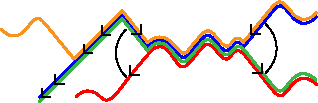
\includegraphics[scale=1.2]{fourEqualities3} & 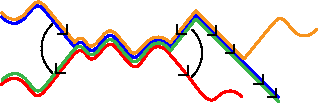
\includegraphics[scale=1.2]{fourEqualities4} \\
		$\b{n}({\red \omega}, {\orange \omega'}) = \b{n}({\red \omega}, {\blue \hL \sigma \tau'}) + \b{n}({\green \hL \sigma \tau}, {\orange \omega'})$ & $\b{n}({\red \omega}, {\orange \omega'}) = \b{n}({\red \omega}, {\blue \rho' \sigma \hR}) + \b{n}({\green \rho \sigma \hR}, {\orange \omega'})$ \\
	\end{tabular}
	}
	\caption{Schematic representation of te four equalities in the proof of \cref{prop:extremalExchangeablePairsNKC}.}
	\label{fig:fourEqualities}
\end{figure}
%
Moreover~$\b{n}(\omega, \cL \sigma \tau')$, $\b{n}(\cL \sigma \tau, \hL \sigma \cR)$, $\b{n}(\cL \sigma \hR, \hL \sigma \tau')$ and~$\b{n}(\hL \sigma \tau, \omega')$ are all positive combinations of~$\b{m}(\sigma)$ for~$\sigma \in \strings$ by induction hypothesis.
%
Applying these equalities one after the other, we obtain
\[
\renewcommand{\arraystretch}{1.3}
\begin{array}[t]{l@{\;\;}l@{\;}l@{\;}l@{\;}l@{\;}l@{\;}l@{\;}l@{\;}l@{\;}l}
  & \b{n}(\omega, \omega') & & \hfill\raisebox{-.1cm}{\text{\tiny{Equality 1}}} & & & & & & \\
\cline{2-4}
= & \b{n}(\omega, \cL \sigma \tau') & + & \b{n}(\cL \sigma \tau, \omega') & & & & & & \hfill\raisebox{-.1cm}{\text{\tiny{Equality 2}}} \\
\cline{4-10}
= & \b{n}(\omega, \cL \sigma \tau') & + & \b{n}(\cL \sigma \tau, \hL \sigma \tau') & & \hfill\raisebox{-.1cm}{\text{\tiny{Equality 3}}} & & & + & \b{n}(\hL \sigma \tau, \omega') \\
\cline{4-6}
= & \b{n}(\omega, \cL \sigma \tau') & + & \b{n}(\cL \sigma \tau, \hL \sigma \cR) & + & \b{n}(\cL \sigma \cR, \hL \sigma \tau') & & \hfill\raisebox{-.1cm}{\text{\tiny{Equality 4}}} & + & \b{n}(\hL \sigma \tau, \omega') \\
\cline{6-8}
= & \b{n}(\omega, \cL \sigma \tau') & + & \b{n}(\cL \sigma \tau, \hL \sigma \cR) & + & \b{n}(\cL \sigma \cR, \hL \sigma \hR) & + & \b{n}(\cL \sigma \hR, \hL \sigma \tau') & + & \b{n}(\hL \sigma \tau, \omega') \\
= & \b{n}(\omega, \cL \sigma \tau') & + & \b{n}(\cL \sigma \tau, \hL \sigma \cR) & + & \multicolumn{1}{c}{\b{m}(\sigma)} & + & \b{n}(\cL \sigma \hR, \hL \sigma \tau') & + & \b{n}(\hL \sigma \tau, \omega')
\end{array}
\renewcommand{\arraystretch}{1}
\]
where we fix the convention~$\b{n}(\lambda, \lambda) = 0$ in case~$\rho = \hL$, $\rho' = \cL$, $\tau = \hR$ or~$\tau' = \cR$.
%
We conclude that~$\b{n}(\omega, \omega')$ is a positive combination of~$\b{m}(\sigma)$ for~$\sigma \in \strings$, since~$\b{n}(\omega, \cL \sigma \tau')$, $\b{n}(\cL \sigma \tau, \hL \sigma \cR)$, $\b{n}(\cL \sigma \hR, \hL \sigma \tau')$ and~$\b{n}(\hL \sigma \tau, \omega')$ are.
This shows that all extremal exchangeable pairs are of the form~$\{\cc{\sigma}, \hh{\sigma}\}$ for~$\sigma \in \strings$.

Conversely, we know from \cref{rem:dimTypeCone} that there are at least~$|\properWalks|-|Q_0|$ extremal exchangeable pairs. Since this~$|\strings| = |\distinguishableStrings| = |\properWalks| - |Q_0|$ by~\cref{prop:bijectionStringsWalks}, we conclude that all exchangeable pairs~$\{\cc{\sigma}, \hh{\sigma}\}$ for~$\sigma \in \strings$ are extremal.
\end{proof}

The following statement now follows from \cref{prop:bijectionStringsWalks,prop:extremalExchangeablePairsNKC}.

\begin{corollary}
\label{coro:simplicialTypeConeNKC}
For any gentle quiver~$\quiver$ with no self-kissing walk, the type cone~$\typeCone(\gvectorFan[\quiver])$ of the non-kissing fan~$\quiver$ is simplicial.
\end{corollary}

Combining \cref{coro:simplicialTypeCone}, \cref{coro:simplicialTypeConeNKC} and \cref{prop:extremalExchangeablePairsNKC}, we derive the following description of all polytopal realizations of the non-kissing fan~$\gvectorFan[\quiver]$ of a quiver~$\quiver$ with no self-kissing~walk.

\begin{corollary}
For any gentle quiver~$\quiver$ with no self-kissing walk and any~$\b{\ell} \in \R_{>0}^{\strings}$, the polytope
\[
R_\b{\ell}(\quiver) \eqdef \set{\b{z} \in \R^{\walks}}{\begin{array}{l} \b{z} \ge 0 \qquad\text{and}\qquad \b{z}_\omega = 0 \text{ for any improper walk } \omega \\ \b{z}_{\cc{\sigma}} + \b{z}_{\hh{\sigma}} - \b{z}_{\hc{\sigma}} - \b{z}_{\ch{\sigma}} = \b{\ell}_\sigma \text{ for all } \sigma \in \strings\end{array}}
\]
is a realization of the non-kissing fan~$\gvectorFan[\quiver]$.
Moreover, the polytopes~$R_\b{\ell}(\quiver)$ for~$\b{\ell} \in \R_{>0}^{\strings}$ describe all polytopal realizations of~$\gvectorFan[\quiver]$.
\end{corollary}

\begin{proof}
\cref{prop:extremalExchangeablePairsNKC} asserts that the type cone~$\typeCone(\gvectorFan[\quiver])$ has one facet for each string of~$\quiver$.
Since all strings are distinguishable by \cref{prop:noSelfKissing}, the number of facets of~$\typeCone(\gvectorFan[\quiver])$ is $|\strings| = |\distinguishableStrings| = |\properWalks| - |Q_0|$ by~\cref{prop:bijectionStringsWalks}, so that~$\typeCone(\gvectorFan[\quiver])$ is simplicial. We then conclude by a simple application of \cref{coro:simplicialTypeCone}.
\end{proof}

We also obtain from \cref{prop:extremalExchangeablePairsNKC} the following surprising property.

\begin{corollary}
Any $\b{c}$-vector supports exactly one extremal exchangeable pair.
\end{corollary}

\begin{remark}
\label{rem:meshARquiver}
Although not needed in the proof of \cref{prop:extremalExchangeablePairsNKC}, we note that the extremal exchangeable pairs~$\{\cc{\sigma}, \hh{\sigma}\}$ and their linear dependencies~${\gvector{\cc{\sigma}} + \gvector{\hh{\sigma}} - \gvector{\hc{\sigma}} - \gvector{\ch{\sigma}}}$ precisely correspond to the meshes of the Auslander-Reiten quiver of~$\quiver$.
\end{remark}

\subsubsection{Towards the general case}

We are already missing a criterion for exchangeable pairs of walks. See \cite[Sect.~9]{BrustleDouvilleMousavandThomasYildirim}.
It seems that two exchangeable walks are always kissing along a single distinguishable string.
We need to prove that to see that the non-kissing fan has the unique exchange relation property (because for a pair of exchangeable walks, I can completely reconstruct the $\b{g}$-vector dependence of the flip if I know their distinguished substring).
Note however that
\begin{enumerate}
\item exchangeable pairs might kiss along additional non-distinguishable strings (example: just a loop),
\item non-exchangeable walks might kiss along a single distinguishable string (example: see the cyclic triangle in~\cite{PaluPilaudPlamondon-nonkissing}).
\item non-exchangeable walks might kiss along two or more distinguishable strings (example: see the cyclic triangle in~\cite{PaluPilaudPlamondon-nonkissing}).
\end{enumerate}

%In view of these two points, the following conjecture seems plausible.
%
%\begin{conjecture}
%Two walks~$\omega$ and~$\omega'$ are exchangeable if and only if
%\begin{itemize}
%\item they kiss along a single distinguishable string~$\sigma$ (note that they might also kiss along other strings as long as they are not distinguishable),
%\item decomposing~$\omega = \rho \sigma \tau$ and~$\omega' = \rho' \sigma \tau'$ according to their common distinguishable string, the two walks~$\mu \eqdef \rho' \sigma \tau$ and~$\nu \eqdef \rho \sigma \tau'$ are non-self-kissing.
%\end{itemize}
%Recall that with these notations, for any flip exchanging~$\omega$ and~$\omega'$, we have the linear dependence
%\[
%\gvector{\omega} + \gvector{\omega'} = \gvector{\mu} + \gvector{\nu}.
%\]
%\end{conjecture}

We have some conjectures on what the extremal exchangeable pairs should be.
One clear (but a bit empty) result is that extremal exchangeable pairs correspond in the Auslander-Reiten quiver to rectangles whose four vertices are non-self-kissing and that cannot be tiled with smaller such rectangles.

We checked on some (but probably not enough) small gentle quivers the following properties:
\begin{enumerate}
\item Any $c$-vector (\ie distinguishable string) is the direction of at least one extremal exchangeable pair.
\item Consider a distinguishable string~$\sigma$. Let~$\omega$ (resp.~$\omega'$) be the walk obtained from~$\sigma$ by adding two hooks (resp.~two cohooks) at the endpoints of~$\sigma$. If the walks~$\omega$ and~$\omega'$ are non-self-kissing and exchangeable, then they form the unique extremal exchangeable pair directed by~$\sigma$. These extremal exchangeable pairs correspond to meshes of the Auslander-Reiten quiver.\pg{The conjecture is the word ``unique''.}
\item Otherwise, $\sigma$ is the direction to one or more extremal exchangeable pairs obtained by moving further in the Auslander-Reiten quiver (this is really unclear at the moment).
\end{enumerate}

\begin{figure}[t]
	\capstart
	\centerline{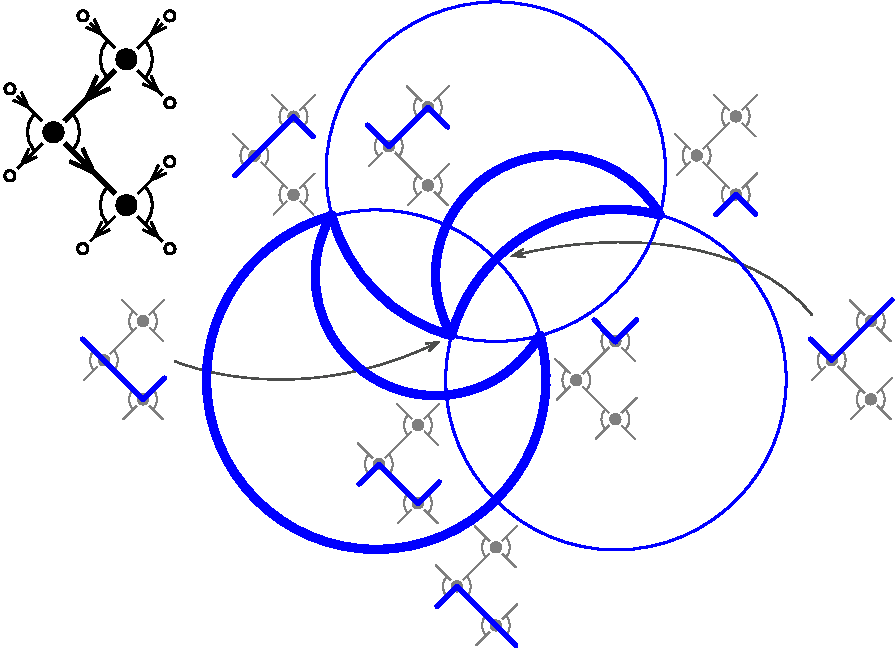
\includegraphics[scale=.6]{fan}}
	\caption{The shards corresponding to the facets of the type cone. Is there a geometric meaning?}
	\label{fig:fanShards}
\end{figure}

%%%%%%%%%%%

\subsection{Graphical nested complexes and graph associahedra}

Graph associahedra were defined by M.~Carr and S.~Devadoss~\cite{CarrDevadoss} in connection to C.~De Concini and C.~Procesi's wonderful arrangements~\cite{DeConciniProcesi}.
For a given graph~$\graphG$, the $\graphG$-associahedron~$\Asso[\graphG]$ is a simple polytope whose combinatorial structure encodes the connected subgraphs of~$\graphG$ and their nested structure.
More precisely, the $\graphG$-associahedron is a polytopal realization of the nested complex of~$\graphG$, defined as the simplicial complex of all collections of tubes (connected induced subgraphs) of~$\graphG$ which are pairwise compatible (either nested, or disjoint and non-adjacent).
As illustrated in~\cref{fig:specialGraphAssociahedra}, the graph associahedra of certain special families of graphs coincide with well-known families of polytopes: complete graph associahedra are permutahedra, path associahedra are classical associahedra, cycle associahedra are cyclohedra, and star associahedra are stellohedra.
The graph associahedra were extended to the \defn{nestohedra}, which are simple polytopes realizing the nested complex of arbitrary building sets~\cite{Postnikov, FeichtnerSturmfels}.
Graph associahedra and nestohedra have been geometrically realized in different ways: by successive truncations of faces of the standard simplex~\cite{CarrDevadoss}, as Minkowski sums of faces of the standard simplex~\cite{Postnikov, FeichtnerSturmfels}, or from their normal fans by exhibiting explicit inequality descriptions~\cite{Devadoss, Zelevinsky}.
For a given graph~$\graphG$, the resulting polytopes all have the same normal fan, called nested fan of~$\graphG$: its rays are the characteristic vectors of the tubes, and its cones are generated by characteristic vectors of compatible tubes.
In this section, we describe the type cone of the nested fan of any graph~$\graphG$.

\begin{figure}[t]
	\capstart
	\centerline{
		\begin{tabular}{c@{\;}c@{\;}c@{\;}c}
    		permutahedron &
    		associahedron &
    		cyclohedron &
    		stellohedron \\
    		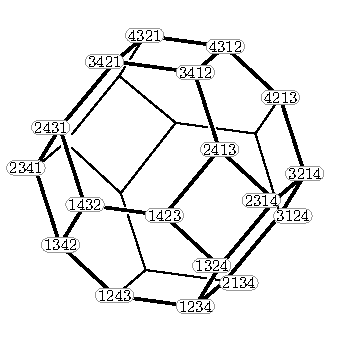
\includegraphics[scale=.6]{permutahedron} &
    		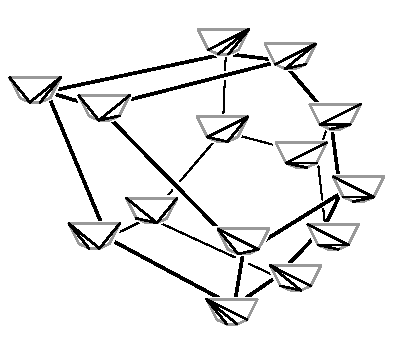
\includegraphics[scale=.6]{associahedron} &
    		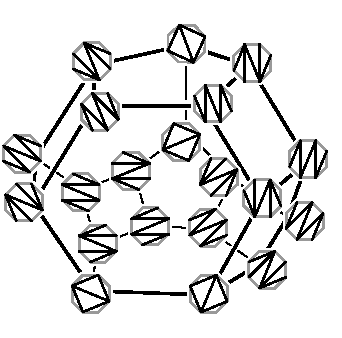
\includegraphics[scale=.6]{cyclohedron} &
    		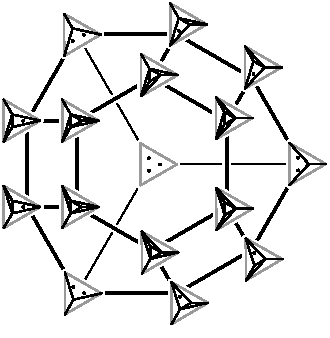
\includegraphics[scale=.6]{stellohedron} \\
    		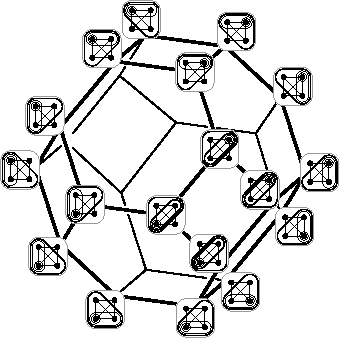
\includegraphics[scale=.6]{permutahedronTubings} &
    		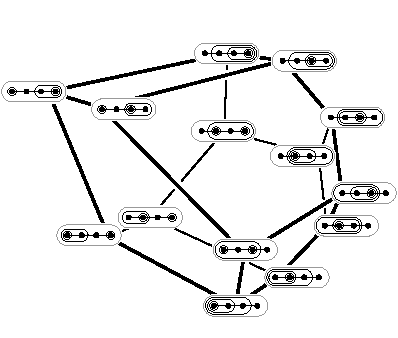
\includegraphics[scale=.6]{associahedronTubings} &
    		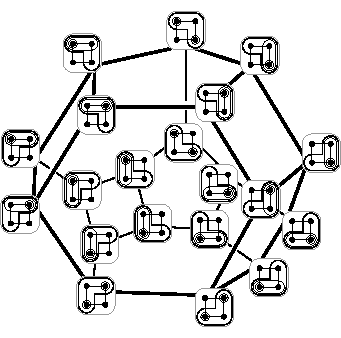
\includegraphics[scale=.6]{cyclohedronTubings} &
    		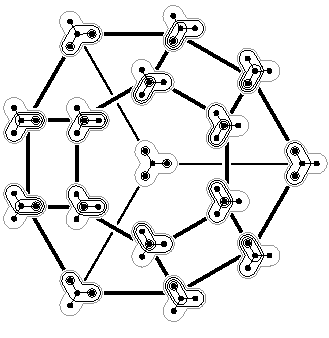
\includegraphics[scale=.6]{stellohedronTubings} \\[.1cm]
    		complete graph &
    		path &
    		cycle &
    		star
		\end{tabular}
	}
	\caption{Some classical families of polytopes as graph associahedra. Illustration from~\cite{MannevillePilaud-compatibilityFans}.}
	\label{fig:specialGraphAssociahedra}
\end{figure}

\subsubsection{Nested complex and nested fan of a graph}

We present the definitions and properties of the nested complex of a graph, following ideas from~\cite{CarrDevadoss, Postnikov, FeichtnerSturmfels, Zelevinsky}.

\para{Nested complex}
%
Let~$\graphG$ be a graph with vertex set~$\ground$.
Let~$\connectedComponents(\graphG)$ denote the set of connected components of~$\graphG$ and define~$n \eqdef |\ground|-|\connectedComponents(\graphG)|$.
A \defn{tube} of~$\graphG$ is a connected induced subgraph of~$\graphG$.
The set of tubes of~$\graphG$ is denoted by~$\tubes(\graphG)$.
The inclusion maximal tubes of~$\graphG$ are its connected components~$\connectedComponents(\graphG)$.
The tubes which are neither empty nor maximal are called \defn{proper}.
Two tubes~$\tube, \tube'$ of~$\graphG$ are \defn{compatible} if they are either nested (\ie $\tube \subseteq \tube'$ or~$\tube' \subseteq \tube$), or disjoint and non-adjacent (\ie $\tube \cup \tube'$ is not a tube of~$\graphG$).
A \defn{tubing} on~$\graphG$ is a set~$\tubing$ of pairwise compatible proper tubes of~$\graphG$.
The \defn{nested complex} of~$\graphG$ is the simplicial complex~$\nestedComplex(\graphG)$ of all tubings on~$\graphG$.

\para{Nested fan and graph associahedron}
%
Let~$(\b{e}_v)_{v \in \ground}$ be the canonical basis of~$\R^\ground$.
We consider the hyperplane~${\HH \eqdef \bigset{\b{x} \in \R^\ground}{\sum_{w \in W} x_w = 0 \text{ for all } W \in \connectedComponents(\graphG)}}$ and let~$\pi : \R^\ground \to \HH$ denote the orthogonal projection on~$\HH$.
The \defn{$\b{g}$-vector} of a tube~$\tube$ of~$\graphG$ is the projection~$\gvector{\tube} \eqdef \pi \big( \sum_{v \in \tube} \b{e}_v \big)$ of the characteristic vector of~$\tube$.
Note that by definition,~$\gvector{\graphG} = 0$.
We also define~$\gvectors{\tubing} \eqdef \set{\gvector{\tube}}{\tube \in \tubing}$ for a tubing~$\tubing$ on~$\graphG$.
These vectors support a complete simplicial fan realization of the nested complex.
Examples are illustrated in \cref{fig:nestedFans}.

\begin{figure}[h]
	\capstart
	\centerline{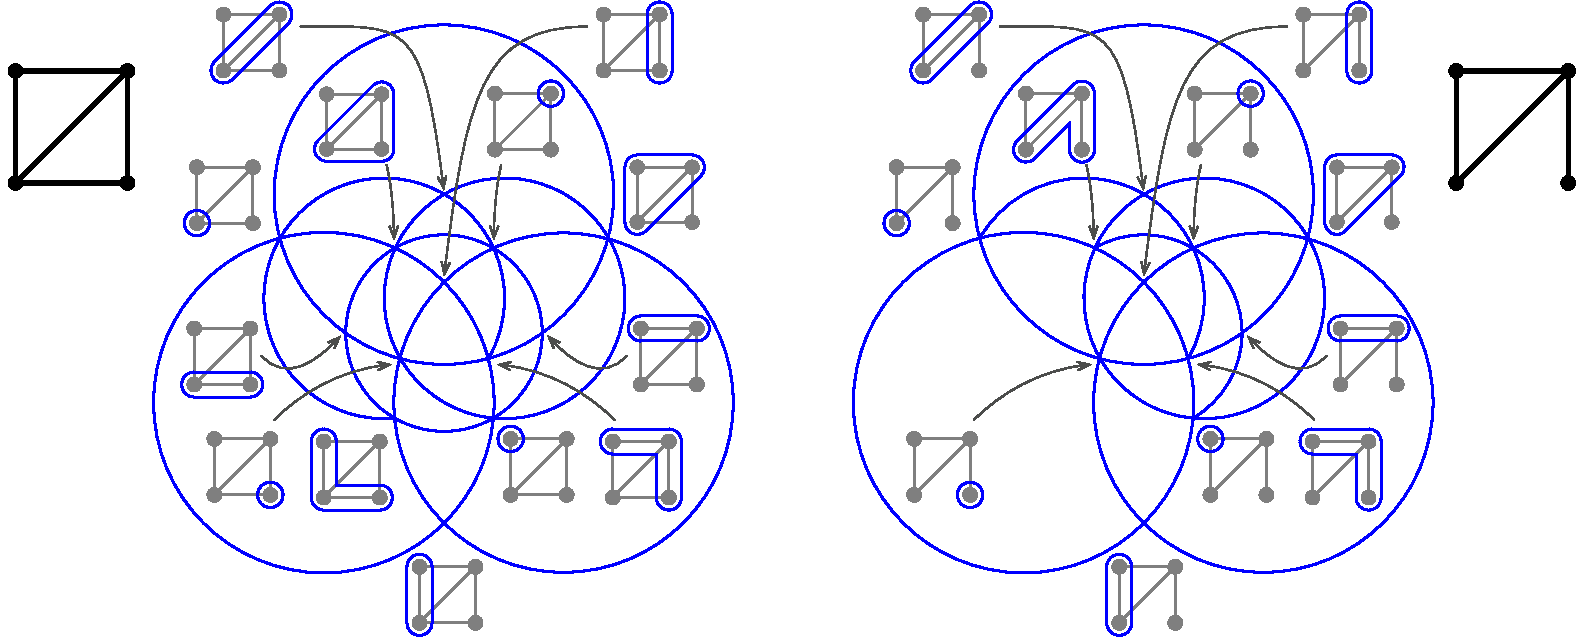
\includegraphics[scale=.55]{nestedFans}}
	\caption{Two nested fans. As the fans are $3$-dimensional, we intersect them with the sphere and stereographically project them from the direction~$(-1,-1,-1)$.}
	\label{fig:nestedFans}
\end{figure}

\begin{theorem}[\cite{CarrDevadoss, Postnikov, FeichtnerSturmfels, Zelevinsky}]
For any graph~$\graphG$, the set of cones
\[
\gvectorFan[\graphG] \eqdef \set{\R_{\ge 0} \, \gvectors{\tubing}}{\tubing \text{ tubing on } \graphG}
\]
is a complete simplicial fan of~$\HH$, called \defn{nested fan} of~$\graphG$, which realizes the nested complex~$\nestedComplex(\graphG)$.
\end{theorem}

It is proved in~\cite{CarrDevadoss, Devadoss, Postnikov, FeichtnerSturmfels, Zelevinsky} that the nested fan comes from a polytope.
For any subset~$U \subseteq \ground$, denote by~$\triangle_U \eqdef \conv\set{\b{e}_u}{u \in U}$ the face of the standard simplex~$\triangle_\ground$ corresponding to~$U$.

\begin{theorem}[\cite{CarrDevadoss, Devadoss, Postnikov, FeichtnerSturmfels, Zelevinsky}]
For any graph~$\graphG$, the nested fan~$\gvectorFan[\graphG]$ is the normal fan of the graph associahedron~$\Asso[\graphG]$, defined as the Minkowski sum~$\sum_{\tube \in \tubes(\graphG)} \triangle_{\tube}$ of the faces of the standard simplex corresponding to all tubes of~$\graphG$.
\end{theorem}

\para{Flips in the nested fan}
%
The following statement follows from~\cite{MannevillePilaud-compatibilityFans, Zelevinsky}.

\begin{proposition}
\label{prop:exchangeablePairsGA}
Let~$\tube, \tube'$ be two tubes of~$\graphG$. Then
\begin{enumerate}[(i)]
\item The tubes~$\tube$ and~$\tube'$ are exchangeable if and only if $\tube'$ has a unique neighbor~$v$ in~$\tube \ssm \tube'$ and $\tube$ has a unique neighbor~$v'$ in~$\tube' \ssm \tube$.
\item For any maximal tubings~$\tubing, \tubing$ on~$\graphG$ with $\tubing \ssm \{\tube\} = \tubing' \ssm \{\tube'\}$, both~$\tubing \cup \connectedComponents(\graphG)$ and~$\tubing' \cup \connectedComponents(\graphG)$ contain the tube~$\tube \cup \tube'$ and the connected components of~$\tube \cap \tube'$.
\item The linear dependence between the $\b{g}$-vectors of~$\tubing \cup \tubing'$ is given by
\[
\gvector{\tube} + \gvector{\tube'} = \gvector{\tube \cup \tube'} + \sum_{\tube[s] \in \connectedComponents(\tube \cap \tube')} \gvector{\tube[s]}.
\]
In other words, the nested fan of~$\graphG$ has the unique exchange relation property.
\item The $\b{c}$-vector orthogonal to all $\b{g}$-vectors~$\gvector{\tube[s]}$ for~$\tube[s] \in \tubing \cap \tubing'$ is~$\b{e}_v - \b{e}_{v'}$.
\end{enumerate}
\end{proposition}

\begin{proof}
Points~(i) and~(ii) was proved in~\cite{MannevillePilaud-compatibilityFans}. Point~(iii) follows from the fact that
\[
\sum_{v \in \tube} \b{e}_v + \sum_{v \in \tube'} \b{e}_v = \sum_{v \in \tube \cup \tube'} \b{e}_v + \sum_{v \in \tube \cap \tube'} \b{e}_v = \sum_{v \in \tube \cup \tube'} \b{e}_v + \sum_{\substack{\tube[s] \in \connectedComponents(\tube \cap \tube') \\ v \in \tube[s]}} \b{e}_v.
\]
Finally for~(iv), any tube~$\tube[s] \in \tubing \cap \tubing'$ that contains~$v$ or~$v'$ actually contains both (to be compatible with~$\tube$ and~$\tube'$). Therefore, $\gvector{\tube[s]}$ is orthogonal to~$\b{e}_v - \b{e}_{v'}$ for any tube~$\tube[s] \in \tubing \cap \tubing'$.
\end{proof}

We are now ready to describe the type cone of the nested fan~$\gvectorFan[\graphG]$.
We first treat the case when~$G$ is a path so that the $\graphG$-associahedron is a classical associahedron.
We show that the type cone is then simplicial which gives another proof of \cref{thm:simplicialTypeConeAsso} and \cref{coro:descriptionAllAsso}.

\subsubsection{Simplicial type cones for path associahedra}

We start with the case of the path on~$n+1$ vertices.
Recall that the tubes of the path are the intervals of~$[n+1]$ and that two intervals~$[i,j]$ and~$[i',j']$ of~$[n+1]$ are exchangeable if either~${i < i' \le j+1 < j'+1}$ or~${i' < i \le j'+1 < j+1}$.

\begin{proposition}
\label{prop:extremalExchangeablePairsA}
%The extremal exchangeable pairs for the nested fan of the path are precisely the pairs of intervals~$\{[i,j], [i+1,j+1]\}$ for~$1 \le i \le j \le n-1$.
Two intervals~$[i,j]$ and~$[i',j']$ of~$[n+1]$ form an extremal exchangeable pair for the nested fan of the path if and only if~$i = i'+1$ and~$j = j'+1$, or the opposite.
\end{proposition}

\begin{proof}
Let~$(\b{f}_{[i,j]})_{1 \le i \le j \le n}$ be the canonical basis of~$\R^{\binom{n+1}{2}}$.
Consider two exchangeable tubes~$[i,j]$ and~$[i',j']$ with~${i < i' \le j+1 < j'+1}$.
By \cref{prop:exchangeablePairsGA}\,(iii), the linear dependence between the corresponding $\b{g}$-vectors is given by
\[
\gvector{[i,j]} + \gvector{[i',j']} = \gvector{[i,j']} + \gvector{[i',j]}.
\]
Therefore, the outer normal vector of the corresponding inequality of the type cone~$\typeCone(\gvectorFan[\graphG])$ is
\[
\b{n}(i,j,i',j') \eqdef \b{f}_{[i,j]} + \b{f}_{[i',j']} - \b{f}_{[i,j']} - \b{f}_{[i',j]}.
\]
Denoting
\[
\b{m}(k,\ell) \eqdef \b{n}(k,\ell-1,k+1,\ell) = \b{f}_{[k, \ell-1]} + \b{f}_{[k+1, \ell]} - \b{f}_{[k, \ell]} - \b{f}_{[k+1, \ell-1]},
\]
we obtain that
\[
\b{n}(i,j,i',j') = \sum_{\substack{k \in {[i,i'[} \\ \ell \in {]j,j']}}} \b{m}(k,\ell).
\]
Indeed, on the right hand side, the basis vector~$\b{f}_{[k,\ell]}$ appears with a positive sign in~$\b{m}(k,{\ell+1})$ for~$(k,\ell) \in {[i,i'[} \times {[j,j'[}$ and in~$\b{m}(k-1, \ell)$ for~$(k,\ell) \in {]i,i']} \times {]j,j']}$, and with a negative sign in~$\b{m}(k,\ell)$ for~$(k,\ell) \in {[i,i'[} \times {]j,j']}$ and in~$\b{m}(k-1,\ell+1)$ for~$(k,\ell) \in {]i,i']} \times {[j,j'[}$.
Therefore, these contributions all vanish except when~$[k, \ell]$ is one of the tubes~$[i,j]$, $[i',j']$, $[i,j']$ or~$[i',j]$.
%For any~$i \le k < i'$ and~$j < \ell \le j'$, the exchange relation between the tubes~$[k, \ell-1]$ and~$[k+1, \ell]$ is given by
%\begin{equation}
%\label{eq:exch2}
%\tag{$\mathrm{ER}_k^\ell$}
%\gvector{[k, \ell-1]} + \gvector{[k+1, \ell]} = \gvector{[k, \ell]} + \gvector{[k+1, \ell-1]}.
%\end{equation}
%Summing the exchange relations~\eqref{eq:exch2} over all pairs~$(k,\ell) \in {[i,i'[} \times {]j,j']}$, we obtain after simplifications the exchange relation~\eqref{eq:exch1}.
%Indeed, the $\b{g}$-vector of each tube~$[k, \ell]$ appears on the left hand sides of the exchange relations~($\mathrm{ER}_k^{\ell+1}$) for~$(k,\ell) \in {[i,i'[} \times {[j,j'[}$ and ($\mathrm{ER}_{k-1}^\ell$) for~$(k,\ell) \in {]i,i']} \times {]j,j']}$ and on the right hand sides of the exchange relations~($\mathrm{ER}_k^\ell$) for~$(k,\ell) \in {[i,i'[} \times {]j,j']}$ and~($\mathrm{ER}_{k-1}^{\ell+1}$) for~$(k,\ell) \in {]i,i']} \times {[j,j'[}$.
%Therefore, these contributions all vanish except when~$[k, \ell]$ is one of the tubes~$[i,j]$, $[i',j']$, $[i,j']$ or~$[i',j]$.
This shows that any exchange relation is a positive linear combination of the exchange relations corresponding to all pairs of tubes~$[i,j]$ and~$[i',j']$ of~$[n+1]$ such that~$i = i'+1$ and~$j = j'+1$.

We now need to show that all these exchangeable pairs are extremal.
Assume that~$\b{m}(k,\ell)$ can be written as the linear combination
\begin{equation}
\label{eq:linComb}
\b{m}(k,\ell) = \sum \lambda(i,j,i',j') \, \b{n}(i,j,i',j'),
\end{equation}
where~$\lambda(i,j,i',j') \ge 0$ for all exchangeable pairs~$\{[i,j], [i',j']\}$.
Note that~$\sum \lambda(i,j,i',j') \ge 1$ since the coefficient of~$\b{f}_{[k,\ell]}$ in~$\b{m}(k,\ell)$ is~$-1$.
Consider the linear form~$\Phi: \R^N \to \R$ defined by~$\Phi(\b{f}_{[i,j]}) = -(j-i)^2$.
A quick computation shows that
\[
\Phi(\b{n}(i,j,i',j')) = 2(i'-i)(j'-j).
\]
Applying~$\Phi$ to \cref{eq:linComb}, we obtain
\[
1 = \sum \lambda(i,j,i',j')(i'-i)(j'-j).
\]
Since~$\sum \lambda(i,j,i',j') \ge 1$ we obtain that~$\lambda(k,\ell-1,k+1,\ell) = 1$ and~$\lambda(i,j,i',j') = 0$ for all other exchangeable pairs~$\{[i,j], [i',j']\}$.
\end{proof}

\subsubsection{General case}

We now consider an arbitrary graph~$\graphG$ and describe the type cone of its nested fan.
\cref{prop:extremalExchangeablePairsA} extends as follows.
% We denote by~$X \symdif Y$ the symmetric difference of two sets~$X$ and~$Y$.

\begin{proposition}
\label{prop:extremalExchangeablePairsGA}
%A pair~$\{\tube, \tube'\}$ of exchangeable tubes of~$\graphG$ is extremal if and only if~$|\tube \symdif \tube'| = 2$.
Two tubes~$\tube$ and~$\tube'$ of~$\graphG$ form an extremal exchangeable pair for the nested fan of~$\graphG$ if and only if~${\tube \ssm \{v\} = \tube' \ssm \{v'\}}$ for some neighbor~$v$ of~$\tube'$ and some neighbor~$v'$ of~$\tube$.
\end{proposition}

\begin{proof}
Consider an exchangeable pair~$\{\tube, \tube'\}$ of tubes of~$\graphG$ and let~$p = |\tube \cup \tube'|$.
By \cref{prop:exchangeablePairsGA}, $\tube'$ has a unique neighbor~$v$ in~$\tube \ssm \tube'$ and $\tube$ has a unique neighbor~$v'$ in~$\tube' \ssm \tube$.
Therefore, $\tube \ssm \tube'$ and~$\tube' \ssm \tube$ are both connected.
We can thus label the elements of~$\tube \cup \tube'$ by~$\{v_1, \dots, v_p\}$ such that~$\{v_i, \dots, v_j\}$ induces a tube~$\tube_{k,\ell}$ of~$\graphG$ for any~$1 \le k \le \ell \le p$. 
The map~$[k,\ell] \mapsto \tube_{k,\ell}$ is thus an injection from the tubes of the path~$\graphG[P]_p$ to that of~$\graphG$ that fulfills
\begin{itemize}
\item $\tube_{k,\ell-1} \ssm \{v_k\} = \tube_{k+1,\ell} \ssm \{v_\ell\}$ for any~$1 \le k \le \ell \le p$, and
\item $\gvector{\tube_{k,\ell}} = M\gvector{[k,\ell]}$ for any~$1 \le k \le \ell \le p$, where~$M$ is the matrix sending~$\b{e}_m$ to~$\b{e}_{v_m}$.
\end{itemize}
Therefore, this map transports the linear combinations of \cref{prop:extremalExchangeablePairsA}.
We conclude that the exchange relation corresponding to the exchangeable pair~$\{\tube, \tube'\}$ is a positive linear combination of the exchange relations corresponding to the pairs~$\{\tube_{k,\ell-1}, \tube_{k+1,\ell}\}$ for all~${(k,\ell) \in {[1, p-|\tube'|+1[} \times {]|\tube|, p]}}$.

We now need to show that all these pairs are extremal.
\vincent{TODO}
\end{proof}

The following statement reformulates \cref{prop:extremalExchangeablePairsGA}.

\begin{corollary}
\label{coro:extremalExchangeablePairsGA}
The extremal exchangeable pairs for the nested fan of~$\graphG$ are equivalently
\begin{enumerate}[(i)]
\item the pairs of tubes~$\tube[r] \cup \{v\}$ and~$\tube[r] \cup \{v'\}$ for any tube~$\tube[r] \in \tubes(\graphG)$ and distinct neighbors~$v,v'$ of~$\tube[r]$,
\item the pairs of tubes~$\tube[s] \ssm \{v'\}$ and~$\tube[s] \ssm \{v\}$ for any tube~$\tube[s] \in \tubes(\graphG)$ and distinct non-disconnecting vertices~$v,v'$ of~$\tube[s]$,
\end{enumerate}
\end{corollary}

We derive from \cref{prop:extremalExchangeablePairsGA} and \cref{coro:extremalExchangeablePairsGA} all polytopal realizations of the nested fan, which we can explicitly express using one of the following two equivalent conditions.

%\begin{corollary}
%Consider a graph~$\graphG$ on~$\ground$ with tubes~$\tubes(\graphG)$ and a height vector~$\b{h} \in \R^{\tubes(\graphG)}$ such that~$\b{h}_{\graphG} = 0$ and
%\[
%\b{h}_{\tube} + \b{h}_{\tube'} > \b{h}_{\tube \cup \tube'} + \sum_{\tube[s] \in \connectedComponents(\tube \cap \tube')} \b{h}_{\tube[s]}
%\]
%for any pair of tubes~$\{\tube, \tube'\}$ of~$\graphG$ with~$\tube \ssm \{v\} = \tube' \ssm \{v'\}$ where~$v$ is a neighbor of~$\tube'$ and~$v'$ is a neighbor of~$\tube$.
%Then the nested fan~$\gvectorFan[\graphG]$ is the normal fan of the graph associahedron
%\[
%\set{\b{x} \in \R^\ground}{\dotprod{\gvector{\tube}}{\b{x}} \le \b{h}_{\tube} \text{ for any tube } \tube \in \tubes(\graphG)}.
%\]
%\end{corollary}

\begin{corollary}
Consider a graph~$\graphG$ on~$\ground$ with tubes~$\tubes(\graphG)$ and a height vector~$\b{h} \in \R^{\tubes(\graphG)}$ such that~$\b{h}_{\varnothing} = \b{h}_{\graphG} = 0$ and satisfying one of the two following equivalent conditions:
\begin{enumerate}[(i)]
\item $\b{h}_{\tube[r] \cup \{v\}} + \b{h}_{\tube[r] \cup \{v'\}} > \b{h}_{\tube[r] \cup \{v, v'\}} + \b{h}_{\tube[r]}$ for any tube~$\tube[r] \in \tubes(\graphG)$ and distinct neighbors~$v,v'$ of~$\tube[r]$,
\item $\b{h}_{\tube[s] \ssm \{v'\}} + \b{h}_{\tube[s] \ssm \{v\}} > \b{h}_{\tube[s]} + \b{h}_{\tube[s] \ssm \{v, v'\}}$ for any tube~$\tube[s] \in \tubes(\graphG)$ and distinct non-disconnecting vertices~$v,v'$ of~$\tube[s]$.
\end{enumerate}
Then the nested fan~$\gvectorFan[\graphG]$ is the normal fan of the graph associahedron
\[
\set{\b{x} \in \R^\ground}{\dotprod{\gvector{\tube}}{\b{x}} \le \b{h}_{\tube} \text{ for any tube } \tube \in \tubes(\graphG)}.
\]
\end{corollary}

We also obtain from \cref{prop:extremalExchangeablePairsGA} the following surprising property.

\begin{corollary}
Any $\b{c}$-vector supports at least one extremal exchangeable pair.
\end{corollary}

\begin{proof}
Consider a $\b{c}$-vector~$\b{e}_v - \b{e}_{v'}$ for two distinct vertices~$v, v'$ in a common connected component of~$\graphG$. Let~$\tube[r]$ be a path from~$v$ to~$v'$ in~$\graphG$ and let~$\tube \eqdef \tube[r] \cup \{v\}$ and~$\tube' \eqdef \tube[r] \cup \{v'\}$. Then $\{\tube, \tube'\}$ is an extremal exchangeable pair with $\b{c}$-vector~$\b{e}_v - \b{e}_{v'}$.
\end{proof}

We derive from~\cref{coro:extremalExchangeablePairsGA} the number of extremal exchangeable pairs of the nested fan.
For a tube~$\tube$ of~$\graphG$, we denote by~$\neighbors(\tube)$ the number of neighbors of~$\tube$ and by~$\nonDisconnecting(\tube)$ the number of non-disconnecting vertices of~$\tube$.
In other words, it $\neighbors(\tube)$ (resp.~$\nonDisconnecting(\tube)$) is the number of tubes covering~$\tube$ (resp.~covered by~$\tube$) in the inclusion poset of all tubes of~$\graphG$.

\begin{corollary}
\label{coro:numberExtremalExchangeablePairsGA}
The nested fan~$\gvectorFan[\graphG]$ has~$\!\!\!\! \sum\limits_{\tube[r] \in \tubes(\graphG)} \!\! \binom{\neighbors(\tube[r])}{2} = \!\!\!\! \sum\limits_{\tube[s] \in \tubes(\graphG)} \!\! \binom{\nonDisconnecting(\tube[s])}{2}$ extremal exchangeable pairs.
\end{corollary}

%\begin{proof}
%By \cref{prop:extremalExchangeablePairsGA}, extremal exchangeable pairs are in bijection with quadruples~$(\tube[r], \tube[t], \tube[t'], \tube[s])$ of tubes of~$\graphG$ where~$\tube[t]$ and~$\tube[t']$ are distinct tubes covering~$\tube[r]$ and covered by~$\tube[s]$ in the inclusion poset of all tubes of~$\graphG$.
%The result immediately follows.
%\end{proof}

The formula of \cref{coro:numberExtremalExchangeablePairsGA} can be made more explicit for specific families of graph associahedra discussed in the introduction and illustrated in \cref{fig:specialGraphAssociahedra}.

\begin{proposition}
The number of extreme exchangeable pairs of the nested fan~$\gvectorFan[\graphG]$ is:
\begin{itemize}
\item $2^{n-2}\binom{n}{2}$ for the permutahedron (complete graph associahedron),
\item $\binom{n}{2}$ for the associahedron (path associahedron),
\item $3\binom{n}{2} - n$ for the cyclohedron (cycle associahedron),
\item $n-1+2^{n-3}\binom{n-1}{2}$ for the stellohedron (star associahedron).
\end{itemize}
\end{proposition}

\begin{proof}
For the permutahedron, choose any two vertices~$v,v'$, and complete them into a tube by selecting any subset of the~$n-2$ remaining vertices.
For the associahedron, choose any two vertices~$v,v'$, and complete them into a tube by taking the path between them.
For the cyclohedron, choose the two vertices~$v,v'$, and complete them into a tube by taking either all the cycle, or one of the two paths between~$v$ and~$v'$ (this gives three options in general, but only two when~$v,v'$ are neighbors).
For the stellohedron, choose either~$v$ as the center of the star and~$v'$ as one of the $n-1$ leaves, or $v$~and~$v'$ as leaves of the star and complete them into a tube by taking the center and any subset of the $n-3$ remaining leaves.
\end{proof}

%\begin{example}
%The formula of \cref{coro:numberExtremalExchangeablePairsGA} can be made more explicit for specific families of graph associahedra:
%\begin{itemize}
%\item the permutahedron (complete graph associahedron) has~$2^{n-2}\binom{n}{2}$ extreme exchangeable pairs (choose the two vertices~$v,v'$, and complete them into a tube by selecting any subset of the~$n-2$ remaining vertices),
%\item the associahedron (path associahedron) has~$\binom{n}{2}$ extreme exchangeable pairs (choose the two vertices~$v,v'$, and complete them into a tube by taking the path between them),
%\item the cyclohedron (cycle associahedron) has~$3\binom{n}{2} - n$ extreme exchangeable pairs (choose the two vertices~$v,v'$, and complete them into a tube by taking either all the cycle, or one of the two paths between~$v$ and~$v'$; this gives three options in general, but only two when~$v,v'$ are neighbors),
%\item the stellohedron (star associahedron) has $n-1+2^{n-3}\binom{n-1}{2}$ extreme exchangeable pairs (choose either~$v$ as the center of the star and~$v'$ as one of the $n-1$ leaves, or $v$~and~$v'$ as leaves of the star and complete them into a tube by taking the center and any subset of the $n-3$ remaining leaves).
%\end{itemize}
%\end{example}

To conclude on graph associahedra, we characterize the graphs~$\graphG$ whose nested fan has a simplicial type cone.

\begin{proposition}
The type cone~$\typeCone(\gvectorFan[\graphG])$ is simplicial if and only if~$\graphG$ is a path.
\end{proposition}

\begin{proof}
Note that any tube~$\tube$ with~$|\tube| \ge 2$ has two non-disconnecting vertices when it is a path, and at least three non-disconnecting vertices otherwise (the leaves of an arbitrary spanning tree of~$\tube$).
Therefore, each tube of~$\tubes(\graphG)$ which is not a singleton contributes to at least one extremal exchangeable pairs.
We conclude that the number of extremal exchangeable pairs is at least:
\[
|\tubes(\graphG)| - |V| = |\tubes(\graphG) \ssm \{\varnothing, \graphG\}| - (|V|-1) = N - n,
\]
with equality if and only if all tubes of~$\graphG$ are paths, \ie if and only if~$\graphG$ is a path.
\end{proof}


%%%%%%%%%%%%%%%%%%%%%%%%%%%%%%%%%%%%%%%

\section{Relations for~$\b{g}$-vectors in finite type cluster algebras via~$2$-Calabi--Yau triangulated categories}

In~\cite{Auslander1984}, M.~Auslander showed that the relations in the Grothendieck group of an Artin algebra are generated by the ones given by almost-split sequences precisely when the algebra is of finite representation type.  Inspired by this result, we will show that a similar statement holds (Theorem~\ref{theo::relations-g-vecteurs}) for the~$\b g$-vectors (or indices) of objects in a~$2$-Calabi--Yau triangulated category. 

\subsection{Setting}\label{sect::setting}
Let~$\field$ be a field.  Let~$\cat$ be a~$\field$-linear triangulated category with suspension functor~$\susp$.  We fix a collection~$\ind(\cat)$ of representatives of isomorphism classes of indecomposable objects of~$\cat$. We will assume the following:
\begin{itemize}
 \item $\cat$ is essentially small (in particular,~$\ind(\cat)$ is a set);
 \item $\cat$ is~$\Hom{}$-finite: for each pair of objects~$X$ and~$Y$, the~$\field$-vector space~$\cat(X,Y)$ is finite-dimensional;
 \item $\cat$ is Krull--Schmidt: the endomorphism algebra of any indecomposable object is local;
 \item $\cat$ is~$2$-Calabi--Yau: for each pair of objects~$X$ and~$Y$, there is an isomorphism of bifunctors
 \[
  \cat(X,\susp Y) \to D\cat(Y,\susp X)
 \]
 where~$D=\Hom{\field}(-,\field)$ is the usual duality of vector spaces;
 \item $\cat$ contains a basic cluster-tilting object~$T=\bigoplus_{i=1}^n T_i$:
 \[
  \textrm{for any object~$X$,} \quad \cat(T, \susp X) = 0 \quad \textrm{if and only if} \quad X\in \add(T),
 \]
 where~$\add(T)$ is the smallest additive full subcategory of~$\cat$ containing the~$T_i$'s and closed under isomorphisms.
\end{itemize}

%%%%%%%%%%%

\subsection{Statement of the theorem}
We need to introduce some notations before stating the main result of this section.  Let~$\Lambda:= \End{\cat}(T)$, and let~$F$ be the functor
\[
 F=\cat(T,-):\cat \xrightarrow{} \MOD \Lambda.
\]

\begin{proposition}[\cite{BuanMarshReiten, KellerReiten}]\label{prop::functor-F}

The functor~$F$ induces an equivalence of~$\field$-linear categories
 \[
  F:\cat/(\susp T) \xrightarrow{} \MOD \Lambda,
 \]
 where~$(\susp T)$ is the ideal of morphisms factoring through an object of~$\add(\susp T)$ and~$\MOD \Lambda$ is the category of finite-dimensional right~$\Lambda$-modules.  This equivalence induces further equivalences between~$\add(T)$ and the category of projective modules, and between~$\add(\susp^2 T)$ and that of injective modules.
\end{proposition}

For categories with a cluster-tilting objects, the~$2$-Calabi--Yau condition implies other duality results which we shall need.

\begin{proposition}[\cite{Palu}]
 For any pair of objects~$X$ and~$Y$ in~$\cat$, there is an isomorphism of bifunctors
 \[
  (\susp T)\cat(X, \susp Y) \xrightarrow{\cong} \cat(Y, \susp X)/(\susp T),
 \]
 where~$(\susp T)\cat(X, \susp Y)$ is the space of morphisms from~$X$ to~$Y$ factoring through~$(\susp T)$.
\end{proposition}

\begin{remark}
 Although the field~$\field$ is assumed to be algebraically closed in~\cite{Palu}, this assumption is not needed in the proof, and the result is valid over any field.
\end{remark}

Finally, we need the existence of almost-split triangles in~$\cat$.  Recall that a triangle
\[
 X\xrightarrow{f} Y \xrightarrow{g} Z \xrightarrow{h} \susp X
\]
in~$\cat$ is \defn{almost-split} if~$X$ and~$Z$ are indecomposable,~$h$ is non-zero, and any non-section~$X\to X'$ factors through~$f$  (or equivalently, any non-retraction~$Z'\to Z$ factors through~$g$).  We say that a triangulated category \defn{has almost-split triangles} if there is an almost-split triangle as above for any indecomposable object~$X$. 

\begin{proposition}[Proposition I.2.3 of~\cite{ReitenVandenbergh}]
 Any triangulated category admitting a Serre functor has almost-split triangles.  In particular, any~$2$-Calabi--Yau triangulated category has almost-split triangles.
\end{proposition}

\begin{definition}\label{defi::grothendieck-group}
 \begin{enumerate}
  \item Let~$\Ksp(\cat)$ be the \defn{split Grothendieck group} of~$\cat$, that is, the free abelian group generated by symbols~$[X]$, where~$[X]$ denotes the isomorphism class of~$X$ in~$\cat$, modulo the following relations: for any objects~$Y$ and~$Z$, we let~$[Y\oplus Z] = [Y] + [Z]$. 
  
  \item Let~$\Kg(\cat)$ be the quotient of~$\Ksp(\cat)$ by the relations~$[X]+[Z]-[Y]$ for all triangles
  \[
   X\xrightarrow{} Y \xrightarrow{} Z \xrightarrow{h} \susp X
  \]
  with~$h\in (\susp T)$.  Denote by~$\b g:\Ksp(\cat) \to \Kg(\cat)$ the canonical projection.

 \end{enumerate}

 
\end{definition}
In particular,~$\Ksp(\cat)$ is isomorphic to a free abelian group over the set~$\ind(\cat)$.  The choice of the notation for~$\Kg(\cat)$ is motivated by Section~\ref{sect::applications-g-vectors}, where we study relations between~$\b g$-vectors.

\begin{definition}\label{defi::bilinear form}
 For any two objects~$X$ and~$Y$ of~$\cat$, define
 \[
  \langle X, Y \rangle := \dim_{\field} \Hom{\Lambda}(FX,FY).
 \]
 This defines a bilinear form
 \[
  \langle -,-\rangle : \Ksp(\cat) \times \Ksp(\cat) \xrightarrow{} \Z.
 \]
\end{definition}

\begin{notation}\label{notation::ell_X}
\begin{enumerate}
 \item For any indecomposable object~$X$ of~$\cat$, let
 \[
  X \to E \to \susp^{-1} X \to \susp X
 \]
 be an almost split triangle (unique up to isomorphism).  We let
 \[
  \ell_X := [X] + [\susp^{-1} X]  - [E] \in \Ksp(\cat).
 \]
 
 \item For any indecomposable object~$Y$ of~$\cat$, let
 \[
  \susp Y \to E' \to  Y \to \susp^2 Y
 \]
 be an almost split triangle (unique up to isomorphism).  We let
 \[
  r_Y := [Y] + [\susp Y]  - [E'] \in \Ksp(\cat).
 \]
\end{enumerate}
\end{notation}


We can finally state the main theorem of this section, which is an analogue of the main result of~\cite{Auslander1984}.

\begin{theorem}\label{theo::relations-g-vecteurs}
 Let~$\cat$ be a category satisying the hypotheses of Section \ref{sect::setting}.  Then~$\cat$ has only finitely many isomorphism classes of indecomposable objects if and only if the set~\[L:=\big\{\ell_X \ | \ X\in \ind(\cat)\setminus \add(\susp T) \big\}\] generates the kernel of~$\b g:\Ksp(\cat) \to \Kg(\cat)$. 
 In this case, the set~$L$ is a basis of the kernel of~$\b g$, and for any $x\in \ker(\b g)$, we have that
 \[
  x= \sum_{A\in \ind(\cat) \setminus \add(\susp T)} \frac{\langle x, A \rangle}{\langle \ell_A, A \rangle} \ell_A.
 \]
\end{theorem}

\begin{corollary}
 Assume that~$\ind(\cat)$ is finite.  Let~$X\xrightarrow{} E \xrightarrow{} Y \xrightarrow{h} \susp X$ be a triangle with~$h\in (\susp T)$.  Then the element~$x=[X]+[Y]-[E]$ of the kernel of~$\b g$ is a non-negative linear combination of the~$\ell_A$, with~$A\in \ind(\cat)\setminus \add(\susp T)$.
\end{corollary}
\begin{proof}
 We know that~$x=\sum_{A\in \ind(\cat)\setminus \add(\susp T)} \frac{\langle x, [A] \rangle}{\langle \ell_A, [A] \rangle} \ell_A$; since~$\langle \ell_A, [A] \rangle$ is positive by Lemma~\ref{lemm::bilinear-form}, we only need to show that each~$\langle x, [A] \rangle$ is non-negative. 
 The functor~$F=\cat(T,-)$ induces an exact sequence
 \[
  FX \to FE \to FY \to 0,
 \]
 which in turn induces an exact sequence
 \[
  0\to \Hom{\Lambda}(FY, FA) \to \Hom{\Lambda}(FE, FA) \xrightarrow{f} \Hom{\Lambda}(FX, FA) \to \coker(f) \to 0.
 \]
 Therefore~$\langle x, [A] \rangle = \dim_{\field} \coker(f) \geq 0$.
\end{proof}

%%%%%%%%%%%

\subsection{Proof of Theorem \ref{theo::relations-g-vecteurs}}

Before we can prove Theorem~\ref{theo::relations-g-vecteurs}, we need to recall the following results and definition from \cite{DehyKeller,Palu}.

\begin{proposition}
 Let~$X$ be an object of~$\cat$. Then there exists a triangle
 \[
  T_1^X \to T^0_X \to X \to \susp T_1^X
 \]
 with~$T_1^X$ and~$T_0^X$ in~$\add(T)$.

\end{proposition}

\begin{definition}
 The \defn{index} of an object~$X$ is the element
 \[
  \ind_T(X) := [T_0^X] - [T_1^X] \in \Ksp(\add(T)).
 \]
\end{definition}

The notion of index is very close to the definition of the map~$\b g:\Ksp(\cat)\to \Kg(\cat)$ of Definition~\ref{defi::grothendieck-group}.  The link is given by the following result.

\begin{proposition}[\cite{Palu}]
 Let~$X\xrightarrow{} Y \xrightarrow{} Z \xrightarrow{h} \susp X$ be a triangle.
 Then
 \[
  \ind_T(X) + \ind_T(Z) - \ind_T(Y) = 0
 \]
 if and only if~$h\in (\susp T)$.
\end{proposition}

\begin{corollary}\label{coro::grothendieck-g-vectors}
 There is an isomorphism~$\phi:\Kg(\cat) \to \Ksp(\add(T))$ such that~$\ind_T = \phi\circ \b g$.  In particular,~$\Kg(\cat)$ is a free abelian group generated by the~$[T_i]$.
\end{corollary}

We can now begin the proof of Theorem~\ref{theo::relations-g-vecteurs}

\begin{lemma}\label{lemm::bilinear-form-suspention-T}
 If~$X$ or~$Y$ lie in~$\add(\susp T)$, then~$\langle X, Y \rangle = 0$.
\end{lemma}
\begin{proof}
 This is because~$F\susp T = 0$.
\end{proof}

\begin{lemma}\label{lemm::almost-split}
 Let~$X\xrightarrow{} Y \xrightarrow{} \susp^{-1} X \xrightarrow{h} \susp X$ be an almost-split triangle.  Then~$X\notin \add(\susp T)$ if and only if~$h\in (\susp T)$.
\end{lemma}
\begin{proof}
 If~$X\in \add(\susp T)$, then~$h$ cannot be in~$(\susp T)$, otherwise it would be zero since~$\cat(T, \susp T) =0$.  
 
 Assume now that~$X\notin \add(\susp T)$.  Let~$\field_X$ be the residue field of the algebra~$\End{\cat}(X)$. 
 By definition of an almost-split triangle,~$h$ is in the socle of the right~$\End{\cat}(X)$-module~$\cat(\susp^{-1} X, \susp X)$.  Moreover, this socle is a one-dimensional~$\field_X$-vector space; indeed, the~$2$-Calabi--Yau condition gives an isomorphism
 \[
  \cat(\susp^{-1} X, \susp X) \cong D\cat(X, X).
 \]
 Thus the socle of the right module~$\cat(\susp^{-1} X, \susp X)$ has the same~$\field_X$ dimension as the top of the left module~$\cat(X,X)$.  Since~$X$ is indecomposable,~$\cat(X,X)$ is local, and its top is one-dimensional over~$\field_X$.
 
 Now,~$(\susp T)\cat(\susp^{-1} X, \susp X)$ is a sub-module of~$\cat(\susp^{-1} X, \susp X)$.  Therefore, if~$(\susp T)\cat(\susp^{-1} X, \susp X)$ is non-zero, then it contains the one-dimensional socle of~$\cat(\susp^{-1} X, \susp X)$, and thus contains~$h$.   
 By \cite{Palu},
 \[
  (\susp T)\cat(\susp^{-1} X, \susp X) \cong D\cat(X, X)/(\susp T). 
 \]
The identity morphism of~$X$ is not in~$(\susp T)$, since~$X$ is not in~$\add(\susp T)$.  Thus the right-hand side is non-zero, and so neither is the left-hand side.  By the above, this implies that~$h\in (\susp T)\cat(\susp^{-1} X, \susp X)$, which finishes the proof.
\end{proof}



\begin{lemma}\label{lemm::bilinear-form}
Let~$A$ and~$B$ be two indecomposable objects of~$\cat$. \pg{introduce general notation for redisue field}
\begin{enumerate}
 \item If~$A \notin \add(\susp T)$, then
 \[
  \langle \ell_A, B \rangle = \begin{cases}
                               0 & \textrm{if~$A\ncong B$;} \\
                               \dim_{\field}\field_A & \textrm{if~$A\cong B$.}
                              \end{cases}
 \]
 
 \item If~$B \notin \add(\susp T)$, then
 \[
  \langle A, r_B \rangle = \begin{cases}
                               0 & \textrm{if~$A\ncong B$;} \\
                               \dim_{\field}\field_B & \textrm{if~$A\cong B$.}
                              \end{cases}
 \]
\end{enumerate} 
\end{lemma}
\begin{proof}
 We only prove the first assertion; the second one is proved dually.  Assume that~$A\notin\add(\susp T)$.  Let
 \[
  A \xrightarrow{f} E \xrightarrow{} \susp^{-1} A \xrightarrow{h} \susp A
 \]
 be an almost-split triangle.  By Lemma~\ref{lemm::almost-split}, the morphism~$h$ is in~$(\susp T)$.  Applying the functor~$F=\cat(T,-)$, we get an exact sequence
 \[
  FA\xrightarrow{Ff} FE \xrightarrow{} F\susp^{-1} A \xrightarrow{} 0.
 \]
 Applying now the functors~$\cat(-, B)$ and~$\Hom{\Lambda}(-, FB)$, we get a commutative diagram whose rows are exact sequences and whose vertical maps are surjective by Proposition~\ref{prop::functor-F}.
 \[
  \xymatrix{ & \cat(\susp^{-1} A, B)\ar[r]\ar@{->>}[d] & \cat(E, B)\ar[r]^{f^*}\ar@{->>}[d] & \cat(A,B)\ar[r]\ar@{->>}[d] & \coker(f^*)\ar[r]\ar@{->>}[d] & 0 \\
  0 \ar[r] & \Hom{\Lambda}(F\susp^{-1} A, FB)\ar[r] & \Hom{\Lambda}(FE, FB)\ar[r]^{Ff^*} & \Hom{\Lambda}(FA, FB)\ar[r] & \coker(Ff^*)\ar[r] & 0.
  }
 \]

 If~$B\ncong A$, then the definition of an almost-split triangle implies that~$f^*$ is surjective.  Thus~$\coker(f^*)=0$, so that~$\coker(Ff^*) = 0$, and by additivity of the dimension in exact sequences, we get that~$\langle \ell_A, B \rangle =0$.
 
 If~$B\cong A$, then~$\coker(f^*)$ is isomorphic to the residue field~$\field_A$ of~$\cat(A,A)$.  Since~$A$ is not in~$\add(\susp T)$, the ideal of endomorphisms of~$A$ factoring through an object of~$\add(\susp T)$ is contained in the maximal ideal of~$\cat(A,A)$.  Therefore, the rightmost morphism in the commutative diagram is an isomorphism, so~$\coker(Ff^*)$ is isomorphic to~$\field_A$.
\end{proof}

\begin{lemma}\label{lemm::coefficients}
 Let~$x\in \Ksp(\cat)$, and write~\[x=\sum_{A\in \ind(\cat)} \lambda_A [A].\]  Then for any~$A\in\ind(\cat)\setminus \add(\susp T)$, we have that
 \[
  \lambda_A = \frac{\langle \ell_A, x \rangle}{\langle \ell_A, A \rangle} = \frac{\langle x, r_A \rangle}{\langle A, r_A \rangle}.
 \]
\end{lemma}
\begin{proof}
 Let~$B\in \ind(\cat) \setminus \add(\susp T)$.  Applying Lemma~\ref{lemm::bilinear-form}, we get that
 \[
  \langle \ell_B, x \rangle = \langle \ell_B, \sum_{A\in \ind(\cat)} \lambda_A [A] \rangle = \sum_{A\in \ind{\cat}} \lambda_A \langle \ell_B, [A] \rangle = \lambda_B \langle \ell_B, [B] \rangle.
 \]
 The equality~$\lambda_A = \frac{\langle x, r_A \rangle}{\langle A, r_A \rangle}$ is proved in a similar way.
\end{proof}

\begin{corollary}\label{lemm::test-susp-T}
 Let~$x\in \Ksp(\cat)$.  Then the following are equivalent.
 \begin{enumerate}
  \item $x\in \Ksp(\add(\susp T))$;
  \item $\langle x, [A]\rangle = 0$ for all~$A\in \ind(\cat)$;
  \item $\langle [A], x \rangle = 0$ for all~$A\in \ind(\cat)$.
 \end{enumerate}
\end{corollary}
\begin{proof}
 We will only proof that (1) is equivalent to (2); the proof that (1) is equivalent to (3) is similar.  
 
 Assume that (2) holds.  Then, by Lemma~\ref{lemm::coefficients}, we have that
 \[
  x = \sum_{A\in \ind(\cat)\setminus \add(\susp T)} \frac{\langle \ell_A, x \rangle}{\langle \ell_A, A \rangle}[A] + \sum_{i=1}^n \lambda_{\susp T_i} [\susp T_i] = \sum_{i=1}^n \lambda_{\susp T_i} [\susp T_i].
 \]
 Thus~$x\in \Ksp(\add(\susp T))$, and (1) holds.
 
 Assume now that (1) holds.  Then~$\langle x, [A]\rangle = 0$ for any~$A$ by Lemma~\ref{lemm::bilinear-form-suspention-T}.  Thus (2) holds.
\end{proof}

\begin{proposition}\label{prop::free-set}
 \begin{enumerate}
  \item The set~$\{[\ell_A] \ | \ A\in \ind(\cat) \setminus \add(\susp T) \} \cup \{[\susp T_i] \ | \ i=1, \ldots, n\}$ is free in~$\Ksp(\cat)$.
  \item The set~$\{[r_A] \ | \ A\in \ind(\cat) \setminus \add(\susp T) \} \cup \{[\susp T_i] \ | \ i=1, \ldots, n\}$ is free in~$\Ksp(\cat)$.
 \end{enumerate}
\end{proposition}
\begin{proof}
 We only prove (1); the proof of (2) is similar.  Assume that~
 \[
  x= \sum_{A\in \ind(\cat) \setminus \add(\susp T)} \lambda_A \ell_A + \sum_{i=1}^n \lambda_i [\susp T_i] = 0.
 \]
 Then~$\langle x, [A] \rangle = 0$ for all~$A\in\ind(\cat) \setminus \add(\susp T)$.  But~$\langle x, [A] \rangle = \lambda_A$ by Lemma~\ref{lemm::bilinear-form}.  Thus~
 \[
  x = \sum_{i=1}^n \lambda_i [\susp T_i] = 0.
 \]
 But the~$[\susp T_i]$ are linearly independent in~$\Ksp(\cat)$.  Thus~$\lambda_i = 0$ for all~$i\in \{1, \ldots, n\}$.  This finishes the proof.
\end{proof}

\begin{proposition}
 Assume that~$\ind(\cat)$ is finite.  Then the set~$\{[\ell_A] \ | \ A\in \ind(\cat) \setminus \add(\susp T) \}$ is a basis of the kernel of~$\b g$.  Moreover, for any~$x\in \ker \b g$, we have that
 \[
  x= \sum_{A\in \ind(\cat) \setminus \add(\susp T)} \frac{\langle x, A \rangle}{\langle \ell_A, A \rangle} \ell_A.
 \]
\end{proposition}
\begin{proof}
By Proposition~\ref{prop::free-set}, the set is free.  Let~$x\in \ker \b g$.  Consider the element
\[
 z = x- \sum_{A\in \ind(\cat) \setminus \add(\susp T)} \frac{\langle x, A \rangle}{\langle \ell_A, A \rangle} \ell_A.
\]
Then for any~$B\in \ind{\cat}$, we have that
\[
 \langle  z, [B] \rangle = \Big\langle x- \sum_{A\in \ind(\cat) \setminus \add(\susp T)} \frac{\langle x, A \rangle}{\langle \ell_A, A \rangle} \ell_A, [B] \Big\rangle = \langle x, [B] \rangle - \langle x, [B] \rangle = 0, 
\]
where the second equality is obtained by using Lemma~\ref{lemm::bilinear-form}.  By Lemma~\ref{lemm::test-susp-T}, this implies that~$z\in \Ksp(\add(\susp T))$.  Since~$z\in \ker(\b g)$ and since~$\b g$ is injective on~$\Ksp(\add (\susp T))$ by Corollary~\ref{coro::grothendieck-g-vectors}, we get that~$z=0$.  This finishes the proof.
\end{proof}

\begin{corollary}
 If~$\ind(\cat)$ is finite, then the set~\[\{[\ell_A] \ | \ A\in \ind(\cat) \setminus \add(\susp T) \} \cup \{[\susp T_i] \ | \ i=1, \ldots, n\}\] is a basis of~$\Ksp(\cat)$.
\end{corollary}
\begin{proof}
 By Proposition~\ref{prop::free-set}, the set is free.  It suffices to prove that it generates~$\Ksp(\cat)$.  Let~$x\in \Ksp(\cat)$.  Consider
 \[
  z = x - \sum_{A\in \ind{\cat}} \frac{\langle x, A \rangle}{\langle \ell_A, A\rangle} \ell_A.
 \]
 Then for any~$B\in \ind(\cat)$, we have that~$\langle z, [B] \rangle = 0$.  By Lemma~\ref{lemm::test-susp-T}, this implies that~$z\in \Ksp(\add(\susp T))$, and finishes the proof.
\end{proof}


All that remains is to prove the converse in the statement of Theorem~\ref{theo::relations-g-vecteurs}.

\begin{proposition}
 Assume that the set~$\{[\ell_A] \ | \ A\in \ind(\cat) \setminus \add(\susp T) \}$ is a basis of the kernel of~$\b g$. Then~$\ind(\cat)$ is finite.
\end{proposition}
\begin{proof}
 Let~$x\in \ker \b g$, and write~$x = \sum_{[A]\in \ind(\cat)} \lambda_A[A]$, where the sum has finite support.  For any~$B$ not in the support of the sum, we have that~$\langle x, [B] \rangle = 0$.
 
 Now,~$[T]+[\susp T]$ is in the kernel of~$\b g$, but~$\langle [T] + [\susp T], [B] \rangle = \langle [T], [B] \rangle = 0$ if and only if~$B\in \add(\susp T)$.  Thus~$\ind(\cat)$ has to be finite.
\end{proof}

%%%%%%%%%%%

\subsection{Application to~$\b g$-vectors}\label{sect::applications-g-vectors}

\subsection{Application to~$\b g$-vectors of cluster algebras of finite type}\label{sect::applications-g-vectors}



\begin{theorem}[]\pg{cite???}
 Let~$\cat$ be the cluster category of a valued quiver of Dynkin type~$A,B,C,D,E,F$ or~$G$.  Let~$T$ be a basic cluster-tilting object in~$\cat$, and let~$Q$ be the valued Gabriel quiver of~$\End{\cat}(T)$.  Then there is a bijection
 \[
  \CC: \ind(\cat) \xrightarrow{} \{\textrm{cluster variables in the cluster algebra of~$Q$}\},
 \]
 which has the follwing properties.
 \begin{itemize}
  \item For any~$X,Y\in \ind(\cat)$, $\CC(X)$ and~$\CC(Y)$ are compatible if and only if~$\cat(X, \susp Y) = 0$.
  \item For any~$X\in \ind(\cat)$, the~$\b g$-vector of~$\CC(X)$ is~$\b g([X])$, where we identify~$\Z^n$ and~$\Kg(\cat)$ via the isomorphism sending~$(a_1, \ldots, a_n)$ to~$\sum_{i=1}^n a_i [T_i]$.
  \item For any~$X,Y\in \ind(\cat)$, $\CC(X)$ and~$\CC(Y)$ are exchangeable if and only if~$\dim_{\field_X}\cat(X, \susp Y) = \dim_{\field_Y}\cat(X, \susp Y) = 1$.
 \end{itemize}
\end{theorem}

The cluster category also contains enough information to detect positive mutations.

\begin{proposition}
 Let~$X,Y\in \ind(\cat)$ be such that~$\dim_{\field_X}\cat(X, \susp Y) = \dim_{\field_Y}\cat(X, \susp Y) = 1$.  Let 
 \[
  X\xrightarrow{} E \xrightarrow{} Y \xrightarrow{h} \susp X 
 \]
 be triangle with~$h$ non-zero (this triangle is unique up to isomorphism).  Then~$\CC(Y)$ is obtained by performing a positive mutation on~$\CC(X)$ in some seed if and only if~$h\in (\susp T)$.
 \begin{proof}
  \pg{TO DO, Vincent: definition of positive mutation?}
 \end{proof}
\end{proposition}


%%%%%%%%%%%%%%%%%%%%%%%%%%%%%%%%%%%%%%%
\section{Relations for~$\b{g}$-vectors in brick algebras via extriangulated categories}
\label{sect::extricats}
%%%%
\subsection{Setting}\label{setting::extricat}

\vspace{.4cm}
\noindent {\bf Setting for Section~\ref{sect::prelim on extricats}}
In that section, we let~$\cat$ be an extriangulated category with a fixed full additive \yann{additive contains strictly full + stable under taking summands} subcategory~$\tc$ satisfying the following three properties:
\begin{enumerate}
 \item Every~$T\in\tc$ is projective in~$\cat$;
 \item For each~$T\in\tc$, the morphism~$T\to 0$ is an inflation for the extriangulated structure of~$\cat$;
 \item For each~$X\in\cat$, there is an extriangle~$T_1^X\infl T_0^X \defl X \overset{\delta_X}{\dashrightarrow}$ in~$\cat$ with~$T_0^X, T_1^X$ in~$\tc$.
\end{enumerate}

\noindent {\bf Setting for Section~\ref{sect::Statment extricats}}
In that section, we keep the previous setting, but assume moreover that~$\cat$ is Krull--Schmidt, $\field$-linear, Ext-finite, and has Auslander--Reiten--Serre duality, and that the subcategory~$\tc$ is of the form~$\add T$, where~$T=T_1\oplus\cdots\oplus T_n$ is a basic object.

\begin{remark}
 Examples of categories satisfying the properties above are
 \begin{itemize}
  \item $2$-Calabi--Yau triangulated categories admitting a cluster-tilting object (see Section~\ref{sect::2CYTriangulated});
  \item $2$-Calabi--Yau Frobenius exact categories (see Section~\ref{sect::2CYexact});
  \item for any Artin algebra~$\Lambda$, the category~$K^{[-1,0]}(\proj \Lambda)$ of complexes of finitely generated projective~$\Lambda$-modules concentrated in degrees~$-1$ and~$0$, with morphisms considered up to homotopy (see Section~\ref{sect::Kbproj});
  \item more generally, extriangulated categories~$\cat$ constructed as follows: if~$\tc$ is a rigid subcategory of an extriangulated category~$\ec$, we let~$\cat$ be the full subcategory of~$\ec$ whose objects satisfy condition (3), equipped with the extriangulated structure obtained from that of~$\ec$ by considering those extriangles in~$\ec$ all whose terms belong to~$\cat$ and whose deflation is~$\tc$-epi (see Section~\ref{sect::Rigid}).
 \end{itemize}
\end{remark}

\yann{Rappels sur les categories extriangulees}
%%%%
\subsection{Statement of preliminary results on extriangulated categories}
\label{sect::prelim on extricats}

So as to be able to state the main theorem of Section~\ref{sect::extricats}, we need a few results on extriangulated categories.
However, all proofs are postpone to Section~\ref{sect::proofs extricats}.

We let~$\cat$ be as in Setting~\ref{setting::extricat}.

\begin{notation}
For any object~$T\in\tc$, we fix an extriangle~$T\infl 0 \defl \susp T \dashrightarrow$.
% Extending by additivity, this defines (uniquely up to isomorphism) an object~$\susp T$, for each object~$T\in\tc$.
\end{notation}

\begin{remark}
 As will be proven below [REF], this notation extends to an equivalence of categories from the category~$\tc$ of projective objects in~$\cat$ to the category~$\susp\tc$ of injective objects in~$\cat$.
\end{remark}


\begin{notation}
We let~$\Modt$ denote the category of additive functors from~$\tc$ to Abelian groups, and~$\modt$ its full subcategory of functors that are finitely presented, i.e. cokernels of morphisms between representable functors.
We let~$F:\cat\to\Modt$ be the functor defined on objects by sending~$X\in\cat$ to~$\cat(-,X)|_\tc$.
\end{notation}

\begin{lemma}
For any~$X\in\cat$, the functor~$FX$ is finitely presented.
We thus have a functor
\[
F:\cat\to\modt.
\]
\end{lemma}

Proposition~\ref{prop::KRextricat} below extends similar results from [REF]\yann{ref: BMR, KR ,KZ, IY...} (see also Proposition~\ref{prop::functor-F}) to the setting under consideration. We note that the proof requires minor modifications.

\begin{proposition}\label{prop::KRextricat}
The functor~$F$ induces an equivalence of categories
\[
F: \cat/(\susp\tc) \to \modt
\]
where~$(\susp\tc)$ is the ideal of morphisms factoring through an object of the form~$\susp T$, for some~$T\in\tc$.
% This equivalence induces further equivalences between~$\tc$ and the category of projectives, and between~$\tau\susp\tc$ and that of injectives.
\end{proposition}

\begin{remark}
Because the category~$\cat$ does not have weak kernels in general, the category~$\modt$ might not be abelian.
However, in all our applications, the subcategory~$\tc$ is of the form~$\add(T)$ for some object~$T$.
In that case,~$\modt$ is equivalent to~$\MOD\End{\cat}(T)$ and thus abelian.
\end{remark}

\yann{Applying $X\mapsto\mathbb{E}(-,X)|_{\susp\tc}$ might solve this issue?}

\begin{definition}
We let~$\kzero{\cat}$ denote the Grothendieck group of~$\cat$, that is, the quotient of the free abelian group generated by symbols~$[X]$, for each $X\in\cat$, by the relations~$[X]-[Y]+[Z]$, for each conflation~$X\infl Y\defl Z$ in~$\cat$.
\end{definition}

\begin{remark}
Since~$\tc$ is extension-closed in~$\cat$, it inherits an extriangulated structure.
Because~$\tc$ is made of projective objects in~$\cat$, its extriangulated structure splits and we have~$\kzero{\tc}\cong\Ksp(\tc)$.
\end{remark}


The notion of index from \yann{ref RVdB, DK, P, also studied in ....} generalises to our current setting.

\begin{definition}
For any object~$X\in\cat$, fix some extriangle
\[
T_1^X \infl T_0^X \defl X \overset{\delta_X}{\dashrightarrow}
\]
and define
\[
\ind_\tc X = [T_0^X]-[T_1^X]\in\kzero{\tc}.
\]
\end{definition}

\begin{proposition}
 The assignment~$X\mapsto\ind_\tc X$ is well-defined and induces an isomorphism
\[
\ind_\tc : \kzero{\cat} \overset{\cong}{\longrightarrow} \kzero{\tc}
\]
of abelian groups.
\end{proposition}

\subsection{Statement of the theorem}
\label{sect::Statment extricats}

Let~$\cat$ be as in Setting~\ref{setting::extricat}.

\begin{remark}
Assume moreover that~$\cat$ is $\field$-linear and Ext-finite.
By the preliminary results of Section~\ref{subsection: prelim on extricats}, we can apply~\cite[Proposition 4.2]{IyamaNakaokaPalu} to obtain that~$\modt$ is Hom-finite.
In particular, if $\tc=\add T$, then $\End{\cat}(T)$ is a finite-dimensional~$\field$-algebra.
It thus also follows that Definition~\ref{defi::bilinear form} still makes sense in this more general settup: For any~$X,Y\in\cat$,
\[
\langle X,Y\rangle := \dim_\field \Hom{\tc}(FX,FY) = \dim_\field \cat/(\susp\tc)(X,Y).
\]
\end{remark}

When this makes sense, we make use of Notation~\ref{notation::ell_X}: if
\[
X \infl E \defl Y \dashrightarrow
\]
is an almost-split sequence (see~\cite{IyamaNakaokaPalu} for a definition in this setting), we let
\[
 \ell_X := [X]+[Y]-[E]\in\Ksp(\cat).
\]


\begin{theorem}\label{theorem::extricats}
Assume that~$\cat$ is a~$\field$-linear, Ext-finite, Krull--Schmidt, extriangulated category with Auslander--Reiten--Serre duality.
Assume that~$T$ is a projective object of~$\cat$ such that any~$X\in\cat$ admits an extriangle~$T_1^X\infl T_0^X\defl X\dashrightarrow$ with~$T_0^X, T_1^X\in\add(T)$, and the morphism~$T\to 0$ is an inflation. Fix a conflation~$T\to 0 \to \susp T$. Then~$\cat$ has only finitely many isomorphism classes of indecomposable objects if and only if the set
\[
 L:=\left\{\ell_X \ | \ X\in \ind(\cat)\setminus \add(\susp T) \right\}
\]
generates the kernel of the canonical projection~$\b g:\Ksp(\cat) \to \kzero{\cat}$. 
In this case, the set~$L$ is a basis of the kernel of~$\b g$, and for any $x\in \ker(\b g)$, we have that
 \[
  x= \sum_{A\in \ind(\cat) \setminus \add(\susp T)} \frac{\langle x, A \rangle}{\langle \ell_A, A \rangle} \ell_A.
 \]
\end{theorem}

\begin{corollary}
Assume that~$\ind(\cat)$ is finite.
Let~$X\infl E\defl Y\dashrightarrow$ be any extriangle.
Then the element~$x=[X]+[Y]-[E]$ of the kernel of~$\b g$ is a non-negative linear combination of the~$\ell_A$, with~$A\in\ind(\cat)\setminus\add(\susp T)$.
\end{corollary}

%%%%
\subsection{Proof of Theorem~\ref{theorem::extricats}}
\label{sect::proofs extricats}

We let~$\cat$ and~$\tc$ be as in Setting~\ref{setting::extricat}.
We will make it explicit when more assumptions are needed.

We start by stating some immediate implications of the existence of conflations~$T\infl 0 \defl \susp T$, for~$T\in\tc$.

\begin{lemma}
The following holds:
\begin{enumerate}[{\rm (a)}]
 \item An object belongs to~$\tc$ if and only if it is projective in~$\cat$.
 \item For any~$T,T'\in\tc$, we have~$\cat(T,\susp T')=0$.
 \item For any~$X\in\cat$ and~$T\in\tc$,~$\cat(X,\susp T)\cong\mathbb{E}(X,T)$.
 \item For any~$X\in\cat$ and~$T\in\tc$,~$\cat(T,X)\cong\mathbb{E}(\susp T,X)$.
 \item The full subcategory~$\susp\tc$ is rigid in~$\cat$.
\end{enumerate}
\end{lemma}

\begin{proof}
(a) If~$X$ is projective in~$\cat$, then the deflation~$T_0^X\defl X$ splits and~$X$ is a summand of~$T_0^X$.

(b) This follows from the fact that~$T$ is projective and~$0\defl\susp T'$ is a deflation.

(c) and (d) are obtained from the long exact sequences associated with the extriangle~$T\infl 0\defl \susp T\dashrightarrow$.

(e) For any~$T,T'\in\tc$, we have~$\mathbb{E}(\susp T,\susp T') \cong \cat(T,\susp T')=0$.
\end{proof}

\begin{lemma}\label{lemma::shifts of extriangles}
Let~$X\in\cat$ and let
\[
T_1^X\overset{f_X}{\infl} T_0^X\overset{g_X}{\defl} X \overset{\delta_X}{\dashrightarrow}, \ \ \ T_0^X\infl 0\defl \susp T_0^X\overset{\delta_0}{\dashrightarrow}, \ \ \ T_1^X\infl 0\defl \susp T_1^X\overset{\delta_1}{\dashrightarrow}
\]
be extriangles with~$T_0^X,T_1^X\in\tc$.
Then there are extriangles
\[
T_0^X\overset{g_X}{\infl} X \overset{h_X}{\defl} \susp T_1^X \overset{(f_X)_\ast\delta_1}{\dashrightarrow}, \ \ \ X \overset{h_X}{\infl} \susp T_1^X \overset{\susp f_X}{\defl} \susp T_0^X \overset{(g_X)_\ast\delta_0}{\dashrightarrow}
\]
where~$h_X$ is the unique morphism in~$\cat(X,\susp T_1^X)$ satisfying~$(h_X)^\ast\delta_1=\delta_X$ and~$\susp f_X$ is the unique morphism in~$\cat(\susp T_1^X,\susp T_0^X)$ satisfying~$(\susp f_X)^\ast\delta_0 = (f_X)_\ast\delta_1$.
\end{lemma}

\begin{proof}
The first extriangle is obtained by applying the dual of~\cite[Proposition 3.15]{NakaokaPalu} to~$\delta_X$ and~$\delta_1$, and the second one is obtained similarly from~$\delta_0$ and ~$(f_X)_\ast \delta_1$.
\end{proof}

\begin{remark}\label{remark::equivalence Sigma}
For any~$T\in\ind(\tc)$, fix an extriangle~$T\infl 0\defl\susp T\overset{\eps_T}{\dashrightarrow}$, and extend those choices to the all of~$\tc$ by additivity.
As noticed in Lemma~\ref{lemma::shifts of extriangles}, for any morphism~$T\overset{f}{\to}T'$ in~$\tc$, there is a unique morphism~$\susp f\in\cat(\susp T,\susp T')$ such that~$f_\ast\eps_T=(\susp f)^\ast\eps_{T'}$, as illustrated below:
\[
\xy
(-12,6)*+{T}="0";
(0,6)*+{0}="2";
(12,6)*+{\susp T}="4";
(24,6)*+{}="6";
%
(-12,-6)*+{T'}="10";
(0,-6)*+{0}="12";
(12,-6)*+{\susp T'}="14";
(24,-6)*+{}="16";
%
{\ar "0";"2"};
{\ar "2";"4"};
{\ar@{-->}^{\eps_T} "4";"6"};
%
{\ar_{f} "0";"10"};
{\ar "2";"12"};
{\ar^{\susp f} "4";"14"};
%
{\ar "10";"12"};
{\ar "12";"14"};
{\ar@{-->}_{\eps_{T'}} "14";"16"};
\endxy
\]
This gives an equivalence of additive categories
\[
 \susp: \tc \to \susp\tc
\]
where~$\susp\tc$ is the full subcategory of~$\cat$ whose objects are isomorphic to objects of the form~$\susp T$, for some~$T\in\tc$.
\end{remark}

\begin{lemma}\label{lemma:: mphs in T are inflations}
Every morphism in~$\tc$ is an inflation.
\end{lemma}

\begin{proof}
Let~$T_1 \overset{t}{\to} T_0$ be a morphism in~$\tc$.
Using the notation of Remark~\ref{remark::equivalence Sigma}, there is an extriangle~$T_1\infl 0\defl \susp T_1 \overset{\eps_{T_1}}{\dashrightarrow}$.
Consider the extriangle~$T_0\overset{g}{\infl} X \overset{h}{\defl} \susp T_1 \overset{t_\ast\eps_{T_1}}{\dashrightarrow}$.
By~\cite[Proposition 3.17]{NakaokaPalu}, there is a commutative diagram of extriangles
\[
\xy
(-7,7)*+{T_1}="2";
(7,7)*+{0}="4";
(21,7)*+{\susp T_1}="6";
(28,7)*+{}="8";
%
(-7,-7)*+{T_0}="12";
(7,-7)*+{X}="14";
(21,-7)*+{\susp T_1}="16";
(28,-7)*+{}="18";
%
(-7,-21)*+{X}="22";
(7,-21)*+{X}="24";
%
(-7,-28)*+{}="32";
(7,-28)*+{}="34";
%
{\ar@{>->} "2";"4"};
{\ar@{->>} "4";"6"};
{\ar@{-->}^{\eps_{T_1}} "6";"8"};
%
{\ar@{>->}_{t'} "2";"12"};
{\ar "4";"14"};
{\ar@{=} "6";"16"};
%
{\ar^{g} "12";"14"};
{\ar^{h} "14";"16"};
{\ar@{-->}^{t_\ast\eps_{T_1}} "16";"18"};
%
{\ar_{g} "12";"22"};
{\ar^{1} "14";"24"};
%
{\ar@{=} "22";"24"};
%
{\ar@{-->}^{h^\ast\eps_{T_1}} "22";"32"};
{\ar@{-->} "24";"34"};
%
{\ar@{}|\circlearrowright "2";"14"};
{\ar@{}|\circlearrowright "4";"16"};
{\ar@{}|\circlearrowright "12";"24"};
\endxy
\]
satisfying~$(t')_\ast\eps_{T_1}=t_\ast\eps_{T_1}$.
We thus have~$t'=t$.
\end{proof}

\begin{remark}
 It follows from the proof of Lemma~\ref{lemma:: mphs in T are inflations} that conditions (1), (2), (3) in Setting~\ref{setting::extricat} are equivalent to conditions (1), (2), (3'), where
\[
{\rm (3')} \ \ \ \cat = \tc\ast\susp\tc.
\]
\end{remark}


\begin{proof}[Proof of Proposition~\ref{prop::KRextricat}]

\end{proof}

\begin{corollary}
The objects in~$\susp\tc$ are precisely the injective objects in~$\cat$.
\end{corollary}


%%%%
\subsection{Application to certain categories}

%%
\subsubsection{$2$-Calabi--Yau triangulated categories}\label{sect::2CYTriangulated}

%%
\subsubsection{$2$-Calabi--Yau Frobenius exact categories}\label{sect::2CYexact}

%%
\subsubsection{$2$-term complexes of projective modules}\label{sect::Kbproj}
Let~$\Lambda$ be a finite-dimensional algebra over a field~$\field$.  Then the homotopy category~$K^b(\proj \Lambda)$ is a triangulated category, and we consider its full subcategory~$K^{[-1,0]}(\proj \Lambda)$ of complexes concentrated in degrees~$-1$ and~$0$.

\begin{proposition}\label{prop::2kbproj-is-extriangulated}
 Let~$\Lambda$ be any Artin algebra.  Then the category~$K^{[-1,0]}(\proj \Lambda)$ is an extriangulated category satisfying the assumptions (1) to (3) of Section~\ref{setting::extricat}, wiht~$\tc = \add(\Lambda)$.  If, moreover,~$\Lambda$ is finite-dimensional over a field~$\field$, then~$K^{[-1,0]}(\proj \Lambda)$ satisfies all assumptions of Section~\ref{setting::extricat}. 
\end{proposition}
\begin{proof}
 The category~$K^{[-1,0]}(\proj \Lambda)$ is closed under extensions in~$K^b(\proj \Lambda)$, so it is an extriangulated category whose conflations are induced by triangles in~$K^b(\proj\Lambda)$ by~\cite[Remark 2.18]{NakaokaPalu}.  Now, the object~$\Lambda$ is projective in~$K^{[-1,0]}(\proj \Lambda)$, since if~$X\infl Y\defl Z$ is a conflation, then we get a long exact sequence
 \[
  \Hom{K^b}(\Lambda,Y)\to \Hom{K^b}(\Lambda,Z) \to  \Hom{K^b}(\Lambda, \susp X),
 \]
 and the last term vanishes, since~$\susp X$ is a complex concentrated in degrees~$-2$ and~$-1$, while~$\Lambda$ is in degree~$0$.  This proves that~$\Lambda$ is projective.
 
 The morphism~$\Lambda \to 0$ is an inflation, since~$\Lambda\infl 0 \defl \susp \Lambda$ is a conflation.  Moreover, if~$X= P_1\xrightarrow{f}P_0$ is an object of~$K^{[-1,0]}(\proj\Lambda)$, then it lies in a conflation~$P_1\stackrel{f}{\infl} P_0 \defl X$ by definition.  We have proved that properties~(1) t0 (3) of Section~\ref{setting::extricat} are satisfied.
 
 Finally, assume that~$\Lambda$ is finite-dimensional over a field~$\field$.  Then~$K^{[-1,0]}(\proj\Lambda)$ is Krull--Schmidt,~$\field$-linear and Ext-finite, since this is true for~$K^b(\proj\Lambda)$ for any finite-dimensional algebra~$\Lambda$.  Moreover, it has Auslander--Reiten--Serre duality by~\cite[Proposition 6.1]{IyamaNakaokaPalu}.
\end{proof}

Proposition~\ref{prop::2kbproj-is-extriangulated} gives a setting in which to apply Theorem~\ref{}.

\begin{theorem}\label{theo::brick-algebra-condition}
 Let~$\Lambda$ be a brick algebra which is finite-dimensional over a field~$\field$\pg{True for any Artin algebra?}.  Then the almost-split conflations of~$K^{[-1,0]}(\proj \Lambda)$ are mutation conflations if and only if for any indecomposable~$\Lambda$-module~$M$, the space~$\Hom{\Lambda}(M, \tau^2 M)$ vanishes.
\end{theorem}

\begin{lemma}\label{lemm::AR-conflations-and-sequences}
 Let~$\Lambda$ be any Artin algebra.  Let~$X\infl Y\defl Z$ be an almost-split conflation in~$K^{[-1,0]}(\proj \Lambda)$ such that~$Z$ is not in~$\add(\susp \Lambda)$.  Denote by~$F$ the functor~$\Hom{K^b}(\Lambda, -):K^{[-1,0]}(\proj \Lambda) \to \MOD \Lambda$.  Then there is an almost-split sequence
 \[
  0\to FX\to FY \to FZ \to 0
 \]
 in~$\MOD\Lambda$.
\end{lemma}
\begin{proof}
 
\end{proof}

\begin{lemma}\label{lemm::if-AR-sequences-are-mutation}
 Let~$\Lambda$ be an Artin algebra.  Assume that for any almost-split conflation~$\tau X \infl E \defl X$ of~$K^{[-1,0]}(\proj\Lambda)$, we have that~$\Hom{K^b}(X, \susp E) = \Hom{K^b}(E, \susp X) = 0$ and~$\Hom{K^b}(\tau X, \susp E) = \Hom{K^b}(E, \susp \tau X) = 0$.  Then for any indecomposable~$\Lambda$-module~$M$, we have that~$\Hom{\Lambda}(M, \tau^2 M)$ vanishes.
\end{lemma}
\begin{proof}
 
\end{proof}



%%
\subsubsection{Objects presented by a rigid object}\label{sect::Rigid}

%%%%
\subsection{Examples}

%%
\subsubsection{Associative algebras}
\begin{example}[A gentle algebra]
 Consider the algebra~$\Lambda$ given the the path algebra of the quiver
 \[
  \begin{tikzcd}
   1 \arrow[r, "\alpha"] & 2\arrow[r, "\beta"] & 3\arrow[r, "\gamma"] & 4
  \end{tikzcd}
 \]
 modulo the relation~$\gamma\beta\alpha = 0$.  The Auslander--Reiten quiver of the extriangulated category~$K^{[-1, 0]}(\proj\Lambda)$ is depicted below.
 \[
 \hspace*{-1cm}
 {\tiny
  \begin{tikzcd}
    &&&& (0\to P_4)\arrow[ddr] && (P_2\to 0)\arrow[ddr] && \\
    && (0\to P_3)\arrow[dr] && (P_1\to 0)\arrow[dr] &&&& \\
    & (0\to P_2)\arrow[dr]\arrow[ur] && (P_1\to P_3)\arrow[uur]\arrow[ur]\arrow[dr] && (P_2\to P_4)\arrow[uur]\arrow[dr] && (P_3\to 0)\arrow[dr] & \\
    (0\to P_1) \arrow[ur] && (P_1\to P_2)\arrow[ur] && (P_2\to P_3)\arrow[ur]  && (P_3\to P_4)\arrow[ur] && (P_4\to 0)
  \end{tikzcd}
 }
 \]
 The Auslander--Reiten quiver of the module category is obtained by taking the quotient by the ideal generated by the shifted projective modules.
 \[
 \hspace*{-1cm}
 {\footnotesize
  \begin{tikzcd}
    &&&& \begin{matrix} 4\\3\\2 \end{matrix}\arrow[ddr] && \\
    && \begin{matrix} 3\\2\\1 \end{matrix}\arrow[dr] &&&& \\
    & \begin{matrix} 2\\1 \end{matrix}\arrow[dr]\arrow[ur] && \begin{matrix} 3\\2 \end{matrix}\arrow[uur]\arrow[dr] && \begin{matrix} 4\\3 \end{matrix}\arrow[dr] & \\
    \begin{matrix} 1 \end{matrix} \arrow[ur] && \begin{matrix} 2 \end{matrix}\arrow[ur] && \begin{matrix} 3 \end{matrix}\arrow[ur] && \begin{matrix}4 \end{matrix}
  \end{tikzcd}
 }
 \]
 The conditions of Theorem~\ref{theo::brick-algebra-condition} are satisfied.

\end{example}



\begin{example}[Preprojective algebra of type~$A_3$]
 Let~$\Lambda$ be the preprojective algebra of type~$A_3$: it is the path algebra of the quiver
 \[
 \begin{tikzcd}
  1\arrow[r, shift left = 2pt, "\alpha"] & 2\arrow[l, shift left = 2pt, "\bar \alpha"] \arrow[r, shift left = 2pt, "\beta"]& 3\arrow[l, shift left = 2pt, "\bar \beta"]
 \end{tikzcd}
 \] 
 modulo the relations~$\alpha \bar \alpha = 0$, $\bar \beta \beta = 0$ and~$\bar \alpha \alpha + \beta \bar \beta = 0$. 
 The Auslander--Reiten quiver of the extriangulated category~$K^{[-1,0]}(\proj \Lambda)$ is depicted below.  Note that it is periodic.
 
 \[
  \hspace*{-2cm}
 {\tiny
  \begin{tikzcd}
   (P_1 \to P_3)\arrow[dr] && (P_3\to P_2)\arrow[r]\arrow[dr] & (0\to P_3)\arrow[r]& (P_1\to P_3)\arrow[r]\arrow[dr] & (P_1\to 0)\arrow[r] & (P_2\to P_1)\arrow[dr]&& (P_1\to P_2) \\
   (0\to P_2)\ar[r] & (P_2\to P_2)\arrow[ur]\arrow[dr]\arrow[r] & (P_2\to 0)\arrow[r] & (P_1\oplus P_3\to P_2)\arrow[ur]\arrow[dr] && (P_2\to P_1\oplus P_3)\arrow[ur]\arrow[dr]\arrow[r] & (0\to P_2)\arrow[r] & (P_2\to P_2)\arrow[ur]\arrow[dr]\arrow[r] & (P_2\to 0) \\
   (P_2\to P_1)\arrow[ur] && (P_1\to P_2)\arrow[ur]\arrow[r] & (0\to P_1)\arrow[r] & (P_3\to P_1)\arrow[r]\arrow[ur] & (P_3\to 0)\arrow[r] & (P_2\to P_3)\arrow[ur] && (P_3\to P_2)
  \end{tikzcd}
  }
 \]

 The Auslander--Reiten quiver of the module category~$\MOD(\Lambda)$ can be obtained by applying the functor~$\Hom{}(\Lambda, -)$.
 
 \[
  \hspace*{-2cm}
 {\footnotesize
  \begin{tikzcd}
   \begin{matrix} 3 \end{matrix}\arrow[dr] && \begin{matrix} 2 \\ 1 \end{matrix}\arrow[r]\arrow[dr] & \begin{matrix} 3 \\ 2 \\ 1 \end{matrix}\arrow[r]& \begin{matrix} 3 \\ 2 \end{matrix}\arrow[dr] && \begin{matrix} 1 \end{matrix}\arrow[dr]&& \begin{matrix} 2 \\ 3 \end{matrix} \\
   \begin{matrix} 2 \\ 13 \\ 2 \end{matrix}\ar[r] & \begin{matrix} 2\\ 13 \end{matrix}\arrow[ur]\arrow[dr] && \begin{matrix} 2 \end{matrix}\arrow[ur]\arrow[dr] && \begin{matrix} 13\\2 \end{matrix}\arrow[ur]\arrow[dr]\arrow[r] & \begin{matrix} 2\\13\\2 \end{matrix}\arrow[r] & \begin{matrix} 2\\13 \end{matrix}\arrow[ur]\arrow[dr] &  \\
   \begin{matrix} 1 \end{matrix}\arrow[ur] && \begin{matrix} 2\\3 \end{matrix}\arrow[ur]\arrow[r] & \begin{matrix} 1\\2\\3 \end{matrix}\arrow[r] & \begin{matrix} 1\\2 \end{matrix}\arrow[ur] && \begin{matrix} 3\\1 \end{matrix}\arrow[ur] && \begin{matrix} 2\\1 \end{matrix}
  \end{tikzcd}
  }
 \]
 
One can check directly that the condition of Theorem~\ref{theo::brick-algebra-condition} is not satisfied. 
\end{example}



%%
\subsubsection{A quotient of a Frobenius category}



%%%%%%%%%%%%%%%%%%%%%%%%%%%%%%%%%%%%%%%

\bibliographystyle{alpha}
\bibliography{typeConeAssociahedra}
\label{sec:biblio}

\end{document}
